\documentclass[a4paper,12pt,twoside]{memoir}

% Castellano
\usepackage[spanish,es-tabla]{babel}
\selectlanguage{spanish}
\usepackage[utf8]{inputenc}
\usepackage[T1]{fontenc}
\usepackage{lmodern} % Scalable font
\usepackage{microtype}
\usepackage{placeins}
\usepackage{float}
\usepackage[justification=centering]{caption}

\RequirePackage{booktabs}
\RequirePackage[table]{xcolor}
\RequirePackage{xtab}
\RequirePackage{multirow}

% Links
\PassOptionsToPackage{hyphens}{url}\usepackage[colorlinks]{hyperref}
\hypersetup{
	allcolors = {red}
}

% Ecuaciones
\usepackage{amsmath}

% Rutas de fichero / paquete
\newcommand{\ruta}[1]{{\sffamily #1}}

% Párrafos
\nonzeroparskip

% Huérfanas y viudas
\widowpenalty100000
\clubpenalty100000

\let\tmp\oddsidemargin
\let\oddsidemargin\evensidemargin
\let\evensidemargin\tmp
\reversemarginpar

% Imágenes

% Comando para insertar una imagen en un lugar concreto.
% Los parámetros son:
% 1 --> Ruta absoluta/relativa de la figura
% 2 --> Texto a pie de figura
% 3 --> Tamaño en tanto por uno relativo al ancho de página
\usepackage{graphicx}

\newcommand{\imagen}[3]{
	\begin{figure}[!h]
		\centering
		\includegraphics[width=#3\textwidth]{#1}
		\caption{#2}\label{fig:#1}
	\end{figure}
	\FloatBarrier
}







\graphicspath{ {./img/} }

% Capítulos
\chapterstyle{bianchi}
\newcommand{\capitulo}[2]{
	\setcounter{chapter}{#1}
	\setcounter{section}{0}
	\setcounter{figure}{0}
	\setcounter{table}{0}
	\chapter*{#2}
	\addcontentsline{toc}{chapter}{#2}
	\markboth{#2}{#2}
}

% Apéndices
\renewcommand{\appendixname}{Apéndice}
\renewcommand*\cftappendixname{\appendixname}

\newcommand{\apendice}[1]{
	%\renewcommand{\thechapter}{A}
	\chapter{#1}
}

\renewcommand*\cftappendixname{\appendixname\ }

% Formato de portada

\makeatletter
\usepackage{xcolor}
\newcommand{\tutor}[1]{\def\@tutor{#1}}
\newcommand{\tutorb}[1]{\def\@tutorb{#1}}

\newcommand{\course}[1]{\def\@course{#1}}
\definecolor{cpardoBox}{HTML}{E6E6FF}
\def\maketitle{
  \null
  \thispagestyle{empty}
  % Cabecera ----------------
\begin{center}
  \noindent
\includegraphics[width=\textwidth]{cabeceraSalud}\vspace{1.5cm}%
\end{center}
  
  % Título proyecto y escudo salud ----------------
  \begin{center}
    \begin{minipage}[c][1.5cm][c]{.20\textwidth}
        
\includegraphics[width=\textwidth]{escudoSalud.pdf}
    \end{minipage}
  \end{center}
  
  \begin{center}
    \colorbox{cpardoBox}{%
        \begin{minipage}{.8\textwidth}
          \vspace{.5cm}\Large
          \begin{center}
          \textbf{TFG del Grado en Ingeniería de la Salud}\vspace{.6cm}\\
          \textbf{\LARGE\@title{}}
          \end{center}
          \vspace{.2cm}
        \end{minipage}
    }%
  \end{center}
  
    % Datos de alumno, curso y tutores ------------------
  \begin{center}%
  {%
    \noindent\LARGE
    Presentado por \@author{}\\ 
    en Universidad de Burgos\\
    \vspace{0.5cm}
    \noindent\Large
    \@date{}\\
    \vspace{0.5cm}
    %Tutor: \@tutor{}\\ % comenta el que no corresponda
    Tutor: \@tutor{} %-- \@tutorb{}\\
  }%
  \end{center}%
  \null
  \cleardoublepage
  }
\makeatother

\newcommand{\nombre}{Elena Ruiz Moreno}
\newcommand{\nombreTutor}{Telmo Miguel Medina} 
\newcommand{\nombreTutorb}{Tutor 2} 
\newcommand{\dni}{71798280P} 

% Datos de portada
\title{Implementación del software de un pulsioxímetro externo integrado en la incubadora In$^3$ator}
\author{\nombre}
\tutor{\nombreTutor}
\tutorb{\nombreTutorb}
\date{\today}


\begin{document}

\maketitle


\newpage\null\thispagestyle{empty}\newpage

%%%%%%%%%%%%%%%%%%%%%%%%%%%%%%%%%%%%%%%%%%%%%%%%%%%%%%%%%%%%%%%%%%%%%%%%%%%%%%%%%%%%%%%%
\thispagestyle{empty}


\noindent
\includegraphics[width=\textwidth]{cabeceraSalud}\vspace{1cm}

\noindent D. \nombreTutor, profesor del departamento de Ingeniería Electromecánica, área de Tecnología Electrónica.

\noindent Expone:

\noindent Que el alumno D. \nombre, con DNI \dni, ha realizado el Trabajo final de Grado en Ingeniería de la Salud titulado 'Implementación del software de un pulsioxímetro externo integrado en la incubadora \textit{In$^3$ator}'. 

\noindent Y que dicho trabajo ha sido realizado por el alumno bajo la dirección del que suscribe, en virtud de lo cual se autoriza su presentación y defensa.

\begin{center} %\large
En Burgos, {\large \today}
\end{center}

\vfill\vfill\vfill

% Author and supervisor
%\begin{minipage}{0.45\textwidth}
%\begin{flushleft} %\large
%Vº. Bº. del Tutor:\\[2cm]
%D. \nombreTutor
%\end{flushleft}
%\end{minipage}
%\hfill
%\begin{minipage}{0.45\textwidth}
%\begin{flushleft} %\large
%Vº. Bº. del Tutor:\\[2cm]
%D. \nombreTutorb
%\end{flushleft}
%\end{minipage}
%\hfill

\vfill

% para casos con solo un tutor comentar lo anterior
% y descomentar lo siguiente
Vº. Bº. del Tutor:\\[2cm]
D. Telmo Miguel Medina


\newpage\null\thispagestyle{empty}\newpage




\frontmatter

% Abstract en castellano
\renewcommand*\abstractname{Resumen}
\begin{abstract}
En las últimas décadas, la mortalidad neonatal ha disminuido notablemente, pero aún sigue siendo una realidad persistente en muchas regiones del mundo. La ONG Medicina Abierta al Mundo actúa frente a esta problemática desarrollando incubadoras de bajo coste destinadas a hospitales de países con recursos limitados. Este Trabajo de Fin de Grado se suma a ese esfuerzo colectivo, con el objetivo de desarrollar un sistema de pulsioximetría integrado en la incubadora \textit{In$^3$ator}, capaz de estimar de forma continua y no invasiva la saturación de oxígeno y la frecuencia cardíaca de los neonatos.

Para ello, se ha diseñado e implementado un procedimiento completo de adquisición, procesamiento y análisis de señales fotopletismográficas, utilizando un sensor óptico U401-D conectado a un AFE4490. Su funcionamiento ha sido validado con datos reales. Posteriormente, los algoritmos desarrollados se han integrado directamente en el firmware de la incubadora, permitiendo su ejecución en tiempo real sobre el microcontrolador.

Más allá del desafío técnico, este proyecto nace del deseo de contribuir con algo útil, replicable y alineado con la realidad sanitaria de muchos lugares olvidados. El resultado final representa una primera aproximación funcional hacia la integración de este sistema de monitorización en una incubadora operativa, actualmente utilizada con éxito en entornos clínicos.


\end{abstract}

\renewcommand*\abstractname{Descriptores}
\begin{abstract}
Frecuencia cardíaca, saturación de oxígeno, pulsioxímetro, señales biomédicas, procesamiento de señales, bajo coste, código abierto, salud neonatal, incubadora, in3ator, países en desarrollo.
\end{abstract}

\clearpage

% Abstract en inglés
\renewcommand*\abstractname{Abstract}
\begin{abstract}
In recent decades, neonatal mortality has declined significantly, but it remains a persistent reality in many regions of the world. The NGO Medical Open World is addressing this problem by developing low-cost incubators for hospitals in countries with limited resources. This Final Degree Project contributes to this collective effort, with the aim of developing a pulse oximetry system integrated into the \textit{In$^3$ator} incubator, capable of continuously and non-invasively estimating the oxygen saturation and heart rate of newborns.

To this end, a complete procedure for acquiring, processing, and analysing photoplethysmographic signals has been designed and implemented, using a U401-D optical sensor connected to an AFE4490. Its operation has been validated with real data. Subsequently, the algorithms developed have been integrated directly into the incubator's firmware, allowing them to be executed in real time on the microcontroller.

Beyond the technical challenge, this project stems from the desire to contribute something useful, replicable, and aligned with the healthcare reality of many forgotten places. The final result represents a first functional approach towards integrating this monitoring system into an operational incubator, currently used successfully in clinical contexts.
\end{abstract}

\renewcommand*\abstractname{Keywords}
\begin{abstract}
Heart rate, oxygen saturation, pulse oximeter, biomedical signals, signal processing, low cost, open source, neonatal health, incubator, in3ator, developing countries.
\end{abstract}

\clearpage

% Indices
\tableofcontents

\clearpage

\listoffigures

\clearpage

\listoftables
\clearpage


\mainmatter
\capitulo{1}{Introducción}


Se estima que en 2020 nacieron de forma prematura 13,4 millones de bebés en todo el mundo. Uno de cada diez nacimientos. Pero detrás de esa cifra hay una desigualdad enorme: mientras que en países de altos ingresos la mayoría de estos recién nacidos sobrevive, en los países con menos recursos muchos no lo consiguen, sobre todo por la falta de cuidados básicos como una fuente de calor, oxígeno o sistemas de monitorización.

Más del 90\% de los bebés nacidos antes de las 28 semanas fallecen en los primeros días en los países con bajos ingresos, frente a menos del 10\% en países desarrollados. No es solo una cuestión médica; es también tecnológica y estructural. Mejorar el acceso a equipos sanitarios adecuados marca la diferencia entre vivir o no.

Conscientes de esta realidad, en 2014 un grupo de profesionales de la salud y la ingeniería puso en marcha el proyecto \textit{In$^3$ator}, una incubadora neonatal de bajo coste, accesible y de código abierto. Desde 2019, la ONG Medicina Abierta al Mundo lidera su fabricación y distribución en aquellos lugares que lo necesitan. Pero el proyecto sigue evolucionando. Una de sus necesidades actuales es integrar un sistema de monitorización fisiológica sencillo, fiable y adaptado a sus limitaciones técnicas.

Desde el inicio, el reto ha sido claro: convertir señales ópticas crudas en información médica fiable dentro de un sistema embebido y de bajo coste. A lo largo del proyecto se ha desarrollado un pipeline completo de tratamiento de señal, adaptando algoritmos a las limitaciones del hardware de la incubadora y validando su funcionamiento con datos reales.

Todo el contenido del proyecto, como el código, scripts, documentación y resultados, está disponible en el repositorio de GitHub TFG-Elena-Ruiz, organizado para facilitar su comprensión, reutilización e integración futura en el sistema \textit{In$^3$ator}.








\capitulo{2}{Objetivos}

Este trabajo surge de una oportunidad muy especial, en la que se plantea la idea de integrar una herramienta adicional a un sistema médico de bajo coste, actualmente implantado con éxito alrededor del mundo. El objetivo principal es mejorar este dispositivo, desarrollando una funcionalidad complementaria que sea capaz de monitorizar a un neonato, midiendo en tiempo real sus constantes de saturación en sangre y frecuencia cardíaca. 


\section{Objetivos funcionales}
\begin{itemize}
    \item Desarrollar una primera versión funcional de un sistema que permita estimar, de forma sencilla, parámetros fisiológicos básicos a partir de señales ópticas.
    \item Comprobar, a través de pruebas controladas, si los resultados obtenidos permiten extraer información útil sobre el estado del paciente.
    \item  Garantizar que el trabajo realizado pueda servir como base para futuras mejoras o integraciones del dispositivo.
\end{itemize}

\section{Objetivos técnicos}
    \begin{itemize}
        \item Estudiar los fundamentos teóricos necesarios para procesar la señal fisiológica de interés.
        \item Implementar una solución que sea comprensible, reutilizable y compatible con los recursos de hardware disponibles.
        \item Investigar el mejor método de implementación del algoritmo, que se adapte a las limitaciones derivadas de los materiales utilizados. Priorizando la simplicidad, la estabilidad y la eficiencia.
    \end{itemize}

\section{Objetivos personales}
    \begin{itemize}
        \item Profundizar en el conocimiento del funcionamiento de la pulsioximetría y la fisiología neonatal.
        \item Adquirir mayor práctica en el tratamiento digital de señales biomédicas, incluyendo técnicas de filtrado, detección de artefactos y validación de resultados.
        \item Mejorar el manejo de herramientas de desarrollo embebido, entornos de análisis y gestión de proyectos con control de versiones.
        \item Habituación al uso del sistema de composición de texto LaTeX de cara a futuro para la redacción de documentos técnicos.
    \end{itemize}









\capitulo{3}{Conceptos teóricos}

A continuación, se presentan aquellos conceptos que se han considerado necesarios para la comprensión de este trabajo:

\section{Contexto clínico y social}

\subsection{Nacimiento prematuro}
Según la Organización Mundial de la Salud (OMS), se considera prematuro a un recién nacido que nace antes de completar las 37 semanas de gestación. Este tipo de nacimiento se clasifica en tres categorías según la edad gestacional (EG) y según el peso al nacer \cite{who2023preterm}.

\begin{figure}[H]
    \centering
    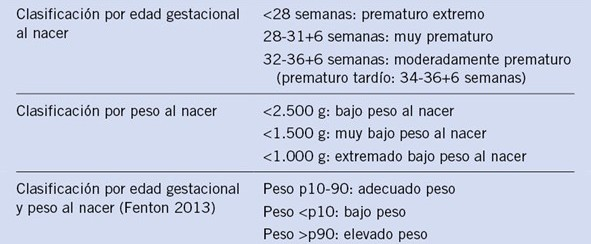
\includegraphics[width=0.75\linewidth]{img/EG.jpg}
    \caption{Clasificación de la prematuridad según la EG y el peso al nacer. Fuente: \cite{seneo2023protocolos}.}
    \label{fig:clasificación}
\end{figure}

La prematuridad representa el mayor desafío clínico actual de la Medicina Perinatal, siendo la principal causa de mortalidad infantil en menores de cinco años. La mayor parte de las complicaciones graves (morbimortalidad) se presenta en los recién nacidos “muy pretérminos”, cuya EG es inferior a 32 semanas y especialmente a los “prematuros extremos” \cite{rellan2008prematuro}.

\begin{figure}[H]
    \centering
    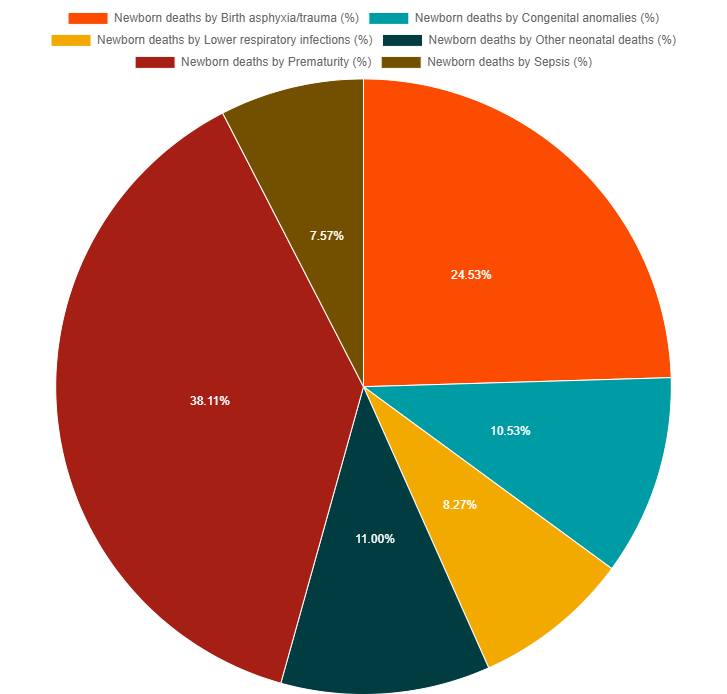
\includegraphics[width=0.7\linewidth]{img/causas.png}
    \caption{Principales causas de muerte infantil 2022 en todo el mundo 
    \\Fuente: \cite{hnn2024comprender}.}
    \label{fig:causas}
\end{figure}


Las tasas de supervivencia muestran diferencias significativas entre países: en naciones de bajos ingresos, alrededor del 50\% de los bebés nacidos a las 32 semanas o antes no sobreviven debido a la falta de atención adecuada y costo-eficaz, como el suministro de calor y el apoyo para la lactancia. En cambio, en países de altos ingresos, casi todos los bebés prematuros logran sobrevivir. Además, el uso ineficiente de la tecnología en países de ingresos medianos incrementa la discapacidad entre los recién nacidos prematuros que logran sobrevivir al período neonatal \cite{rios2017influencia}.

\subsubsection{Etiología} 

La mayor parte de los nacimientos prematuros ocurren debido a un parto prematuro espontáneo o a una amniorrexis prematura \footnote{rotura prematura de membranas}, representando más del 50\% de los casos. La presencia de infecciones clínicas o subclínicas es frecuente; de hecho, los cultivos fetales resultan positivos en el 60\% de los casos prematuros, frente al 20\% en los nacimientos a término. Entre las infecciones comunes se encuentran la vaginosis bacteriana y los niveles elevados de marcadores inflamatorios en el líquido amniótico. 

Otros factores de riesgo asociados a la prematuridad incluyen antecedentes de partos prematuros, condiciones socioeconómicas desfavorables, y el tabaquismo materno. La pobreza, el estrés materno, y el acceso limitado a la atención prenatal también son factores que incrementan el riesgo de un parto prematuro \cite{rellan2008prematuro}.

\subsubsection{Mortalidad en recién nacidos prematuros}

El riesgo de morbimortalidad está directamente relacionado con las semanas de gestación al nacer y con el peso (\ref{fig:Morbimortalidad}), pero también con el hecho de hacerlo en un lugar con el nivel asistencial adecuado \cite{COSTAS2005}.

\begin{figure}[H]
    \centering
    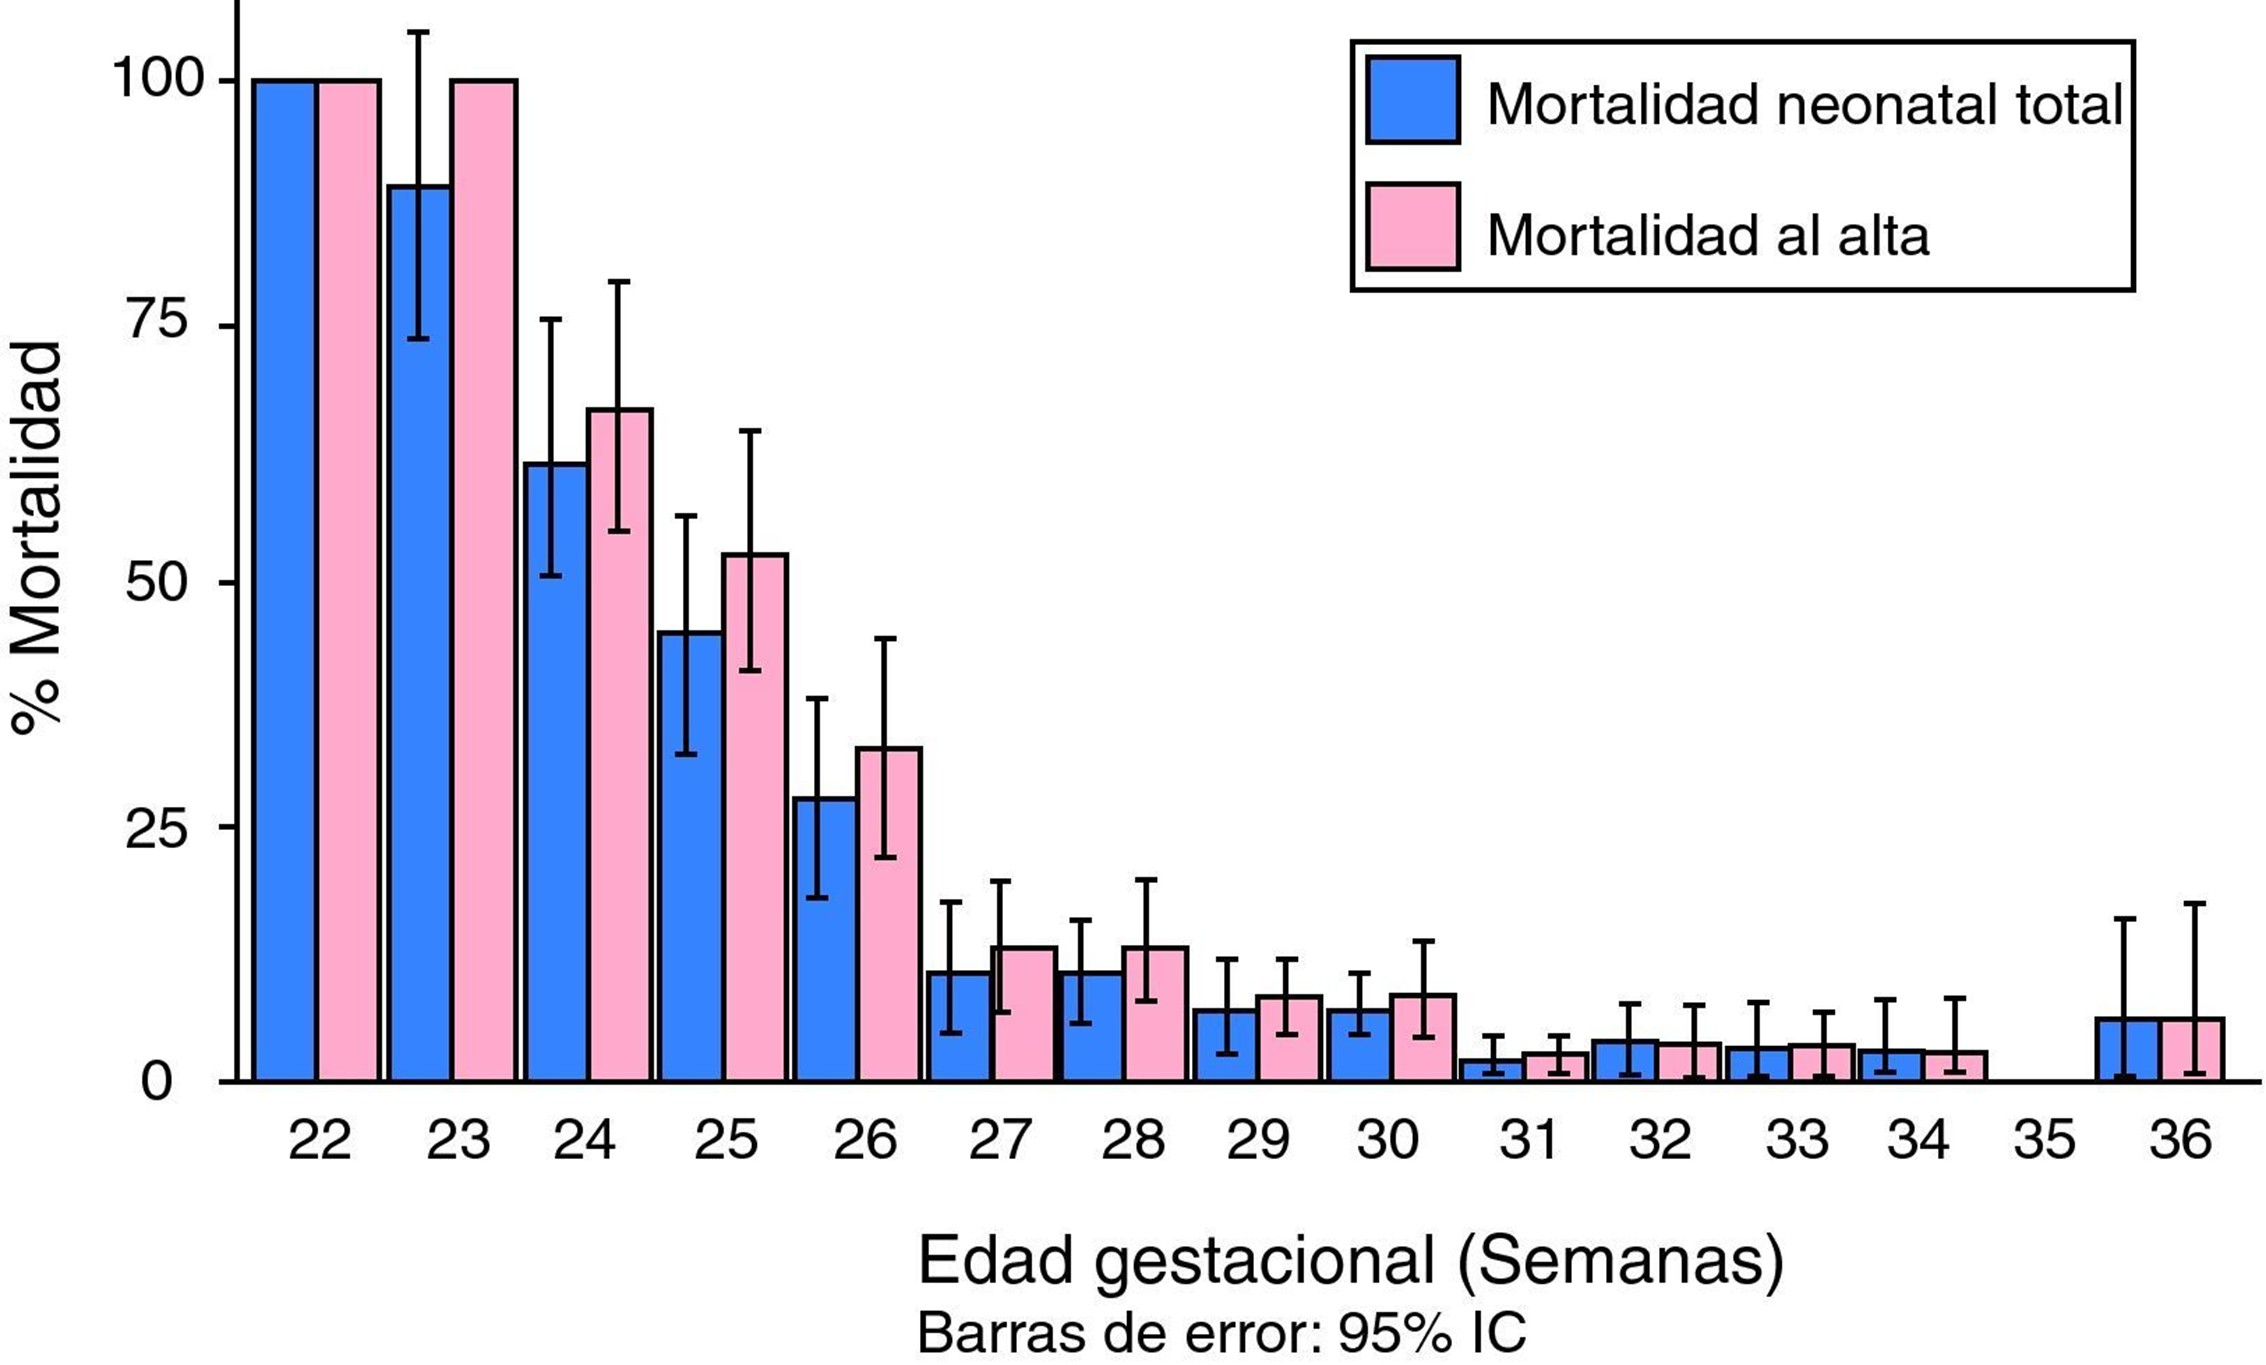
\includegraphics[width=0.7\linewidth]{img/Morbimortalidad.jpg}
    \caption{Representación de cómo se relaciona la morbimortalidad con el peso y la EG. Fuente: \cite{santesteban2012mortalidad}.}
    \label{fig:Morbimortalidad}
\end{figure}

Los recién nacidos prematuros enfrentan una serie de patologías debido a la inmadurez de sus órganos y sistemas, lo que genera una alta morbimortalidad y un motivo para que estos pacientes sean monitorizados de forma continua. A continuación, se enumeran algunas de las patologías más comunes junto con sus respectivos tratamientos:

\begin{itemize}
    \item \textbf{Patología Respiratoria:}
    Las complicaciones respiratorias son especialmente frecuentes, dado que los pulmones suelen estar poco desarrollados al momento del parto. Entre los problemas más comunes se encuentran:
    \begin{itemize}
        \item Enfermedad de Membrana Hialina (EMH): También conocida como síndrome de distrés respiratorio, esta patología está relacionada con el déficit de surfactante, una sustancia que evita el colapso de los alvéolos. El uso de CPAP (presión positiva continua en las vías respiratorias) es común para estabilizar a los bebés con esta condición
        \item Apnea del Prematuro: Los neonatos prematuros a menudo presentan episodios de apnea, donde dejan de respirar por periodos cortos de tiempo debido a la inmadurez de sus centros respiratorios en el cerebro. El monitoreo continuo de la saturación de oxígeno es importante para evitar este tipo de situaciones.
    \end{itemize}
    \item \textbf{Patología Neurológica: }El sistema nervioso central es vulnerable a la hipoxia y a las fluctuaciones hemodinámicas. Esto incrementa el riesgo de hemorragias intraventriculares (HIV) y leucomalacia periventricular\footnote{Lesión cerebral que afecta principalmente a bebés prematuros, caracterizada por la muerte o daño de la sustancia blanca alrededor de los ventrículos cerebrales.}. Se suele mantener un control preventivo de la oxigenación y la presión arterial, evitando cambios bruscos que puedan dañar el tejido cerebral.
    \item \textbf{Patología Cardiovascular: }Es frecuente que el conducto arterioso (una conexión que en la etapa fetal une la aorta con la arteria pulmonar) no se cierre después del nacimiento. Esta condición, conocida como persistencia del conducto arterioso (PCA), puede sobrecargar el sistema circulatorio y dificultar la oxigenación adecuada. Normalmente se intenta tratar con fármacos y, si no funciona, a veces hay que intervenir quirúrgicamente.
    \item \textbf{Patología Gastrointestinal:} El sistema digestivo en estos pacientes aún no está preparado para tolerar bien la nutrición, lo que incrementa el riesgo de enterocolitis necrotizante (EN), una afección grave que puede comprometer la integridad intestinal.
    \item \textbf{Inmunodeficiencia: }La incapacidad del recién nacido para contener una infección en un único órgano o sistema hace que, infecciones que en principio puedan estar controladas, sean sinónimo de una sepsis. 
\end{itemize}

Las patologías cuyos tratamientos no están mencionados no se consideran relevantes para el objetivo final de este trabajo \cite{rellan2008prematuro}.

\subsubsection{Epidemiología de la morbimortalidad}

La tasa de mortalidad infantil es uno de los indicadores más relevantes de la salud a nivel global, ya que proporciona información sobre las condiciones socioeconómicas en las que viven no solo los niños menores de 5 años, sino también el resto de la población, incluidos los adultos. Este indicador refleja, en particular, el estado de la atención perinatal, donde se observan diferencias significativas entre los países desarrollados y aquellos en vías de desarrollo.

Se relaciona con: el nivel socioeconómico, la salud materna, el acceso oportuno a los servicios de salud adecuados, la calidad en la atención y las políticas públicas en materia de salud materna y perinatal \cite{santesteban2012mortalidad}. También permite evaluar el estado de salud de las madres, las condiciones sanitarias e higiénicas, y las políticas de planificación familiar presentes en la región.

El Grupo Interinstitucional de las Naciones Unidas para la Estimación de la Mortalidad Infantil recopila y publica datos actualizados sobre la tasa de mortalidad infantil a nivel mundial, expresada en número de muertes por cada 1.000 nacidos vivos.  En la figura \ref{fig:epidemiologia} se representa la distribución de esta tasa por regiones:

\begin{figure}[H]
    \centering
    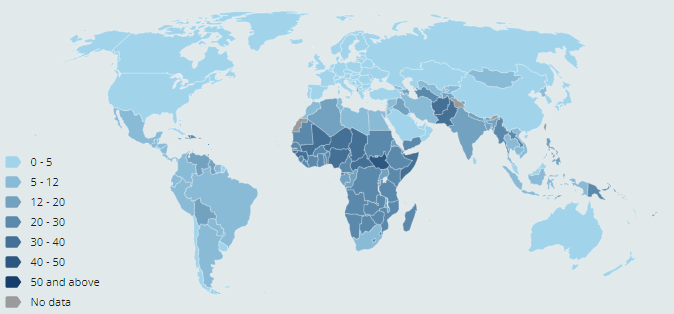
\includegraphics[width=0.9\linewidth]{img/epidemiologia.png}
    \caption{Tasa de mortalidad neonatal por cada 1.000 nacidos vivos (estimaciones globales más recientes). 
    \\ Fuente: \cite{unigme2024}.}
    \label{fig:epidemiologia}
\end{figure}

En las últimas décadas, ha habido importantes avances en la reducción de la mortalidad infantil, descendiendo un 51\% (de 37 muertes por cada 1000 nacidos vivos en 1990 a 18 en 2021) Actualmente, sobreviven más niños que nunca. Esto demuestra que es posible avanzar cuando se destinan suficientes recursos a la atención primaria de salud, lo que incluye la salud y bienestar infantiles.

Sin embargo, aún existen grandes desigualdades entre regiones y países. A nivel regional, África subsahariana y Asia meridional registran las tasas más altas de mortalidad neonatal, con 27 y 23 muertes por cada 1000 nacidos vivos, respectivamente, en 2021. Un bebé nacido en África subsahariana tiene diez veces más probabilidades de morir en su primer mes de vida que uno nacido en un país de ingresos altos, mientras que en Asia meridional ese riesgo es nueve veces mayor.


Dados todos estos datos estadísticos, es evidente que se necesita seguir invirtiendo en cuidados a los recién nacidos prematuros, sobre todo en aquellos lugares donde el acceso a los recursos se ve limitado.

\subsection{Tecnología aplicada a la prematuridad: La Incubadora neonatal}

La evidencia científica y los resultados de programas para reducir la mortalidad neonatal han permitido identificar intervenciones efectivas que, a corto y medio plazo, pueden tener un gran impacto en la supervivencia de los recién nacidos. 

Una de las soluciones más efectivas y consolidadas para abordar este problema ha sido la incubadora neonatal. Este dispositivo proporciona un entorno controlado y seguro para los recién nacidos que requieren cuidados adicionales, especialmente aquellos nacidos prematuramente o con condiciones de salud que los ponen en riesgo. 

Las incubadoras permiten recrear condiciones similares a las del vientre materno, favoreciendo que los bebés mantengan una temperatura estable y evitando que factores externos, como infecciones o cambios en la temperatura y la humedad, pongan en peligro su vida \cite{minsa2008prevencion}.

Este proyecto trabaja con una incubadora concreta,\textit{ In$^3$ator}, en cuyo diseño nos vamos a basar para explicar los tres componentes fundamentales de estos dispositivos (figura \ref{fig:partes_in3ator}):

\begin{itemize}
    \item \textbf{La cúpula o cubierta:} actúa como una barrera protectora, aislando al bebé del medio ambiente exterior. La cubierta debe permitir la visibilidad del bebé, por si hubiera problemas que las mediciones no perciben, pero que sí se pudieran apreciar a simple vista.
    \item \textbf{El chasis:} consiste en una base metálica que alberga los componentes electrónicos, como la fuente de energía, los sensores y los sistemas de soporte vital. Sobre él se coloca el porta colchón. 
    \item \textbf{El sistema de control de variables:} es responsable de monitorear y regular las condiciones internas, muy importantes para la estabilidad y recuperación del neonato:
    \begin{itemize}
        \item \textbf{Control térmico}: Los prematuros, debido a su bajo peso, piel fina y escasa grasa subcutánea, pierden calor con facilidad. Las incubadoras solucionan estas pérdidas mediante sistemas de calefacción por convección que controlan el aire que rodea al bebé. Existen dos modos de funcionamiento: uno regula la temperatura del aire de la cámara y otro, que se basa en la temperatura medida directamente en la piel del neonato.
        \item \textbf{Control de humedad}: El aire caliente circulante para el control de la termorregulación del neonato puede deshidratar al paciente, resecando su piel y sus mucosas, lo que favorece las infecciones. Para evitarlo, las incubadoras incluyen un sistema de humidificación que mantiene la humedad relativa en valores entre el 60\% y el 90\% \cite{restrepo2007incubadora}.
    \end{itemize}
\end{itemize} 

\begin{figure}[H]
    \centering
    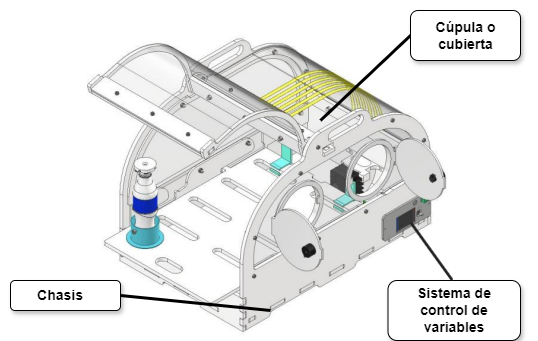
\includegraphics[width=0.65\linewidth]{img/partes_in3ator.png}
    \caption{Partes principales mencionadas de la incubadora \textit{In$^3$ator}. 
    \\ Fuente adaptada:\cite{in3es2025}. }
    \label{fig:partes_in3ator}
\end{figure}

Actualmente, la mayoría de las incubadoras modernas incluyen de forma integrada el control fisiológico del neonato a través de monitores multiparamétricos. 

De hecho, en los cuidados intensivos neonatales, la pulsioximetría se ha convertido en una herramienta importante, que aporta mucha información sobre el estado del paciente. Incorporar esta tecnología en la incubadora \textit{In$^3$ator} supone una mejora adicional, especialmente en entornos con recursos sanitarios limitados.

El siguiente bloque desarrolla los fundamentos sobre los que se basa esta tecnología y su aplicabilidad dentro del proyecto.


\section{Pulsioximetría}

La pulsioximetría es un procedimiento médico diseñado para medir la saturación de oxígeno en la sangre arterial (SaO$_2$), es decir, el porcentaje de hemoglobina que transporta oxígeno. Además, esta técnica permite cuantificar la frecuencia cardíaca y la amplitud del pulso.

\subsection{Fundamentos fisiológicos}

A continuación se describe en detalle la base fisiológica que utiliza la técnica y de dónde provienen los parámetros que mide:

\subsubsection{Sistema Cardiovascular}

El sistema cardiovascular, también conocido como sistema circulatorio, es uno de los sistemas vitales del cuerpo humano. Se encarga de transportar sangre, nutrientes, oxígeno, hormonas y de eliminar desechos metabólicos, a través de una extensa red de vasos sanguíneos y órganos especializados, siendo el corazón el protagonista de este proceso. 

El corazón, ubicado en la cavidad torácica y protegido por el pericardio, actúa como una potente bomba muscular. Su estructura se organiza en cuatro cavidades: dos aurículas y dos ventrículos. Las aurículas reciben la sangre; la aurícula derecha recoge la sangre desoxigenada proveniente del cuerpo a través de las venas cavas, mientras que la aurícula izquierda recibe la sangre oxigenada de los pulmones a través de las venas pulmonares. Posteriormente, los ventrículos se encargan de impulsar la sangre: el ventrículo derecho envía la sangre a los pulmones para que se oxigene, mientras que el ventrículo izquierdo bombea la sangre oxigenada hacia el resto del organismo a través de la aorta. Esta disposición garantiza una separación funcional entre la circulación pulmonar y la sistémica (figura \ref{fig:ciruclacion}), permitiendo que cada sistema cumpla su función de manera eficiente. 

\begin{figure}[H]
    \centering
    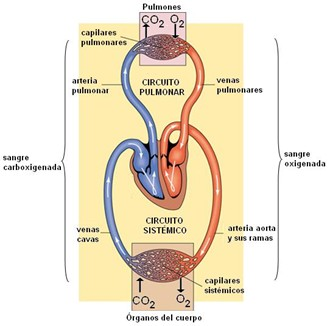
\includegraphics[width=0.55\linewidth]{img/ciruclacion.jpg}
    \caption{Representación de la circulación pulmonar y sistémica. Fuente: \cite{genomasur_cap13}.}
    \label{fig:ciruclacion}
\end{figure}

Además de su función de transporte, el sistema cardiovascular participa en la regulación de la temperatura corporal, el equilibrio de líquidos y electrolitos, y en la respuesta a las demandas metabólicas del organismo. Estos procesos se ajustan mediante la acción del sistema nervioso autónomo y diversas señales hormonales, lo que permite que el flujo sanguíneo se adapte de forma dinámica a las diferentes necesidades del cuerpo, ya sea en reposo o durante la actividad física \cite{kenhub2025}.\\



\subsubsection{Transporte del oxígeno en sangre }
El transporte de oxígeno es un proceso que garantiza el buen funcionamiento de los sistemas que componen el organismo. El oxígeno es indispensable para el metabolismo celular, ya que se utiliza en la respiración celular para generar energía en forma de adenosín trifosfato (ATP). Este proceso comienza con la inspiración de aire y culmina con la entrega de oxígeno a las células y tejidos a través del sistema circulatorio.\\ 

En la parte superior del sistema respiratorio, se encuentran la fosa nasal y la faringe, que conforman el sistema respiratorio superior. Estos órganos actúan como la primera línea de defensa, acondicionando el aire al filtrarlo, humidificándolo y calentándolo antes de que continúe su trayecto hacia el interior del aparato respiratorio. A partir de la laringe, el aire es conducido por la tráquea, la cual se ramifica en los bronquios y estos en bronquiolos, estructuras que componen el sistema respiratorio inferior. Este tramo se encarga de transportar el aire hasta los pulmones, donde se encuentran los alvéolos \cite{kenhubSistemasCuerpo2025}. \\

Cuando el aire entra en los pulmones y llega a los alvéolos pulmonares, el oxígeno se difunde a través de la membrana alveolar y se une a la hemoglobina, una proteína presente en los glóbulos rojos con gran afinidad por este gas. Cada molécula de hemoglobina puede transportar hasta cuatro moléculas de oxígeno, lo que permite una eficiente distribución a los tejidos.  \\

\begin{figure}[H]
    \centering
    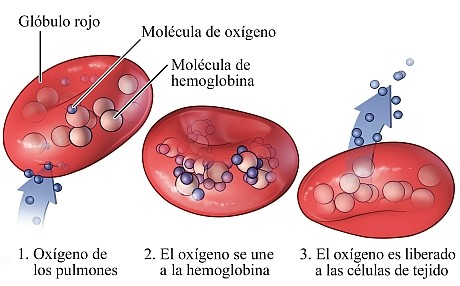
\includegraphics[width=0.6\linewidth]{img/hb.jpg}
    \caption{Transporte de oxígeno en sangre a través de la hemoglobina oxigenada. Fuente: \cite{cigna_hemoglobina}.}
    \label{fig:hb}
\end{figure}

Una vez que la sangre oxigenada llega a los tejidos a través de la circulación sistémica, los glóbulos rojos liberan el oxígeno, que difunde hacia las células. En su interior, el oxígeno es utilizado por las mitocondrias durante la fosforilación oxidativa, proceso mediante el cual se produce ATP, la principal fuente de energía celular. \\


\subsubsection{Parámetros fisiológicos relevantes en pulsioximetría}
Dado que la distribución de oxígeno depende de la eficiencia del transporte sanguíneo, es necesario medir ciertos parámetros fisiológicos para evaluar el estado hemodinámico y de oxigenación del organismo.

\newpage

\textbf{Frecuencia cardíaca}

La frecuencia cardíaca es uno de los signos vitales o indicadores más importantes para estimar la salud del cuerpo humano. Se trata del número de latidos que el corazón registra cada minuto, es decir, las veces que el corazón se contrae durante este tiempo \cite{enfermeriaCardiologia2025}.   

Varía a lo largo del día y de la noche y en respuesta a diferentes estímulos, como la actividad física, las amenazas o las emociones, por lo que su medición tiene gran variabilidad \cite{fundacionCorazon2025}.

Como norma general, la frecuencia normal en reposo de un adulto sano oscila entre 60 y 100 latidos por minuto (BPM); sin embargo, los recién nacidos tienen una frecuencia cardíaca elevada, oscilando entre 120 y 160 BPM, dado que la actividad de su organismo es muy intensa. 


\textbf{Saturación de Oxígeno (SaO$_2$)}

La hemoglobina, presente en los glóbulos rojos, se enlaza con el oxígeno en los alvéolos pulmonares para formar oxihemoglobina, que luego transporta el oxígeno a los tejidos donde se libera para ser utilizado por las células. Una vez liberado el oxígeno, la hemoglobina en su forma desoxigenada puede unirse al dióxido de carbono y llevarlo de vuelta a los pulmones para su eliminación durante la exhalación.  

La saturación de oxígeno (\ref{eq:sao2} o \ref{eq:sao2_2}) es el parámetro que se utiliza para expresar la cantidad de oxihemoglobina (HbO$_2$) respecto a la hemoglobina total (HbO$_2$ + Hb) que hay presente en nuestro organismo; es decir, describe el grado de capacidad de transporte del oxígeno en sangre \cite{gonzalez2019pulsioximetro}.

Se puede expresar como:

\begin{equation}
    SaO_2 = \frac{HbO_2}{HbO_2 + Hb} = \frac{c_{HbO_2}}{c_{HbO_2} + c_{Hb}}
    \label{eq:sao2}
\end{equation}

\begin{equation}
    SaO_2(\%) = \frac{HbO_2}{HbO_2 + Hb} \times 100\% = \frac{c_{HbO_2}}{c_{HbO_2} + c_{Hb}} \times 100\%
    \label{eq:sao2_2}
\end{equation}

\begin{center}
    Fuente: \cite{Alarco2015}.
\end{center}

En un adulto sano, los valores normales de saturación fluctúan entre el 95-100\%. Valores por debajo del 95\% (en reposo) se asocian con situaciones patológicas y del 92\% al 90\% con insuficiencia respiratoria crónica previa. En cambio, los valores normales de saturación de oxígeno en neonatos oscilan entre el 91\% y el 95\% \cite{vento2014oxigenoterapia}. 


Medir la saturación de oxígeno ayuda a evaluar la eficiencia del transporte de oxígeno y el funcionamiento pulmonar, ya que indica el grado de eficacia de un paciente en su respiración y cómo el oxígeno está siendo transportado a través del cuerpo \cite{weinmannEmergency2025}.

\subsection{Principios Físicos de la Medición Óptica }

La pulsioximetría se basa en una serie de principios físicos y ópticos que permiten estimar los parámetros fisiológicos a través de la interacción de la luz con los tejidos:


\subsubsection{Ley de Beer-Lambert}

La ley de Beer-Lambert fue descubierta independientemente (y de distintas maneras) por Pierre Bouguer en 1729, Johann Heinrich Lambert en 1760 y August Beer en 1852. Es una descripción empírica que relaciona la absorción de la luz con las propiedades del material que atraviesa \cite{Gilsanz2023}.

Describe cómo la intensidad de la luz que pasa a través de un medio absorbente disminuye en función de la concentración de la sustancia absorbente, la longitud del trayecto de la luz a través del medio, y el coeficiente de absorción específico de esa sustancia. Se puede expresar de dos maneras:

En su forma logarítmica (\ref{eq:ley_beer}), como absorbancia:

\begin{equation}
    A = \varepsilon \cdot b \cdot C 
    \label{eq:ley_beer}
\end{equation}


\begin{itemize}
    \item A es la absorbancia.
    \item $\varepsilon$ es el coeficiente de absorción (o extinción) del cromóforo\footnote{Un cromóforo es una parte de una molécula que absorbe luz visible o UV, lo que le da a la molécula un color.}
    \item b es la longitud del camino recorrido por la luz. 
    \item c es la concentración de las especies absorbentes. 
\end{itemize}

\newpage

O en forma exponencial (\ref{eq:ley_beer2}), como transmisión de luz:

\begin{equation}
    I = I_0 a^{-\mu \dot{d}} 
    \label{eq:ley_beer2}
\end{equation}

\begin{itemize}
    \item I= Intensidad de luz después de atravesar el medio.
    \item I$_0$ = Intensidad de luz inicial.
    \item $\mu$ = Coeficiente de atenuación. 
    \item d = Longitud del camino óptico.
\end{itemize}


\begin{figure}[H]
    \centering
    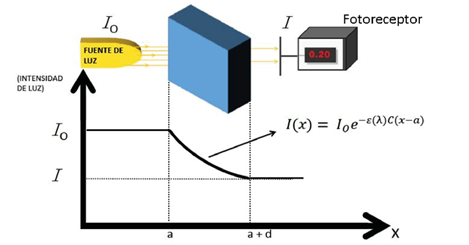
\includegraphics[width=0.75\linewidth]{img/beerlambert.png}
    \caption{Transmisión de luz a través de un medio absorbente según la Ley de Beer-Lambert. 
    \\ Fuente: \cite{Cordido2023}.}
    \label{fig:beerlambert}
\end{figure}

Ambas expresiones muestran que cuanto más absorbente es el medio, menos luz llegará al sensor, lo que permite estimar la concentración del compuesto de interés. 

En el caso de la pulsioximetría, el medio absorbente es el tejido del paciente, y el compuesto de interés es la hemoglobina, en sus dos formas: oxigenada (HbO$_2$) y reducida (Hb). Los tejidos biológicos y la sangre absorben luz en diferentes proporciones, y la hemoglobina es el principal cromóforo en la sangre que absorbe en el rango visible e infrarrojo cercano.

\begin{itemize}
    \item HbO$_2$ absorbe más luz en la región infrarroja (910–940 nm).
    \item Hb absorbe más luz en la región roja (640–660 nm).
\end{itemize}

\begin{figure}[H]
    \centering
    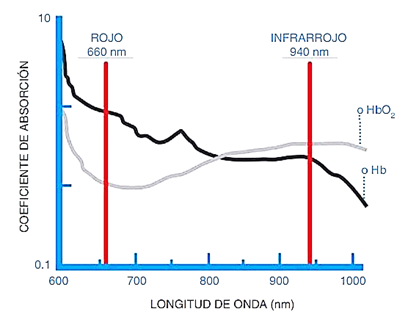
\includegraphics[width=0.6\linewidth]{img/absorbancia.png}
    \caption{Absorción de la hemoglobina y la oxihemoglobina en dos longitudes de onda. Fuente: \cite{DeLaPena2017}.}
    \label{fig:absorbancia}
\end{figure}

Por eso, los pulsioxímetros utilizan dos longitudes de onda distintas: una roja y otra infrarroja. Al medir cuánta luz de cada tipo atraviesa el tejido, el dispositivo puede calcular la proporción entre ambas formas de hemoglobina. 


\subsubsection{Señal de Fotopletismografía}

La fotopletismografía (PPG) es una técnica óptica utilizada para medir los cambios en el volumen sanguíneo mediante la detección de variaciones en la absorción de luz. Esta técnica es la base de funcionamiento de un pulsioxímetro. 

El principio de la PPG se basa en la emisión de luz a través de un transductor, que atraviesa los tejidos del paciente y es captada por un fotodetector. La cantidad de luz absorbida varía en función de los cambios en el volumen sanguíneo en los vasos, de acuerdo con la ley de Beer-Lambert, lo que permite registrar una señal que puede ser procesada para extraer información fisiológica relevante.

La señal obtenida mediante PPG presenta dos componentes principales: 

\begin{itemize}
    \item \textbf{Componente pulsátil o corriente alterna (AC): }Representa las variaciones periódicas asociadas con el ciclo cardíaco, directamente vinculadas con el volumen de sangre arterial impulsado por el corazón. Esta componente permite calcular la frecuencia cardíaca. 
    \item \textbf{Componente no pulsátil o corriente continua (DC): }Se debe a la absorción de luz por los tejidos circundantes, como la piel, la grasa subcutánea, los músculos y los huesos, así como la sangre venosa y capilar. Esta componente permite analizar la diferencia de absorción entre los dos tipos de luz utilizados en la medición (roja e infrarroja)\cite{DeLaPena2017}.
\end{itemize}

\begin{figure}[H]
    \centering
    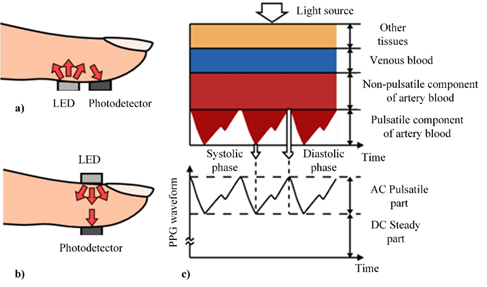
\includegraphics[width=0.7\linewidth]{img/PPG.png}
    \caption{Partes de la señal PPG. Fuente:\cite{Dzedzickis2020}.}
    \label{fig:PPG}
\end{figure}

Durante la sístole, el corazón bombea sangre hacia las arterias, aumentando el volumen sanguíneo en los capilares del área donde está colocado el sensor PPG. Como hay más sangre arterial, la absorción de luz infrarroja y roja aumenta, lo que reduce la intensidad de la luz detectada por el fotodetector. En la señal PPG, esto se observa como un pico (máxima amplitud).

Durante la diástole (relajación del corazón), el volumen sanguíneo en los capilares disminuye porque la sangre fluye de regreso al corazón. Al haber menos sangre arterial, la absorción de luz disminuye y más luz llega al fotodetector. En la señal PPG, esto se observa como un valle (mínima amplitud).


Esta señal es la base de la que partimos en el proyecto, y hablaremos sobre su tratamiento en la sección \ref{cap: Metodología}.

\subsection{Aplicación: El pulsioxímetro}

Todo lo expuesto hasta ahora se materializa en un dispositivo compacto y portátil: el pulsioxímetro. Este instrumento permite monitorizar en tiempo real la saturación de oxígeno y la frecuencia cardíaca del paciente, de forma continua y no invasiva. 

Está compuesto por un sensor con un diodo emisor de luz roja e infrarroja (LED) y un fotodiodo detector, los cuales están conectados al oxímetro (monitor) mediante un cable. El sensor mide cuánta luz de cada longitud de onda llega al fotodetector y, a partir de ahí, se calcula un cociente que se relaciona con la proporción de hemoglobina oxigenada.

\begin{figure}[H]
    \centering
    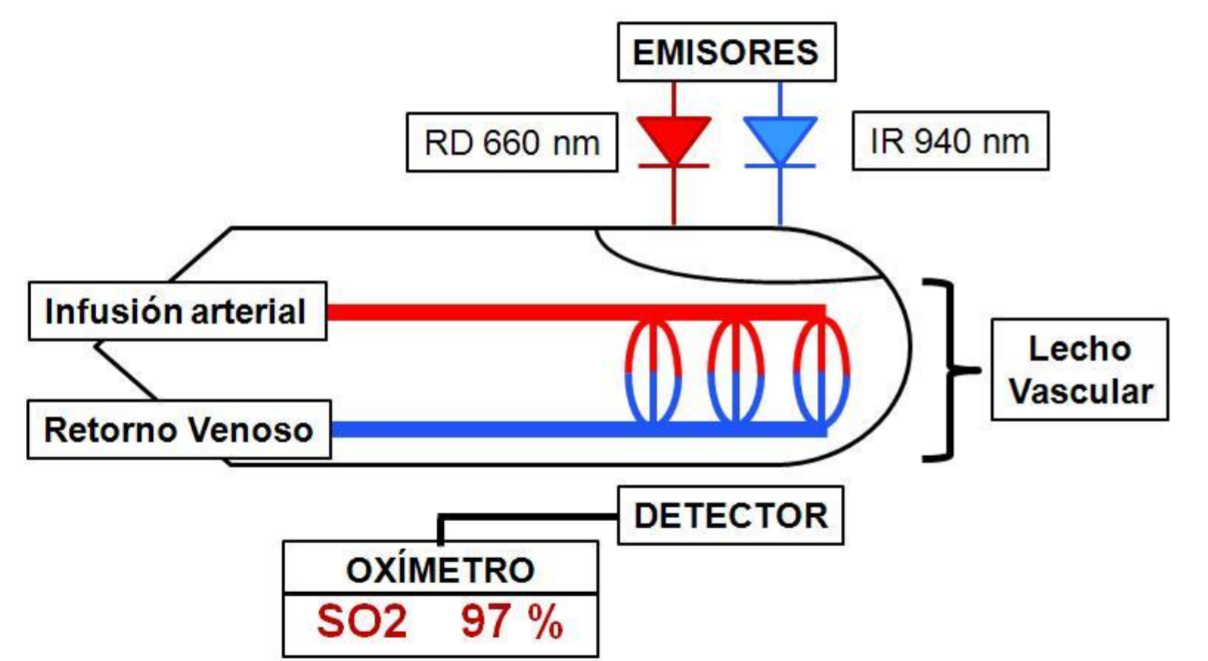
\includegraphics[width=0.6\linewidth]{img/pulsioximetrofuncionamiento.png}
    \caption{Esquema de funcionamiento y partes de un pulsioxímetro.
    \\ Fuente: \cite{medicinajoven_pulsioximetro}. }
    \label{fig:pulsioximetro}
\end{figure}

A medida que la luz pasa a través de la sangre pulsátil, la hemoglobina absorbe una de las longitudes de onda y deja pasar la otra, dependiendo de su estado de oxigenación. Cuando la hemoglobina está unida al oxígeno, refleja la luz roja y absorbe la infrarroja, lo que le confiere un color rojo brillante. En ausencia de oxígeno, la hemoglobina absorbe la luz roja y refleja la infrarroja, adquiriendo un tono rojo oscuro \cite{imfesPulsioximetro2025}.\\

El sensor detecta estas variaciones debidas a los cambios en el volumen arterial y, mediante algoritmos de calibración basados en datos experimentales, el dispositivo determina la proporción relativa de hemoglobina oxigenada en sangre y calcula automáticamente los valores de SpO$_2$\footnote{A partir de este punto se empleará el término \textbf{SpO$_2$}, que hace referencia a la saturación periférica de oxígeno estimada mediante pulsioximetría, en lugar de \textbf{SaO$_2$}, que corresponde a la saturación arterial medida de forma invasiva mediante análisis de gases en sangre. Aunque no son equivalentes, la SpO$_2$ se utiliza como una aproximación clínica habitual de la SaO$_2$.}
 y frecuencia cardíaca.

La señal PPG del pulsioxímetro se puede obtener a través de dos configuraciones del sensor:

\begin{itemize}
    \item \textbf{Reflectiva:} Ambos componentes (LED y fotodetector) están en el mismo lado.
    \item \textbf{Transmisiva :} Se usa cuando el LED y el fotodetector están en lados opuestos del tejido (ej., en un lóbulo de la oreja o el dedo).
\end{itemize}

En la parte práctica, utilizamos un sensor de tipo transmisivo, en el que la luz atraviesa el tejido antes de ser captada por el fotodetector.


\subsubsection{Factores que pueden afectar a la medición }

En muchos casos, las mediciones de los pulsioxímetros en atención médica pueden verse afectadas por varias circunstancias:

\begin{itemize}
\item \textbf{Movimiento}

El movimiento es una de las principales fuentes de error en la medición de SpO$_2$, especialmente en recién nacidos. La oximetría de pulso convencional asume que solo la sangre arterial presenta un componente pulsátil, pero el movimiento también genera variaciones ópticas y desplazamiento de sangre venosa. Esto puede hacer que el pulsioxímetro interprete erróneamente la señal venosa como arterial, reduciendo la precisión de la medición y generando valores falsamente bajos.

\item \textbf{Baja perfusión}

Cuando la perfusión disminuye (por hipotermia o bajo gasto cardíaco), la señal pulsátil se reduce y puede acercarse al nivel de ruido del pulsioxímetro. En casos extremos, la señal fisiológica queda enmascarada, afectando la precisión de la medición. 

\item \textbf{Interferencias externas}

\begin{itemize}
    \item Pigmentación de la piel: La piel oscura y ciertos esmaltes absorben luz a 660 nm y 940 nm, afectando la medición de SpO$_2$ en niveles bajos. 
    \item Interferencia electromagnética: Equipos como tomógrafos, aparatos quirúrgicos eléctricos o teléfonos móviles pueden alterar la lectura y causar sobrecalentamiento del sensor. 
    \item Luz ambiental: La exposición a luces intensas (quirófano, fototerapia) puede interferir con la lectura.
\end{itemize}


\item \textbf{Variantes de hemoglobina}

\begin{itemize}
    \item Carboxihemoglobina (COHb): Puede sobreestimar la SpO$_2$ en pacientes expuestos al monóxido de carbono, como fumadores o intoxicados. 
    \item Metahemoglobina: En casos de intoxicación por fármacos o anestésicos, altera la absorción de luz y genera mediciones imprecisas. 
\end{itemize}

\item \textbf{Oximetría de pulso en altura}

A nivel del mar, la SpO$_2$ normal es 97-99\% (límite inferior: 94\%). A mayores altitudes (>2500 msnm), la presión de oxígeno disminuye, adaptando los niveles de SpO$_2$. En niños sanos que residen en altura, valores entre 85-87\% pueden considerarse normales. \cite{oximetria_pulso2012}

\end{itemize}

\section{Procesamiento Digital de Señales Biomédicas}

Después de haber explicado en qué consiste la pulsioximetría, el siguiente paso es entender cómo se trabaja con las señales que genera el sensor. Estas señales, aunque contienen información relevante, no siempre son claras ni fáciles de interpretar.

El organismo se comunica consigo mismo a través de señales de diversa naturaleza, que en el cuerpo humano se reducen a la energía eléctrica, química, mecánica y térmica. Estas señales biomédicas contienen información valiosa sobre los procesos fisiológicos, aunque dicha información no siempre es perceptible. En muchos casos, la información útil se encuentra oculta en la estructura de la señal, requiriendo ser decodificada o extraída mediante técnicas adecuadas de análisis \cite{carrion2011procesado}.


\begin{table}[H]
\centering
\begin{tabular}{|l|p{5cm}|p{6cm}|}
\hline
\textbf{Energía} & \textbf{Variables} & \textbf{Mediciones} \\
\hline
Química   & Concentración química & Concentraciones en sangre, O$_2$, CO$_2$, pH, hormonas, etc. \\ \hline
Mecánica  & Posición, torque, presión & Contracción muscular, presión cardiovascular, sonidos cardíacos, etc. \\\hline
Eléctrica & Voltaje y corriente de flujo iónico & EEG, ECG, EMG, PPG \\\hline
Térmica   & Temperatura & Termografía clínica \\
\hline
\end{tabular}
\caption{Tipos de energía, variables biológicas asociadas y ejemplos de mediciones biomédicas. Fuente: \cite{dePedroCarracedo2020}.}
\label{tabla:energia}
\end{table}


Las señales biomédicas reflejan propiedades intrínsecas de los sistemas biológicos de los que provienen, y su estudio permite identificar tanto estados normales como patológicos. En algunas situaciones, una simple inspección visual de la señal puede ser suficiente para interpretar su contenido; sin embargo, la complejidad de la mayoría de las señales fisiológicas hace necesario aplicar técnicas de procesamiento digital, que permitan extraer de forma fiable la información clínica relevante.

\subsection{Adquisición de señales biomédicas}

El procesamiento de señales biomédicas comienza con su correcta adquisición. Esta consiste en transformar una señal analógica, continua en el tiempo, en una representación digital adecuada para el tratamiento numérico. Este proceso implica el desarrollo de varias etapas:

\begin{itemize}
    \item \textbf{Captura de la señal: }mediante sensores que convierten la magnitud biológica en una señal eléctrica proporcional, por ejemplo, la absorción de luz en PPG.
    \item \textbf{Acondicionamiento}: puede incluir amplificación, filtrado analógico inicial y adaptación de la señal al rango dinámico del conversor analógico-digital (ADC).
    \item \textbf{Conversión analógico-digital (ADC):} que consiste en la discretización temporal mediante muestreo periódico y la discretización en amplitud mediante cuantificación.
\end{itemize}

Para conservar la información contenida en la señal original, el teorema de Nyquist establece que la frecuencia de muestreo debe ser, al menos, el doble de la máxima frecuencia presente en la señal. En señales de interés fisiológico, como las captadas mediante PPG, la frecuencia de muestreo suele situarse entre 50 y 200 Hz, dependiendo de la aplicación concreta.

En el caso de este proyecto, la fase de adquisición de la señal ha supuesto una gran parte del desarrollo, que se explicará en la sección \ref{cap: Metodología}.

\subsection{Filtrado digital de señales}

Es habitual que las señales, una vez adquiridas, contengan no solo la información fisiológica de interés, sino también componentes de ruido e interferencias no deseadas. El objetivo del filtrado digital es eliminar o atenuar estas perturbaciones sin distorsionar el contenido útil de la señal. Para ello, es necesario que las características del filtro se ajusten al espectro de interés. En aplicaciones biomédicas, este espectro puede variar en función del tipo de señal, del estado fisiológico del paciente y de la calidad de adquisición, lo que justifica la necesidad de adaptar los parámetros del filtro a cada caso particular \cite{studysmarter_filtro_biosenales}.

Según las necesidades del análisis, pueden emplearse distintos tipos de filtros:

\subsubsection{Según la función que realizan}

\textbf{Filtros paso bajo}

Permiten el paso de señales por debajo de una frecuencia de corte y atenúan señales por encima de la frecuencia de corte. Es decir, eliminan las componentes de alta frecuencia, como el ruido eléctrico o artefactos \cite{mathworks_lowpass_filter}.

\textbf{Filtros paso alto}

Los filtros paso alto atenúan las señales situadas por debajo de una frecuencia de corte y permiten el paso de señales situadas por encima de la frecuencia de corte. Es decir, eliminan componentes de muy baja frecuencia, como el desplazamiento de la línea base \cite{mathworks_highpass_filter}.

\textbf{Filtros paso banda}

Permiten seleccionar el rango de frecuencias donde se encuentra la información de interés, atenuando o bloqueando las frecuencias fuera de ese rango \cite{rubia2021diseno}.

\textbf{Filtros IIR (Infinite Impulse Response) }

Los filtros IIR (Respuesta Infinita al Impulso) son filtros digitales cuya respuesta al impulso teóricamente se extiende indefinidamente, ya que utilizan tanto valores pasados de la señal de entrada como de la salida filtrada \cite{gonzalez2014filtrado}, esto les permite lograr ciertos efectos de filtrado usando menos cálculos que otros filtros.

\textbf{FIR (Finite Impulse Response)}

Los filtros FIR (Respuesta Finita al Impulso) son filtros digitales cuya respuesta al impulso tiene una duración limitada en el tiempo, ya que dependen exclusivamente de valores actuales y pasados de la señal de entrada. Son estables y pueden diseñarse para tener una respuesta de fase lineal \cite{gonzalez2014filtrado}.

En la figura \ref{fig:filtros} se puede observar cómo modifica cada filtro a la señal.

\begin{figure}[H]
    \centering
    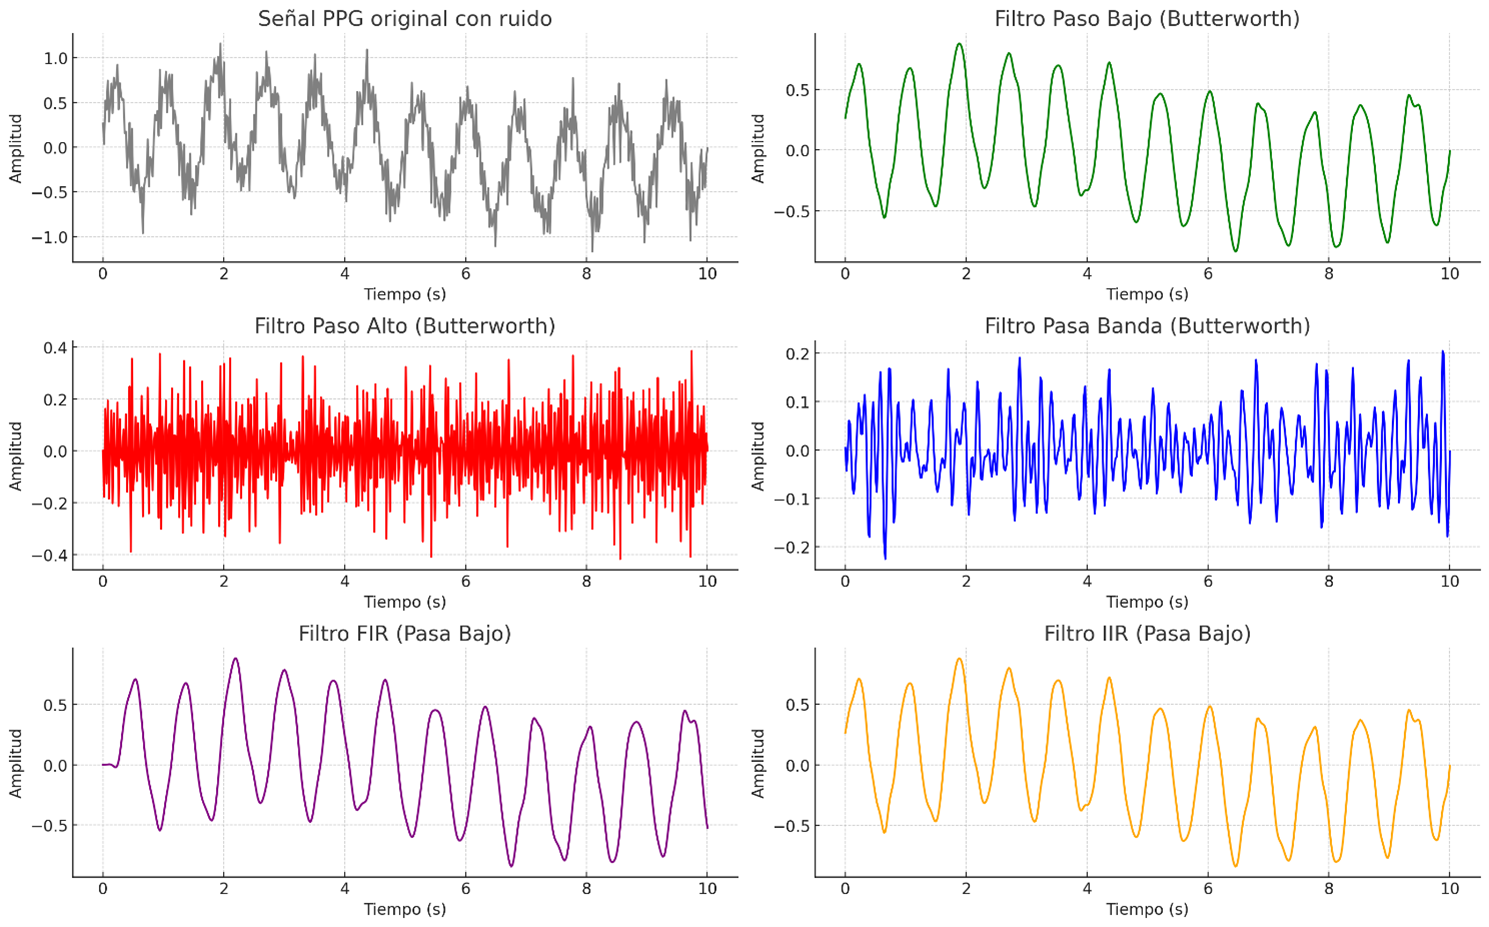
\includegraphics[width=0.92\linewidth]{img/filtros.png}
    \caption{Comparación de los tipos de filtrado mencionados a partir de una señal PPG. \textit{Elaboración propia}.}
    \label{fig:filtros}
\end{figure}

\subsubsection{Según el diseño o implementación}

\textbf{Moving Average o filtro de media móvil}

Se utiliza para suavizar las señales adquiridas. Consiste en reemplazar cada muestra de la señal por el promedio de un número fijo de muestras adyacentes. Se trata de un método simple y computacionalmente eficiente para suavizar variaciones rápidas y aleatorias en la señal. Sin embargo, puede distorsionar transiciones rápidas o picos pronunciados \cite{mathworks_lowpass_filter}.

\textbf{Filtro de Savitzky-Golay}

Este método suaviza la señal mediante un ajuste polinomial local de las muestras. A diferencia de la media móvil, el filtro de Savitzky-Golay conserva mejor la forma y amplitud de las características locales de la señal, como picos o valles, haciendo que sea especialmente útil en señales donde es importante preservar la morfología.

\textbf{Filtro Butterworth}

Los filtros de Butterworth se caracterizan por una respuesta en frecuencia plana en la banda pasante, lo que significa que no introduce oscilaciones ni altera la forma original de la señal. Además, su transición hacia la zona donde se atenúan las frecuencias no deseadas (banda de corte) es suave y progresiva, lo que ayuda a reducir el ruido sin introducir artefactos bruscos. Es una buena opción cuando se quiere mantener la señal lo más parecida posible a la original, pero más limpia.

\begin{figure}[H]
    \centering
    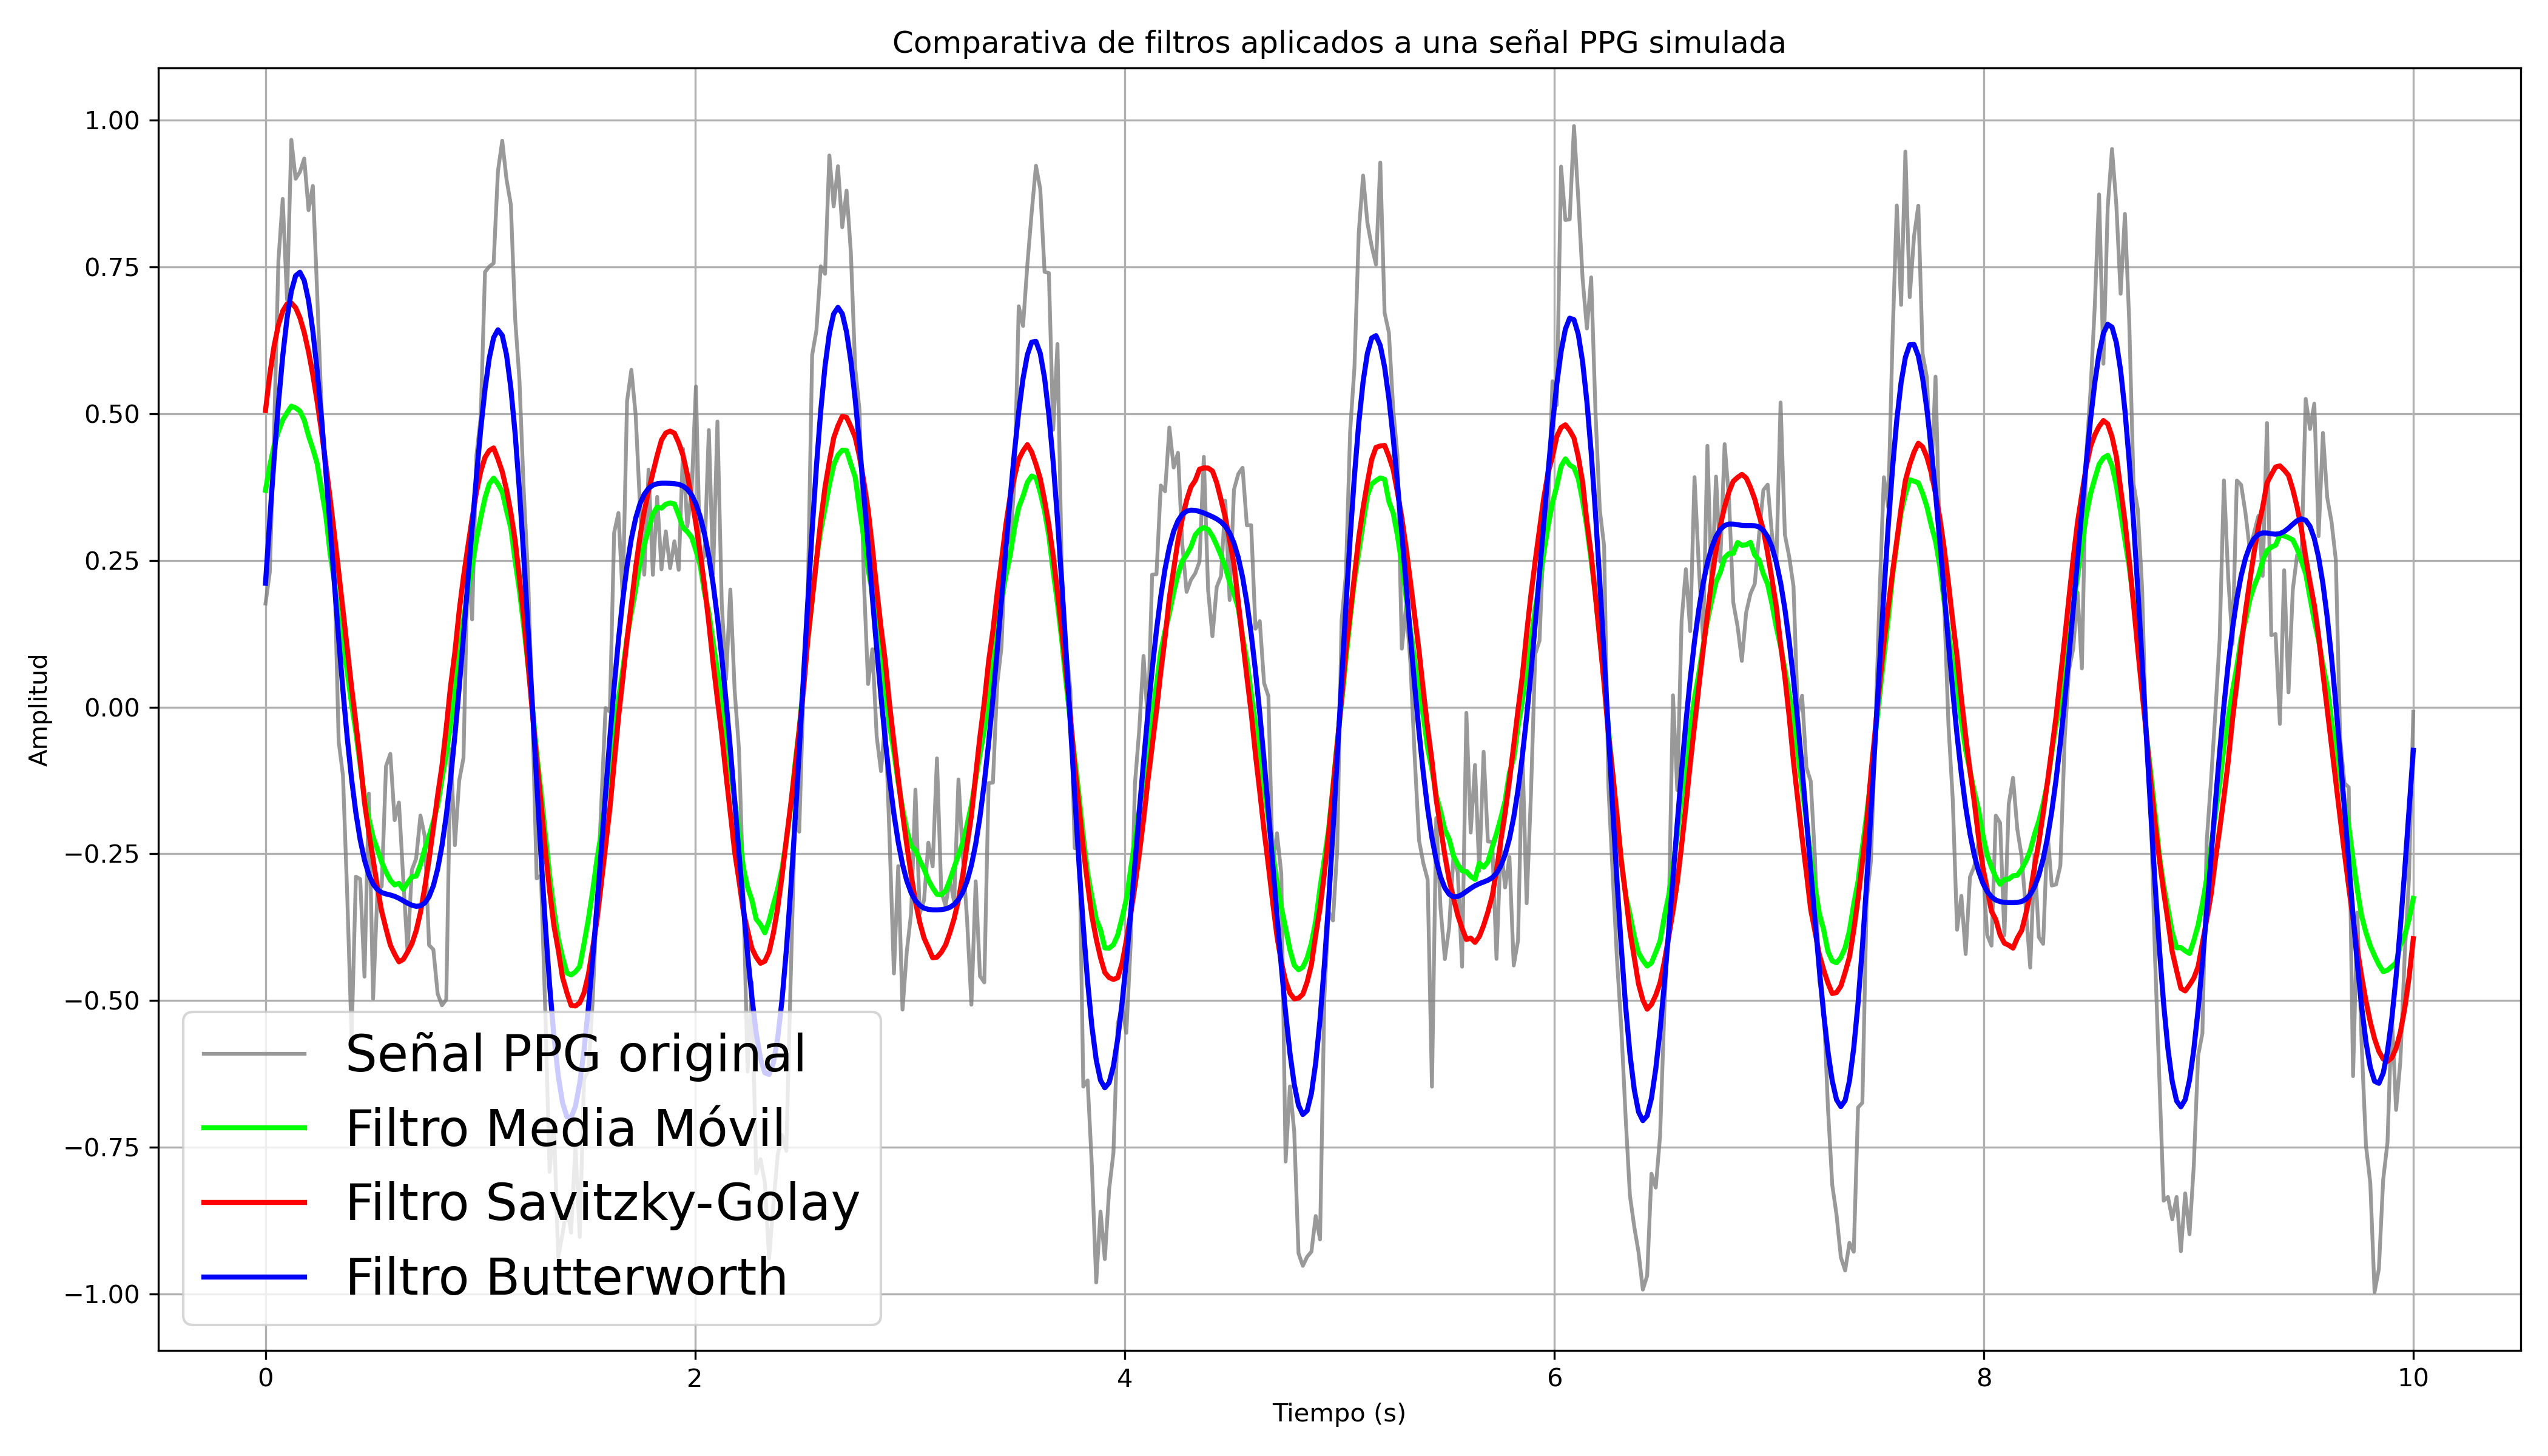
\includegraphics[width=0.85\linewidth]{img/filtrados.png}
    \caption{Comparación de los tipos de filtros según el diseño o implementación. \textit{Elaboración propia}.}
    \label{fig:filtrados}
\end{figure}

Solo se han descrito aquellos filtros que han sido implementados en este trabajo, omitiendo otros tipos cuya aplicación no ha sido necesaria para los objetivos planteados.

\subsection{Modelos y Algoritmos para la Conversión de Señales en Parámetros Clínicos}

Para que un pulsioxímetro proporcione información útil, es necesario transformar las señales ópticas captadas, en parámetros fisiológicos interpretables por un ser humano. Esta conversión se basa en modelos matemáticos y algoritmos de procesamiento de señal que permiten extraer información fiable. A continuación, se describen los fundamentos y métodos empleados para el cálculo de ambos parámetros.

\subsubsection{Cálculo de la Frecuencia Cardíaca:}

En los pulsioxímetros comerciales, la frecuencia cardíaca se estima a partir de la señal PPG, que refleja las variaciones en el volumen de sangre generadas por cada latido del corazón. Estas oscilaciones, visibles como picos en la señal, permiten identificar el momento en que ocurre cada pulso arterial.

\begin{figure}[H]
    \centering
    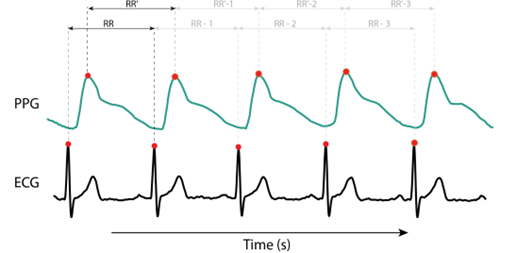
\includegraphics[width=0.75\linewidth]{img/ECGvsPPG.png}
    \caption{Comparación entre señales PPG y ECG para la medición del intervalo RR. 
    \\ Fuente: \cite{vandenberk2017fibricheck}.}
    \label{fig:ECGvsPPG}
\end{figure}

El primer paso del algoritmo suele ser aplicar un filtro para aislar el rango de frecuencias correspondiente a la actividad cardíaca, eliminando así componentes no deseadas como el ruido de alta frecuencia o las variaciones lentas del entorno \cite{liu2021wearable}.

Posteriormente, se realiza una detección de picos, normalmente sobre la componente AC de la señal infrarroja. Cada pico representa un latido cardíaco. 

A partir del intervalo temporal entre picos sucesivos (intervalos RR), se calcula la frecuencia cardíaca mediante la ecuación \ref{eq: HR}:

\begin{equation}
\text{HR (BPM)} = \frac{60}{\text{intervalo entre picos (s)}}
\label{eq: HR}
\end{equation}



Para evitar oscilaciones en la lectura, algunos dispositivos promedian el intervalo entre varios picos consecutivos. La estabilidad del cálculo depende de la calidad de la señal y del rendimiento del algoritmo de detección, que debe ser robusto frente a artefactos de movimiento o presión inadecuada del sensor.

\subsubsection{Cálculo de la Saturación de Oxígeno (SpO\textsubscript{2})}

Tal y como se ha explicado con anterioridad, la estimación de la saturación de oxígeno en sangre mediante pulsioximetría se basa en la Ley de Beer-Lambert, con la que se logra definir que la intensidad de la luz disminuye con la longitud de la trayectoria, siendo conocedores de que la señal de la luz transmitida a través del dedo está formada por una componente de corriente continua (DC) y una de corriente alterna (AC) \cite{liu2021wearable}. 

A partir de estas componentes, se calcula el \textbf{Ratio R} (\ref{eq:ratio}) característico:

\begin{equation}
    R = \frac{\frac{\mathrm{AC}_{\text{red}}}{\mathrm{DC}_{\text{red}}}}{\frac{\mathrm{AC}_{\text{IR}}}{\mathrm{DC}_{\text{IR}}}}
    \label{eq:ratio}
\end{equation}

El valor de \( R \) se relaciona experimentalmente con el porcentaje de saturación de oxígeno mediante una curva de calibración (figura \ref{fig:ratio}), obtenida mediante estudios en voluntarios sanos. Dado que resulta peligroso inducir saturaciones muy bajas (por debajo del 75\%), los pulsioxímetros extrapolan la calibración en ese rango mediante modelos matemáticos.

\begin{figure}[H]
    \centering
    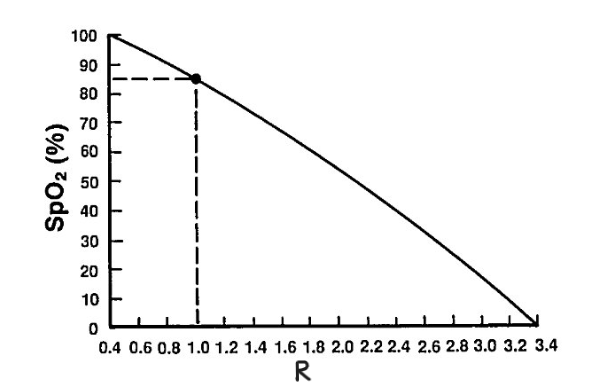
\includegraphics[width=0.55\linewidth]{img/ratio.png}
    \caption{Explicación gráfica del cálculo de la SpO$_2$ a partir de R. Fuente adaptada: \cite{deshmane2009false}.}
    \label{fig:ratio}
\end{figure}

La relación empírica adoptada por muchos dispositivos comerciales puede aproximarse mediante una ecuación lineal (\ref{eq: spo2_3}) del tipo:

\begin{equation}
    \text{SpO}_2 (\%) = A - (B \times R)
    \label{eq: spo2_3}
\end{equation}

donde \( A \) y \( B \) son constantes de calibración específicas de cada dispositivo. Por ejemplo, algunas implementaciones proponen valores como \( A = 110 \) y \( B = 25 \).

Además, para mejorar la estimación de SpO\textsubscript{2} en condiciones de baja perfusión o presencia de artefactos de movimiento, se utilizan técnicas de procesamiento digital adicionales como la \textit{Transformada Rápida de Fourier (FFT)} \cite{jimenez2019pulsioximetro}.


\section{Estado del arte y trabajos relacionados}

Se presenta a continuación una recopilación de desarrollos recientes vinculados a esta tecnología, seleccionados por su interés particular para este proyecto.

\subsection{Dispositivos comerciales y soluciones de bajo coste}

Los pulsioxímetros comerciales ofrecen alta precisión, pero su elevado coste limita su integración o adquisición en entornos con recursos limitados. Como alternativa, han surgido múltiples proyectos open-source y de bajo coste basados en sensores como el MAX30102, integrables en plataformas como Arduino \cite{llamas_pulsimetro_max30102}. 

Iniciativas como \textbf{OpenOximetry.org} \cite{openoximetry2025} proponen estándares abiertos para mejorar la precisión y validación de pulsioxímetros en contextos desfavorecidos.

\begin{figure}[H]
    \centering
    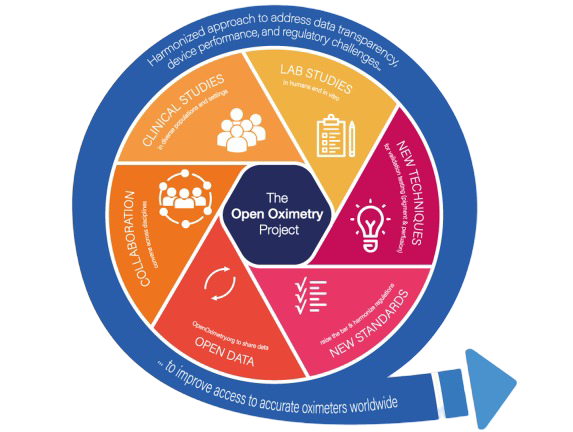
\includegraphics[width=0.6\linewidth]{img/openoximetry.png}
    \caption{Esquema del enfoque y objetivo del Open Oximetry Project. Fuente: \cite{elmankabadi2023openoximetry}.}
    \label{fig:openoximetry}
\end{figure}

\subsection{Aplicaciones en salud global y neonatología}

Durante la pandemia de COVID-19, la pulsioximetría se popularizó para el monitoreo domiciliario. En neonatología, se propone su uso para detectar afecciones frecuentes como la hipoxia o las cardiopatías congénitas. La Global Oximetry Initiative \cite{thoms2007global}, por ejemplo, es una iniciativa lanzada en el año 2007 en Uganda, India, Filipinas y Vietnam, cuyo objetivo principal es promover el uso de la oximetría y reducir sus costos en países de bajos ingresos, así como la creación de nuevas políticas, influir en su diseño y establecer nuevos estándares globales para una monitorización más segura.


\subsection{Proyectos relacionados}

Se han desarrollado numerosos prototipos de la solución tecnológica propuesta. Se mencionan brevemente los que se han considerado más relevantes: 

\begin{itemize}
    \item \textbf{Diseño y simulación de un pulsioxímetro a bajo costo}: Este proyecto de tesis propone un pulsioxímetro económico utilizando un Arduino Uno, con el objetivo de disminuir su costo en un 15\% y fomentar su fabricación local en Honduras para áreas de enfermería de CEUTEC \cite{chacon2021pulsioximetro}.
    \item \textbf{Diseño e implementación de un pulsioxímetro reflexivo y estudio de su funcionamiento en diferentes zonas del cuerpo :} Este trabajo de fin de grado se centra en el diseño de un prototipo de pulsioxímetro reflexivo utilizando el sensor MAX30102 y un microprocesador, evaluando su precisión y viabilidad para aplicaciones médicas \cite{gonzalez2019pulsioximetro}.
    \item \textbf{Pulsioxímetro con registro de datos en IoT y generación de alertas}: Este TFG propone un pulsioxímetro económico con comunicación Wi-Fi para registrar datos de frecuencia cardíaca y saturación de oxígeno en la nube mediante ThingSpeak\footnote{ThingSpeak es una plataforma de análisis de IoT que permite agregar, visualizar y analizar flujos de datos en vivo en la nube}, permitiendo generar alertas automáticas. Utiliza el sensor MAX30100 y un ESP8266 como microcontrolador \cite{sein2019pulsioximetro}.
    \item \textbf{Diseño e implementación de un pulsioxímetro orientado a deportistas de apnea}: Este proyecto desarrolla un prototipo básico de pulsioxímetro con fines deportivos, con especial atención a las condiciones de presión y temperatura extremas. Utiliza Arduino y sensores ópticos específicos, y propone mejoras de diseño para su aplicación subacuática \cite{borbones2021pulsioximetro}.
    \item \textbf{Medida del nivel de saturación de oxígeno en sangre: desarrollo de un pulsioxímetro de bajo coste y comparativa con otros sistemas existentes}: Este trabajo desarrolla un pulsioxímetro de bajo coste basado en la Ley de Beer-Lambert, usando sensores ópticos para estimar SpO$_2$ de forma no invasiva \cite{Alarco2015}.
    \item \textbf{Diseño de un pulsioxímetro de bajo coste y salida bluetooth}: Presenta el diseño e implementación de un pulsioxímetro económico que transmite datos de SpO$_2$ y pulso vía Bluetooth, orientado a su uso en telemedicina \cite{jimenez2019pulsioximetro}.
\end{itemize}


\subsection{Algoritmos de estimación de la frecuencia cardíaca}

También se ha investigado acerca de los diferentes enfoques que se han propuesto para la estimación de la frecuencia cardíaca a partir de señales PPG:

\begin{itemize}
  \item \textbf{Detección de picos en el dominio temporal:} como se ha mencionado, se trata del método más clásico y utilizado. Fue analizado por Elgendi \cite{elgendi2012analysis} y optimizado por Vourvoulakis et al. \cite{9493400} mediante un umbral adaptativo y ventanas deslizantes para mejorar la robustez.

  \item \textbf{Método de cruce de umbral (Threshold-Crossing):} Este algoritmo detecta cuándo la señal cruza un umbral dinámico derivado del nivel de señal. Incluye un mecanismo de \textit{debounce}\footnote{técnica que se utiliza para evitar que se activen falsas pulsaciones o cambios de estado debido a rebotes mecánicos o eléctricos en dispositivos electrónicos} para evitar el doble conteo de un mismo latido. Es simple y rápido, aunque puede verse afectado por ondas dicrotas\footnote{La onda dícrota es una pequeña depresión o muesca que aparece en la pendiente descendente de la onda de presión arterial} o ruido de movimiento \cite{renesas2022ob1203}.

  \item \textbf{Análisis en el dominio de la frecuencia:} Consiste en aplicar una Transformada Rápida de Fourier (FFT) sobre un fragmento de la señal PPG para identificar su frecuencia dominante. Este método es útil cuando la señal es estable y periódica, pero menos fiable en presencia de ruido o no estacionariedad \cite{electronics3020282}.

  \item \textbf{Aprendizaje automático (ML):} Modelos como Random Forest o redes neuronales convolucionales (CNN) permiten estimar la HR extrayendo automáticamente características relevantes de la señal. Estos modelos han demostrado ser robustos frente a artefactos de movimiento y ruido fisiológico \cite{biswas2019cornet}.

  \item \textit{\textbf{Rapid, remote and low-cost finger vasculature mapping for heart rate monitoring: }}Este estudio presenta una metodología para mapear la vasculatura del dedo y monitorear la frecuencia cardíaca de manera remota y económica, utilizando equipos disponibles comercialmente y algoritmos de procesamiento de imágenes \cite{kallepalli2022finger}.
\end{itemize}


\subsection{Algoritmos de estimación de la saturación de oxígeno}

Del mismo modo, se han revisado estudios que utilizan distintos métodos para estimar la saturación de oxígeno en sangre a partir de señales PPG. Aunque la mayoría de ellos se basa en el enfoque del \textit{Ratio of Ratios}, mencionado anteriormente, también existen otras propuestas que buscan mejorar la precisión o adaptarse mejor a diferentes condiciones:


\begin{itemize}
  \item \textbf{Compresión de muestras (Compressed Sensing):} Se utilizan señales submuestreadas por debajo de la tasa de Nyquist para estimar SpO$_2$, lo que permite reducir el consumo energético sin pérdida significativa de precisión. Es útil en dispositivos portátiles o wearable \cite{mohan2010blood}.

  \item \textbf{Aprendizaje automático:} Modelos basados en redes neuronales profundas pueden aprender directamente la relación entre la señal PPG cruda y los valores reales de SpO$_2$. Estos métodos han mostrado alta precisión incluso con señales degradadas por artefactos de movimiento\cite{shuzan2023machine}.
\end{itemize}

\capitulo{4}{Metodología}
\label{cap: Metodología}

Una vez introducidos los conceptos necesarios para comprender la naturaleza del proyecto, se presenta a continuación la metodología empleada. Este capítulo describe en primer lugar los datos utilizados en el desarrollo y validación del sistema, así como las condiciones en las que fueron adquiridos. Posteriormente, se detallan las herramientas y técnicas que han permitido implementar y analizar el sistema completo.


\section{Descripción de los datos}

Para la propuesta planteada por la ONG Medicina Abierta al Mundo, el sistema hardware ya se encontraba completamente implementado e integrado en la PCB (placa del circuito impreso) de la incubadora \textit{In$^3$ator}. Es decir, la placa electrónica que actualmente incorpora cada dispositivo fue modificada previamente por el equipo de desarrollo de la organización para incluir también la funcionalidad de pulsioximetría, a través de los elementos que introduciremos en la siguiente sección. 

A nivel software, también existía un firmware funcional encargado de controlar todos los elementos del dispositivo. En concreto, el archivo \texttt{SPO2.cpp} contenía la configuración y control del AFE4490 \footnote{Un ``AFE"(Analog Front End, en español "Front End Analógico") es un conjunto de circuitos que acondicionan señales analógicas antes de que sean procesadas por un sistema digital. Estas señales, generalmente provenientes de sensores, se preparan para ser convertidas a formato digital por convertidores A/D. } y representa el punto de entrada donde se integró la lógica de estimación desarrollada en este proyecto.


El trabajo fue implementar, dentro de ese sistema, el algoritmo de conversión que traduce las señales PPG crudas a parámetros clínicos interpretables por el personal médico. Por lo tanto, los datos utilizados en este proyecto no proceden de bases de datos públicas, sino que han sido adquiridos de forma experimental mediante el propio sistema existente. 

La adquisición se realizó a través de un sensor óptico U401-D integrado en la PCB que simula el funcionamiento de la incubadora. El sensor está conectado al circuito integrado AFE4490, que se encarga de amplificar, filtrar y digitalizar las señales PPG. Las señales procesadas se transmiten al microcontrolador de la placa, que ejecuta un firmware desarrollado específicamente para esta tarea. A través de un programador EPS-Prog (conectado a la PCB) y un adaptador micro-USB, se carga el firmware desde el entorno de desarrollo y se establece la comunicación con el ordenador.

Inicialmente, el firmware imprimía datos crudos de forma continua en el terminal sin almacenarlos. Para resolver esta limitación, se modificó el código para interrumpir la adquisición tras un tiempo determinado, fijar una frecuencia de muestreo estable cercana a 60 Hz, y añadir una marca temporal por muestra. A su vez, se desarrollaron dos scripts en Python (\texttt{save\_log.py} y su versión mejorada \texttt{save\_log2.py}) para guardar los registros en archivos CSV. La segunda versión corrigió problemas de sincronización temporal y mejoró la estabilidad de la adquisición.

Cada sesión de adquisición tiene una duración aproximada de 30 segundos. Este valor permite capturar suficientes ciclos cardíacos sin generar archivos demasiado grandes, y deja margen para descartar los primeros segundos si la señal no es estable. Aunque la frecuencia de muestreo objetivo fue de 60 Hz, en la práctica ha variado ligeramente entre experimentos, ajustándose a la calidad de los datos.

Los detalles sobre la adquisición de datos, así como las limitaciones y dificultades técnicas encontradas, se especificarán en el \textit{anexo G}.

\subsubsection{Estructura de los archivos CSV}

Una vez registrados, los datos se almacenan en archivos con formato CSV, siguiendo la siguiente estructura:

\begin{itemize}
    \item \textbf{Tiempo (ms)}: marca temporal de cada muestra, en milisegundos.
    \item \textbf{IR}: intensidad de la luz infrarroja detectada.
    \item \textbf{AMB\_IR}: componente infrarrojo ambiental.
    \item \textbf{RED}: intensidad de la luz roja detectada.
    \item \textbf{AMB\_RED}: componente roja ambiental.
\end{itemize}

Al representar gráficamente las señales IR y RED en función del tiempo, se obtiene la típica señal PPG descrita previamente en los conceptos teóricos, y constituye la base sobre la que se construyen los algoritmos de estimación de frecuencia cardíaca y saturación de oxígeno.

\subsubsection{Condiciones de medición}

Para evaluar la precisión del sensor y la eficacia del algoritmo, se adquirieron registros en distintas situaciones fisiológicas y ambientales, con el objetivo de obtener diferentes valores fisiológicos y no registrar continuamente las mismas muestras en reposo del usuario.

\begin{itemize}
    \item \textbf{Reposo absoluto}: sin movimiento ni cambios respiratorios. Señales limpias.
    \item \textbf{Post-ejercicio}: tras actividad física (saltos, subir escaleras, respiraciones más frecuentes, etc). Frecuencia cardíaca elevada y posible ruido por movimiento.
    \item \textbf{Post-apnea}: después de contener la respiración. Posible descenso temporal de SpO$_2$.
    \item \textbf{Variaciones de iluminación}: mediciones en condiciones de luz artificial, natural y oscuridad.
\end{itemize}

A la vez que se registraban los datos con el sensor de la placa, también se registraban en otro dedo del usuario con  un pulsioxímetro comercial, para tener una referencia a los valores. Una vez guardado cada registro, se nombraban como \texttt{raw\_data\_XX\_YY} siendo XX la saturación de oxígeno e YY la frecuencia cardíaca. Los archivos se organizaron en carpetas según la calidad de los datos.

Las mediciones fueron realizadas siempre sobre el mismo usuario (la autora del presente trabajo) con el objetivo de mantener constante la variabilidad fisiológica  y centrarse en la evaluación del comportamiento del sensor y la capacidad de los algoritmos para mantener resultados precisos pese al ruido y a las variaciones en las condiciones de medición. 


La descripción detallada de los datos utilizados se desarrollará en el \textit{anexo D}.


\section{Técnicas y herramientas}

En esta sección se describen las herramientas utilizadas para la adquisición, el procesamiento y el análisis de los datos, así como las técnicas aplicadas para extraer información relevante a partir de las señales crudas obtenidas del sensor.

\subsection{Hardware utilizado}
\label{TecnicasyHerramientas}
\textbf{Sensor óptico U401-D}

La adquisición de datos se llevó a cabo mediante un sensor óptico integrado en la PCB de la incubadora, el cual incluye:

\begin{itemize}
    \item \textbf{LEDs emisores (Rojo e Infrarrojo)}: que emiten luz en longitudes de onda específicas para medir la absorción de la hemoglobina.
    \item \textbf{Fotodiodo receptor}: que capta la luz transmitida a través del tejido, detectando las variaciones producidas por el pulso sanguíneo\footnote{Los LEDs y el diodo receptor se encuentran situados en lados opuestos del sensor, en forma de configuración transmisiva.}.
\end{itemize}

\begin{figure}[H]
    \centering
    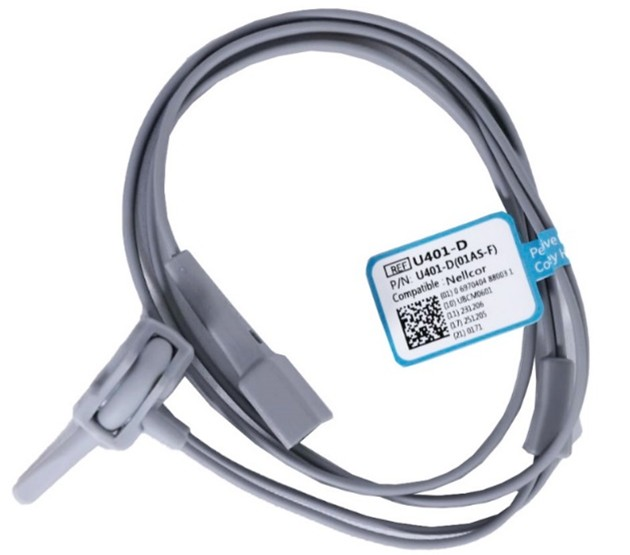
\includegraphics[width=0.5\linewidth]{img/sensor.jpg}
    \caption{Sensor U401-D utilizado para registrar los valores. Fuente: \href{https://www.humanhaim.com/product/sensor-de-oximetria-neo-sp02-7pin-u401-d01as-f/}{HumanHaim.}}
    \label{fig:sensor}
\end{figure}

\newpage

\textbf{PCB de la incubadora}

Contiene el circuito AFE4490 y un microcontrolador ESP32. El AFE es el encargado de amplificar, filtrar y digitalizar las señales analógicas provenientes del sensor óptico, mientras que el microcontrolador gestiona la comunicación con el exterior y la ejecución del firmware.

\begin{figure}[H]
    \centering
    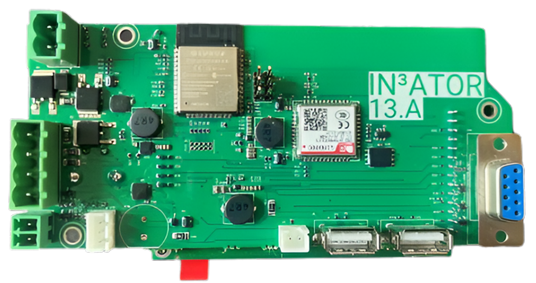
\includegraphics[width=0.75\linewidth]{img/PCB.png}
    \caption{Placa electrónica de la incubadora \textit{In$^3$ator}. \textit{Elaboración propia.}}
    \label{fig:PCB}
\end{figure}

    
\textbf{Programador EPS-Prog}

Permite cargar el firmware en el microcontrolador a través de un puerto de programación. Se conecta al ordenador mediante un adaptador micro-USB.

\begin{figure}[H]
    \centering
    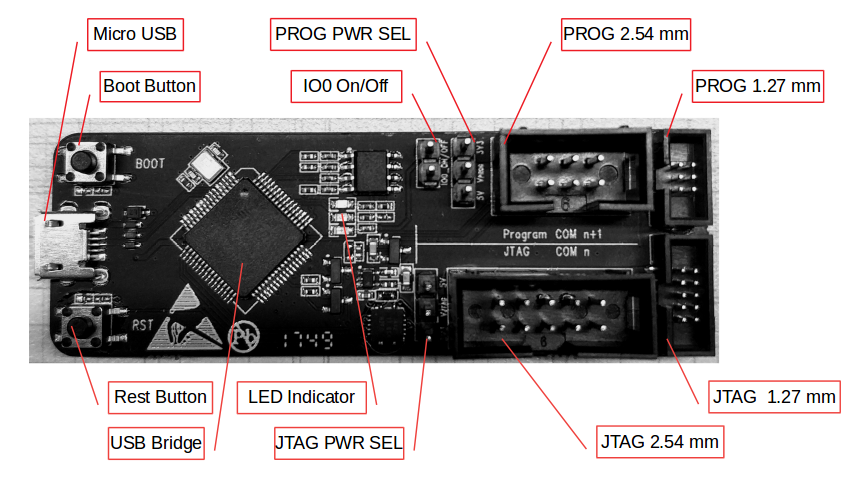
\includegraphics[width=0.7\linewidth]{img/EPS-prog.png}
    \caption{Programador a través del cual se transmiten los datos desde la placa al ordenador. Fuente: \href{https://docs.espressif.com/projects/esp-dev-kits/en/latest/other/esp-prog/user_guide.html}{Espressif.}}
    \label{fig:EPS-prog}
\end{figure}

\newpage

\textbf{Pulsioxímetros comerciales externos}

Utilizados como referencia para validar los resultados del sistema desarrollado:
    \begin{itemize}
        \item \textbf{AOJ-70C Berrcom (Amazon)}
        \begin{figure}[H]
            \centering
            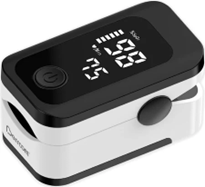
\includegraphics[width=0.3\linewidth]{img/pulsi1.png}
            \caption{Pulsioxímetro comercial 1 para validar los datos. Fuente: \href{https://www.amazon.es/}{Amazon.}}
            \label{fig:pulsi1}
        \end{figure}
        \item \textbf{VitalControl (LIDL)}
        \begin{figure}[H]
            \centering
            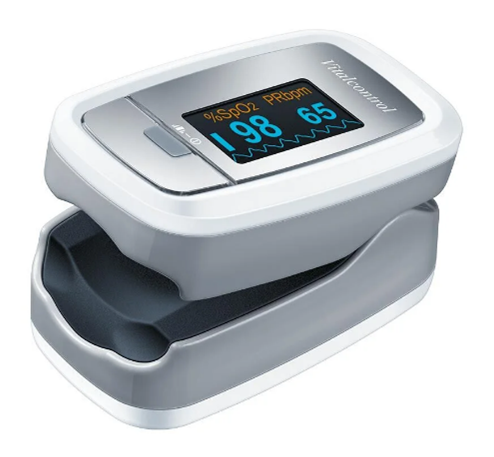
\includegraphics[width=0.35\linewidth]{img/pulsi2.png}
            \caption{Pulsioxímetro comercial 2 para validar los datos. Fuente: \href{https://www.amazon.es/}{Amazon.}}
            \label{fig:pulsi2}
        \end{figure}
    \end{itemize}


\subsubsection{Montaje del sistema}

\begin{enumerate}
    \item Se conecta la fuente de alimentación de 12V a un enchufe doméstico y se acopla un adaptador AC/DC, que convierte la corriente alterna en continua. Este se conecta a la entrada de alimentación de la PCB (ir al punto de conexión 1 de la imagen \ref{fig:PCBpartes}).
    \item El programador EPS-Prog se conecta al ordenador por USB y al microcontrolador en la PCB a través de los pines de programación(ir al punto de conexión 2 de la imagen \ref{fig:PCBpartes}). Una vez detectado por el portátil, permite cargar el firmware mediante PlatformIO.
    \item El sensor óptico U401-D se conecta a la PCB a través de un conector DB9 hembra (ir al punto de conexión 3 de la imagen \ref{fig:PCBpartes}). Durante las mediciones, se fija al dedo del usuario para asegurar un contacto adecuado con la piel.
    \begin{figure}[H]
        \centering
        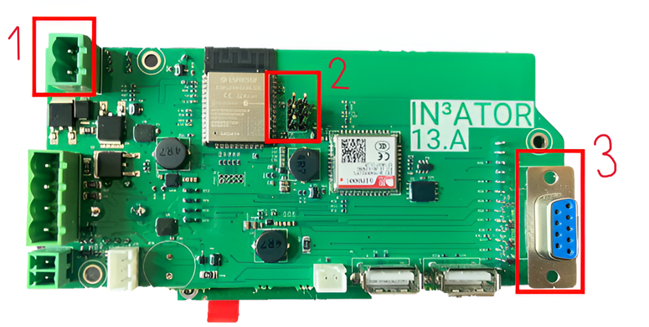
\includegraphics[width=0.85\linewidth]{img/PCBpartes.png}
        \caption{Partes de la PCB que se han utilizado para este proyecto concreto. \textit{Elaboración propia.}}
        \label{fig:PCBpartes}
    \end{figure}
    \item En la otra mano (o en otro dedo de la misma mano), se coloca un pulsioxímetro comercial. Sus lecturas se utilizan como referencia para registrar los valores de SpO$_2$ y frecuencia cardíaca en el nombre del archivo generado: \texttt{raw\_data\_SpO2\_HR.csv}.
\end{enumerate}

\begin{figure}[H]
    \centering
    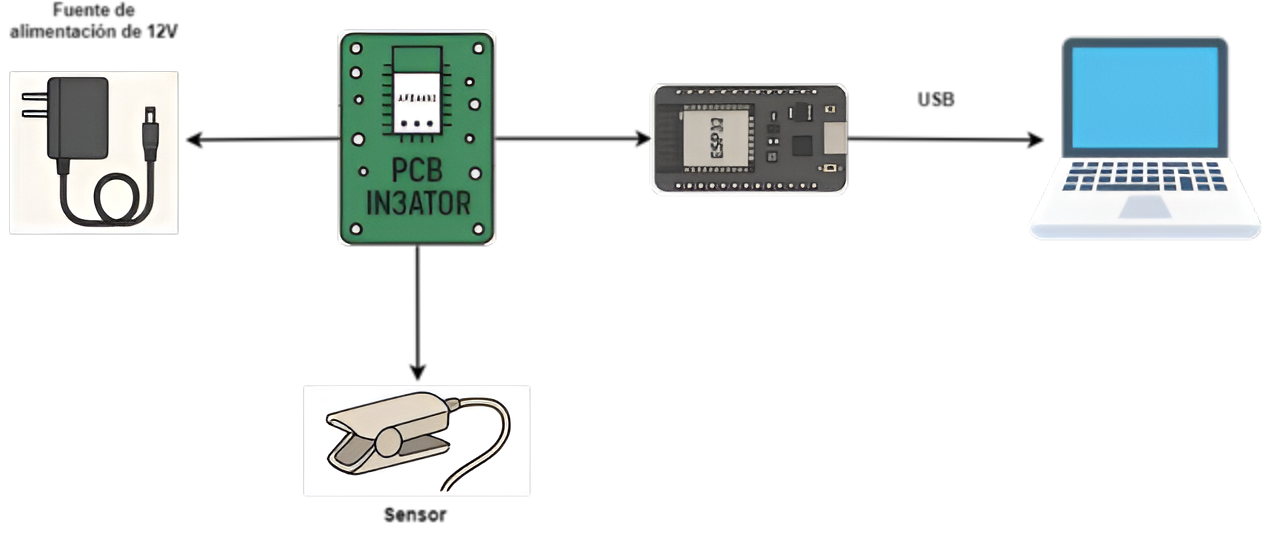
\includegraphics[width=0.95\linewidth]{img/flujo.png}
    \caption{Esquema de conexión para obtener los registros.\textit{Elaboración propia.}}
    \label{fig:flujo}
\end{figure}

\subsection{Software y lenguajes de programación}

Para la adquisición, análisis de los datos e implementación del código, se emplearon las siguientes herramientas de software:

\paragraph{Lenguajes utilizados}

\begin{itemize}
    \item \textbf{Python}: empleado para analizar los logs (registros), procesar las señales PPG y probar los algoritmos de estimación de los parámetros. 
    \item \textbf{C ++}: usado para desarrollar y modificar el firmware que corre en el microcontrolador.
    \item \textbf{LaTeX}: utilizado para la redacción de la memoria del TFG y los anexos técnicos, permitiendo una presentación adecuada.
\end{itemize}

\paragraph{Entornos de desarrollo}

\begin{itemize}
    \item \textbf{Jupyter Notebook}: entorno interactivo para el análisis exploratorio de datos, visualización y documentación del proceso.
    \item \textbf{Visual Studio Code}: entorno de desarrollo principal para trabajar con el firmware. 
\end{itemize}


\paragraph{Librerías de Python}\footnote{Cabe destacar que muchas de las librerías integradas en el entorno de desarrollo original (como PlatformIO en VS Code) ya estaban presentes en el firmware heredado del proyecto, por lo que no todas han sido incorporadas específicamente como parte de este trabajo. Se mencionan aquellas utilizadas en Python.}

\begin{itemize}
    \item \texttt{NumPy}, \texttt{Pandas}: para la manipulación de datos en formato CSV.
    \item \texttt{Matplotlib}, \texttt{Seaborn}: para la visualización de señales y tendencias.
    \item \texttt{SciPy}: para aplicar filtros digitales y detectar picos.
    \item \texttt{OpenCV} (en fase de pruebas): para el tratamiento de ruido y procesamiento de señales como si fueran imágenes.
\end{itemize}

\subsection{Otras herramientas empleadas}

\begin{itemize}
    \item \textbf{PlatformIO}: entorno de desarrollo para microcontroladores integrado en VS Code. Automatiza la gestión de bibliotecas, la compilación y la carga de firmware.
    \item \textbf{Drivers del EPS-Prog}: controladores VCP\footnote{Los controladores de puerto COM virtual (VCP) hacen que el dispositivo USB aparezca como un puerto COM adicional disponible para el PC.} necesarios para que el programador sea reconocido como puerto COM.
    \item \textbf{GitHub}: plataforma utilizada para el control de versiones, documentación y almacenamiento de código. Se gestionaron scripts, versiones del firmware, tareas, hitos y documentación asociada del proyecto.
    \item \textbf{Microsoft Word}: empleado durante las fases iniciales del proyecto para la toma de notas, redacción de borradores y estructuración de contenidos antes de pasarlo a LaTeX.
    \item \textbf{Draw.io (diagrams.net)}: utilizado para la creación de diagramas de bloques que representan los algoritmos, y esquemas funcionales que representan el flujo de la metodología y la arquitectura del sistema.

\end{itemize}


\section{Técnicas de procesamiento de señales}

Debido al enfoque del proyecto, se ha considerado necesario dedicar una sección específica a las técnicas de procesamiento de las señales empleadas.

El objetivo principal de este bloque es detallar los métodos aplicados para limpiar, transformar y analizar las señales PPG, así como los criterios seguidos para estimar los parámetros fisiológicos objetivo. A lo largo de esta sección se describen las distintas estrategias exploradas, su validación práctica sobre los datos reales adquiridos y la justificación técnica de las decisiones adoptadas para seleccionar los algoritmos finales.


Antes de proceder al diseño e implementación de los algoritmos de estimación, se realizó una fase de selección de las señales registradas. Con el objetivo de mejorar la precisión del análisis, se escogieron manualmente aquellas adquisiciones que presentaban señales estables, minimizando la presencia de artefactos de movimiento e interferencias lumínicas.\footnote{A pesar de realizar una selección previa, se seguían registrando señales que mostraban artefactos de distintos tipo, pero aun así se analizaron aquellas partes de la señal que podrían ofrecer información valiosa}

El análisis y desarrollo de estos algoritmos se llevó a cabo en Jupyter Notebook, y todos los scripts empleados se encuentran disponibles en el repositorio del proyecto para su consulta y replicación. Esta elección permitió trabajar en un entorno controlado, con el objetivo de experimentar con distintas estrategias de filtrado y estimación sin las limitaciones del microcontrolador.  

\subsection{Estimación de la frecuencia cardíaca}

La frecuencia cardíaca se estimó a partir de las señales PPG procedentes de los datos recogidos, explorando diferentes técnicas de procesamiento temporal y frecuencial. A lo largo de este apartado, se detallan los algoritmos evaluados, su implementación práctica y los criterios que guiaron la selección del método final.

El objetivo era seleccionar el algoritmo que ofreciera el mejor compromiso entre precisión, tolerancia frente al ruido y viabilidad de implementación en el microcontrolador del sistema.

Inicialmente, se visualizaron las señales gráficamente y se implementaron diferentes planteamientos fallidos \footnote{Aquellas pruebas con las que no se obtuvieron buenos resultados, serán nombradas en el \textit{anexo G} y están disponibles en el repositorio en el directorio de \texttt{pruebas} dentro del procesamiento de la frecuencia cardíaca.}.

En la fase posterior, se llevó a cabo una revisión de metodologías aplicadas en la literatura científica. Entre ellas destacan el algoritmo de detección de picos adaptativos \cite{9493400}, basado en el uso de un umbral adaptativo en función del ritmo cardíaco, y el método combinado de cruce de umbral y ventana deslizante descrito en la nota de aplicación de Renesas \cite{renesas2022ob1203}.
A partir de estas referencias, se implementaron y compararon diferentes enfoques en Jupyter Notebook, empleando como base los logs de adquisición propios. Los principales métodos evaluados fueron:


\begin{itemize}
    \item \textbf{AFE4403.ipynb}: basado en el artículo técnico de Texas Instruments sobre el AFE4403 \cite{oak2015how}. Se aplicaron filtros pasa-banda Butterworth y Savitzky-Golay para eliminar ruido y calcular la frecuencia cardíaca por separación entre picos.
    \begin{figure}[H]
        \centering
        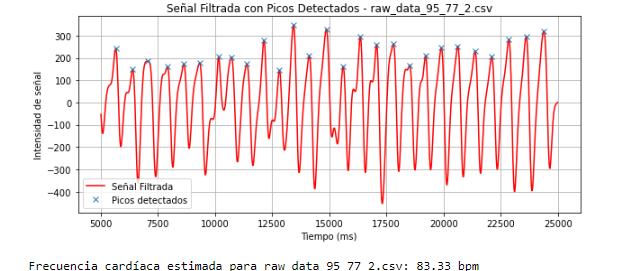
\includegraphics[width=0.85\linewidth]{img/AFE4403.png}
        \caption{Ejemplo de señal filtrada, aplicando el algoritmo del fichero \texttt{AFE4403.ipynb}. \textit{Elaboración propia.}}
        \label{fig:AFE4403}
    \end{figure}
    \item \textbf{AlgoritmoLigero.ipynb}: implementación del algoritmo de Vourvoulakis et al., del artículo \cite{9493400}, basado en umbrales adaptativos sobre las señales IR y RED.
    \begin{figure}[H]
        \centering
        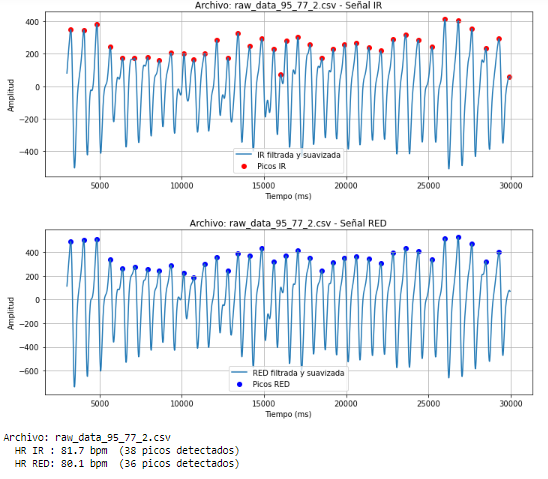
\includegraphics[width=0.85\linewidth]{img/Algoligero.png}
        \caption{Ejemplo de señal filtrada, aplicando el algoritmo del fichero \texttt{AlgoritmoLigero.ipynb}. \textit{Elaboración propia.}}
        \label{fig:AlgoLigero}
    \end{figure}
    \item \textbf{FFT.ipynb}: Este procedimiento no se basa en ningún artículo científico, si no que es un plantemiento que facilita la comprensión del tratamiento de la señal. Se trata de la estimación de la frecuencia cardíaca en el dominio de la frecuencia mediante Transformada Rápida de Fourier tras haber aplicado un filtro paso-bajo.
    \begin{figure}[H]
        \centering
        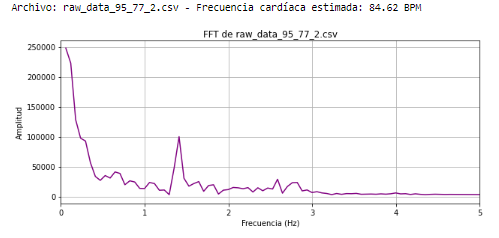
\includegraphics[width=0.85\linewidth]{img/FFT.png}
        \caption{Ejemplo de señal filtrada, aplicando el algoritmo del fichero \texttt{FFT.ipynb}. \textit{Elaboración propia}.}
        \label{fig:FFT}
    \end{figure}
    \item \textbf{procesamiento.ipynb}: procesamiento completo tras eliminación manual de segmentos inestables en los extremos de las señales, se utiliza un filtro Butterworth paso-bajo.
    \begin{figure}[H]
        \centering
        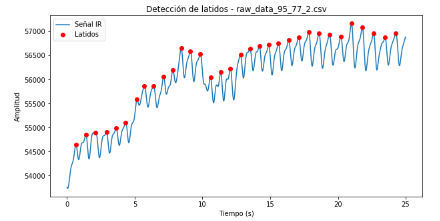
\includegraphics[width=0.85\linewidth]{img/procesamiento.png}
        \label{fig:FFT}
    \end{figure}
    \begin{figure}[H]
        \centering
        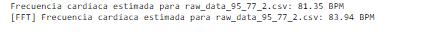
\includegraphics[width=0.85\linewidth]{img/procesamiento1.png}
        \caption{Ejemplo de señal filtrada, aplicando el algoritmo del fichero \texttt{procesamiento.ipynb}. \textit{Elaboración propia}.}
        \label{fig:FFT}
    \end{figure}
    \item \textbf{Pulsi\_comercial.ipynb}: simulación del funcionamiento de un pulsioxímetro comercial, con filtro paso-bajo Butterworth y estimación RR.
    \begin{figure}[H]
        \centering
        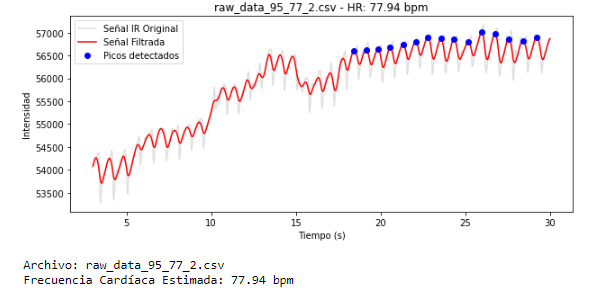
\includegraphics[width=0.85\linewidth]{img/pulsi_comercial.png}
        \caption{Ejemplo de señal filtrada, aplicando el algoritmo del fichero \texttt{pulsi\_comercial.ipynb}. \textit{Elaboración propia}.}
        \label{fig:pulsi_comercial}
    \end{figure}
    \item \textbf{spo2.ipynb}: detección de picos tras filtrado por media móvil y mediana.
    \begin{figure}[H]
        \centering
        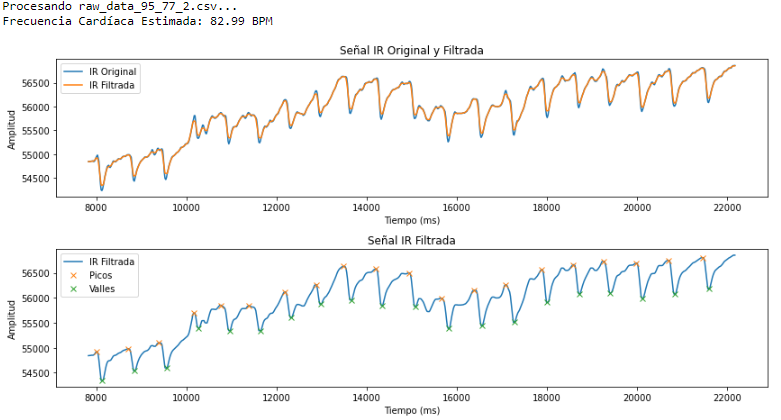
\includegraphics[width=0.75\linewidth]{img/spo2.png}
        \caption{Ejemplo de señal filtrada, aplicando el algoritmo del fichero \texttt{spo2.ipynb}. \textit{Elaboración propia}.}
        \label{fig:spo2}
    \end{figure}
    \item \textbf{temporal\_fft:} Se aplica un filtro pasabanda Butterworth de segundo orden, eliminando componentes de ruido fuera del rango fisiológico del pulso. Posteriormente, se utilizó la transformada rápida de Fourier para identificar la frecuencia dominante del espectro, que se tradujo a pulsaciones por minuto.
    \begin{figure}[H]
        \centering
        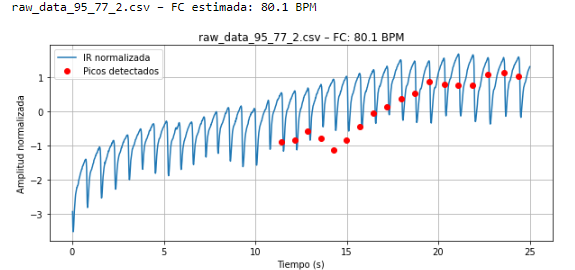
\includegraphics[width=0.85\linewidth]{img/temporal_fft.png}
        \caption{Ejemplo de señal filtrada, aplicando el algoritmo del fichero \texttt{temporal\_fft.ipynb}. \textit{Elaboración propia}.}
        \label{fig:temporal_fft}
    \end{figure}
\end{itemize}

Todas las imágenes mostradas corresponden a un mismo registro. Para ver los resultados de estos algoritmos sobre el resto de logs, consultar los notebooks correspondientes.

\subsubsection{Comparativa de métodos}

De entre todos los métodos analizados, se seleccionaron dos enfoques basados en el dominio temporal para su comparación detallada debido a la precisión de sus resultados:

\begin{enumerate}
    \item Algoritmo basado en media móvil + mediana + detección de picos (\texttt{spo2.ipynb}).
    \item Algoritmo basado en filtro Butterworth + detección de picos y eliminación de outliers (\texttt{pulsi\_comercial.ipynb}).
\end{enumerate}

\paragraph{Método 1: Filtro de media móvil y mediana.}

Este algoritmo se basa en un procesamiento sobre la señal IR corregida. El procedimiento comienza con una limpieza de los extremos del registro para eliminar los primeros y últimos segundos sobrantes (\(t_{\text{inicio}}\), \(t_{\text{fin}}\)) con el objetivo de descartar regiones inestables que puedan contener artefactos asociados al contacto inicial o la retirada del sensor.

\begin{itemize}
    \item La frecuencia de muestreo (\ref{eq:fs}) se estima a partir de la mediana del intervalo temporal (\ref{eq:mediana}) entre muestras consecutivas:
    \begin{equation}
        f_s = \frac{1}{\text{mediana}(\Delta t)} \quad
        \label{eq:fs}
    \end{equation}
    \begin{center}
        donde
    \end{center} \begin{equation}
        \quad \Delta t = \frac{t_{i+1} - t_i}{1000}
        \label{eq:mediana}
    \end{equation}
    \item Se aplica un filtro de media móvil de ventana \(M = 5\) (\ref{eq: media5}) para suavizar oscilaciones no fisiológicas de alta frecuencia:
    \begin{equation}
    IR_{\text{filtrada}}[n] = \frac{1}{5} \sum_{k=-2}^{2} IR[n+k]
    \label{eq: media5}
    \end{equation}
    \item A continuación, se aplica un filtro de mediana con una ventana también de 5 muestras, con el fin de eliminar picos de ruido que podrían confundirse con pulsos reales, conservando la morfología de los pulsos.
    \item La detección de pulsos se realiza a través de un algoritmo de búsqueda de máximos locales. En primer lugar, se identifican los picos como los puntos más altos de la señal filtrada, siempre que cumplan con una separación mínima entre sí. Posteriormente, se obtiene la posición de los valles aplicando el mismo algoritmo sobre la señal invertida (\(-IR_{\text{filtrada}}\)), permitiendo localizar los mínimos locales con el mismo criterio. Para evitar contar múltiples picos dentro de un mismo latido, se impone una distancia mínima de 0.5 segundos (\ref{eq:dist}) entre detecciones consecutivas:

    \begin{equation}
    \text{distancia mínima} = 0.5 \cdot f_s
    \label{eq:dist}
    \end{equation}
    \item Finalmente, se calcula la frecuencia cardíaca (\ref{eq: HR2}) a partir de la media de los intervalos de tiempo entre valles consecutivos:
    \begin{equation}
    HR = \frac{60}{\text{media}(\Delta t_{\text{valles}})}
    \label{eq: HR2}
    \end{equation}
\end{itemize}

\begin{figure}[H]
    \centering
    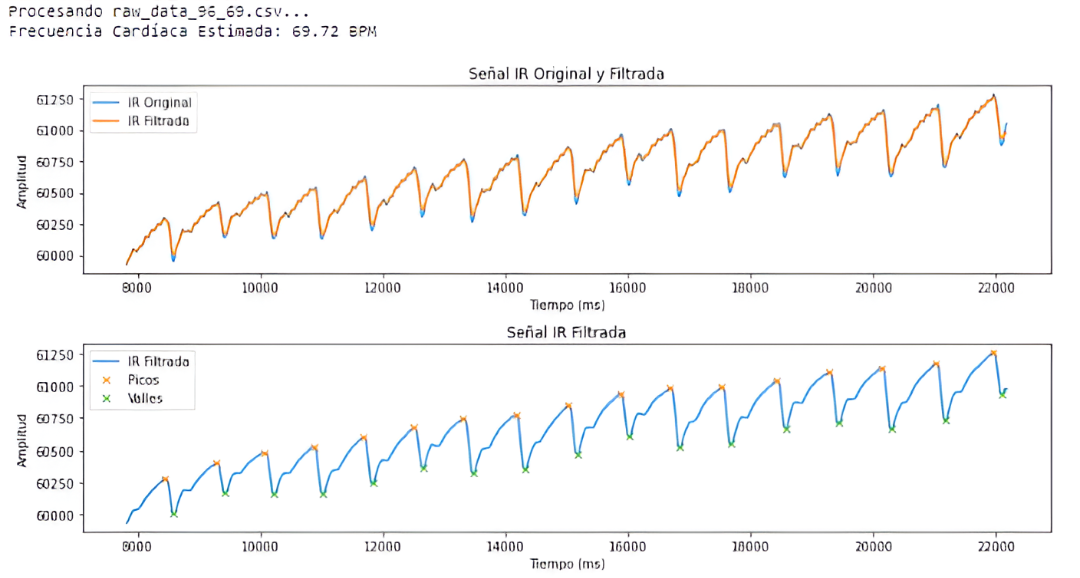
\includegraphics[width=0.95\linewidth]{img/spo2_2.png}
    \caption{Ejemplo de aplicar el algoritmo mencionado sobre otro log diferente. \textit{Elaboración propia.}}
    \label{fig:spo2_2}
\end{figure}

Este método se ha escogido por su eficacia y destaca por su simplicidad y eficiencia computacional, por lo que resulta adecuado para implementarlo más adelante en el firmware original.


\paragraph{Método 2: Filtro Butterworth pasa-bajo y detección de picos con eliminación de outliers.}

Este segundo método se basa en aplicar un filtrado digital suave, seguido de una detección de picos sobre la señal IR.

\begin{itemize}
    \item Se parte de los datos previamente limpiados (archivos CSV en la carpeta \texttt{Datos\_limpios}), con la señal IR.
    \item La señal IR se suaviza utilizando un filtro digital pasa-bajo Butterworth de orden 3 y frecuencia de corte \( f_c = 3{,}5\,\text{Hz} \). El filtrado se aplica en ambos sentidos mediante \texttt{filtfilt}. Este método localiza los máximos locales que cumplen dos condiciones fisiológicas:
\begin{itemize}
    \item Se exige una altura mínima adaptativa (\ref{eq: height}), definida como el percentil 80 de la señal. Esto permite ignorar oscilaciones menores y centrarse solo en los pulsos más elevados:
    \begin{equation}
    \texttt{height} = \text{percentil}_{80}(\text{señal filtrada})
    \label{eq: height}
    \end{equation}
    \item Se impone una separación mínima entre pulsos de 18 muestras, equivalente a 0,18 segundos con un muestreo de 100 Hz. Esto limita la detección a un máximo fisiológico de aproximadamente 333 latidos por minuto:
    \begin{equation}
    \texttt{distance} = 18 \text{ muestras } \Rightarrow HR_{\text{máx}} \approx \frac{60}{0{,}18} \approx 333\,\text{bpm}
    \end{equation}
\end{itemize}
    \item A partir de los picos detectados, se calculan los intervalos RR:
    \begin{equation}
    \Delta t_i = t_{i+1} - t_i
    \end{equation}
    \item Para evitar que errores puntuales afecten al resultado, se eliminan los intervalos entre pulsos RR que se alejan demasiado del comportamiento normal. Para ello, se aplica el criterio del rango intercuartílico (IQR), que descarta los valores demasiado pequeños o demasiado grandes respecto a la mayoría. En lugar de usar el valor típico de 1.5, se ha optado por un umbral más estricto de 1.2, lo que ayuda a reducir falsos positivos en la estimación de la frecuencia cardíaca:
    \begin{equation}
    \Delta t \in [Q_1 - 1{,}2 \cdot IQR,\ Q_3 + 1{,}2 \cdot IQR]
    \end{equation}
    \item Finalmente, se estima la frecuencia cardíaca (\ref{eq:HR3}) a partir del intervalo medio entre picos válidos:
    \begin{equation}
    HR = \frac{60}{\text{media}(\Delta t_{\text{filtrados}})}
    \label{eq:HR3}
    \end{equation}
\end{itemize}

\begin{figure}[H]
    \centering
    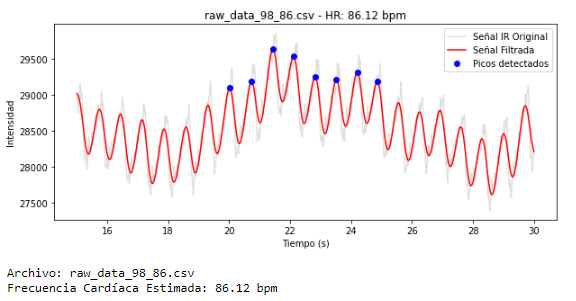
\includegraphics[width=0.85\linewidth]{img/pulsicomercial.png}
    \caption{Aplicación del algoritmo sobre señal real IR. En rojo la señal filtrada, en azul los picos detectados. \textit{Elaboración propia.}}
    \label{fig:pulsicomercial}
\end{figure}

Gracias al filtrado y a la detección adaptativa de picos, este método permite obtener estimaciones bastante fiables de la frecuencia cardíaca. Aun así, algunas de las funciones que utiliza, como \texttt{filtfilt} (para filtrar en ambos sentidos) o el cálculo de percentiles, son difíciles de trasladar tal cual al firmware, ya que habría que programarlas desde cero en C++. 


\paragraph{Selección final:}

Para seleccionar el mejor enfoque, se estudió el tiempo de ejecución de ambos filtros (sobre los logs de 60Hz de frecuencia)\footnote{Se puede revisar esta comprobación dentro del repositorio en el fichero \texttt{benchmark\_filtros.ipynb}, del directorio de procedimiento} y aunque resultó que el de menor tiempo computacional fue el filtro Butterworth, se optó finalmente por el algoritmo basado en filtro de media móvil. Si bien el método Butterworth ofrecía mejor rendimiento ante señales contaminadas, el hecho de utilizar funciones específicas de Python, lo hacía menos adecuado para su implementación en el microcontrolador actual.



\subsection{Estimación de SpO$_2$}

Al igual que en el caso de la frecuencia cardíaca, la estimación de la saturación de oxígeno en sangre requirió una fase exploratoria inicial. En ella se llevaron a cabo pruebas sobre los datos adquiridos, experimentando con técnicas de filtrado, métodos alternativos y ajustes de preprocesamiento. Estas pruebas se documentan en los notebooks correspondientes, disponibles en el repositorio del proyecto.

Los métodos principales considerados para la estimación de SpO$_2$ son los siguientes:

\paragraph{Método 1: \texttt{spo\_algo\_v4.ipynb}, Estimación mediante algoritmo adaptado del firmware.}

Este método representa una de las versiones desarrolladas a partir de la función \texttt{spo2\_algorithm.cpp} incluida en el archivo \texttt{SPO2.cpp} del firmware \textbf{original} de la incubadora. Dicho algoritmo estaba poco optimizado y no era fácilmente validable desde un entorno externo, ya que estaba integrado con el resto del sistema embebido. Por ello, se adaptó su lógica al entorno Python, lo que permitió visualizar sus resultados y validar su comportamiento sobre los datos adquiridos en las pruebas reales.

Aunque el firmware original implementa el cálculo de SpO$_2$ mediante una tabla de búsqueda (LUT, Look-Up-Table), en el propio archivo se encuentra comentada una fórmula alternativa cuadrática (\ref{eq:cuadratica}) que permite estimar la saturación directamente a partir del ratio de absorciones. Esta fórmula es la que se ha empleado en este método por su simplicidad, continuidad y buena aproximación dentro del rango fisiológico normal.

La fórmula:

\begin{equation}
SpO_2 = -45.060 \cdot R^2 + 30.354 \cdot R + 94.845
\label{eq:cuadratica}
\end{equation}

Esta expresión se obtiene a partir de regresiones cuadráticas realizadas sobre datos experimentales. Es decir, se mide el ratio \( R \) de absorción para diferentes personas o simulaciones, y se ajusta una curva que relacione ese ratio con el valor de SpO$_2$ medido por un pulsioxímetro de referencia. El resultado es una fórmula que permite estimar directamente la saturación a partir del ratio sin necesidad de tablas discretas.

El procedimiento aplicado fue el siguiente:

\begin{itemize}
    \item Se parte de los datos crudos adquiridos por el sensor, correspondientes a las intensidades de luz detectadas por los canales IR y RED.
    \item Se calcula la media de cada señal (\ref{eq:media}) para estimar su componente continua o de fondo (DC). Esto equivale a encontrar el nivel base de la señal:
    \begin{equation}
    \text{mean}_{IR} = \overline{IR}, \quad \text{mean}_{RED} = \overline{RED}
    \label{eq:media}
    \end{equation}
    \item A continuación, se resta esa media a cada señal para obtener su componente alterna (\ref{eq:AC}), que representa la parte pulsátil:
    \begin{equation}
    AC_{IR} = IR - \text{mean}_{IR}, \quad AC_{RED} = RED - \text{mean}_{RED}
    \label{eq:AC}
    \end{equation}
    \item Para cuantificar la amplitud de esa señal alterna, se calcula la \textbf{raíz cuadrada media (RMS)} de cada canal:
    \begin{equation}
    RMS_{IR} = \sqrt{\frac{1}{n} \sum_{i=1}^{n} (AC_{IR}[i])^2}, \quad RMS_{RED} = \sqrt{\frac{1}{n} \sum_{i=1}^{n} (AC_{RED}[i])^2}
    \label{eq:RMS}
    \end{equation}
    \item Con esos valores se calcula un ratio que compara la absorción de las dos longitudes de onda:
    \begin{equation}
    R = \frac{RMS_{RED} / \text{mean}_{RED}}{RMS_{IR} / \text{mean}_{IR}}
    \end{equation}
    \item Finalmente, se aplica la fórmula cuadrática ya mencionada para obtener la estimación del valor global de SpO$_2$ en el registro analizado.
\end{itemize}

\begin{figure}[H]
    \centering
    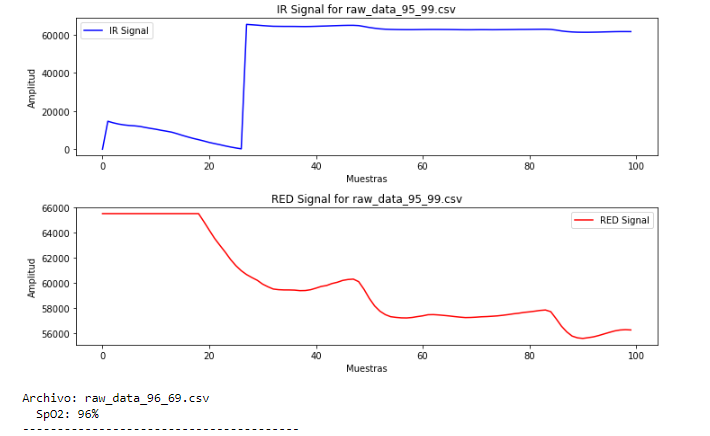
\includegraphics[width=0.85\linewidth]{img/spo2algo.png}
    \caption{Aplicación del algoritmo a los datos crudos según el archivo \texttt{spo\_algo\_v4.ipynb}. \textit{Elaboración propia.}}
    \label{fig:spo2algo}
\end{figure}

Aunque este método resulta sencillo de implementar y computacionalmente eficiente, los resultados obtenidos durante su validación sobre las señales reales del sistema no fueron completamente satisfactorios. En concreto, en algunos registros se observaron desviaciones notables respecto a los valores de referencia, con estimaciones de SpO$_2$ que resultaban poco realistas.

Estas limitaciones pueden deberse a varios factores: la sensibilidad del ratio \( R \) a pequeñas variaciones en la señal, y el uso de una fórmula empírica que no está ajustada específicamente a las condiciones del sensor empleado. Aun así, este método sirvió como base para compararlo con enfoques desarrollados posteriormente.


\paragraph{Método 2: \texttt{tabla\_LUT.ipynb}, Estimación basada en generación de tabla LUT.}

Este segundo método parte de una idea diferente al algoritmo del firmware. En lugar de aplicar directamente una fórmula empírica fija como en el método anterior, aquí se propone construir una tabla LUT personalizada, generada a partir de los datos reales adquiridos durante las pruebas del sistema. El objetivo es observar la relación entre el ratio óptico \(R\) calculado a partir de las señales y el valor de SpO$_2$ que se había registrado con un pulsioxímetro comercial como referencia.

El procedimiento seguido en este notebook fue el siguiente:

\begin{itemize}
    \item Se recorrieron todos los archivos CSV con datos limpios.
    \item Para cada archivo, se cargaron las señales IR y RED, y se calcularon sus componentes AC (desviación típica) y DC (media). Con esos valores se estimó el ratio óptico mediante:
    \begin{equation}
    R = \frac{AC_{RED} / DC_{RED}}{AC_{IR} / DC_{IR}}
    \end{equation}
    \item Se almacenó, para cada archivo, el valor de \(R\) y su correspondiente SpO$_2$ de referencia.
    \begin{figure}[H]
        \centering
        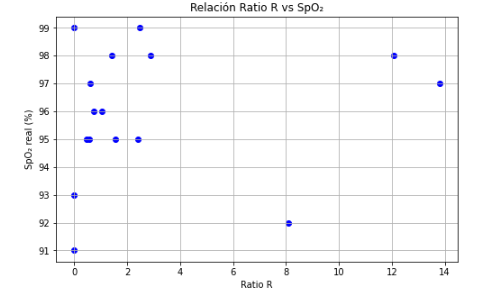
\includegraphics[width=0.75\linewidth]{img/LUT2.png}
        \caption{Gráfico de dispersión que relaciona los valores de R con los de SpO$_2$ a partir del archivo \texttt{tabla\_LUT.ipynb}. \textit{Elaboración propia.}}
        \label{fig:LUT2}
    \end{figure}
    \item Finalmente, se representaron gráficamente estos valores (figura \ref{fig:LUT2}) y se detectaron algunos puntos con ratios extremos (muy altos o iguales a cero). Tras este filtrado, se obtuvo una tabla LUT con pares de valores \((R, \text{SpO}_2)\) válidos, que permite visualizar la tendencia real entre el ratio óptico y la saturación.
    \begin{figure}[H]
        \centering
        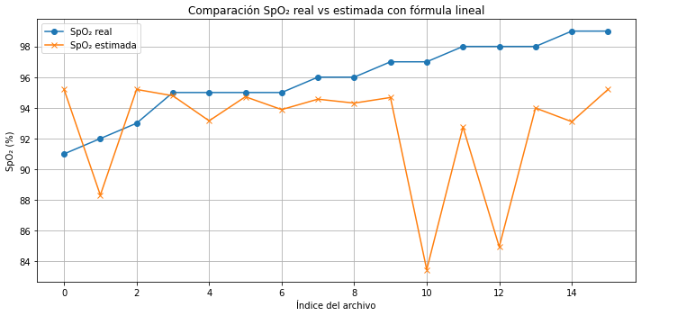
\includegraphics[width=0.85\linewidth]{img/LUT1.png}
        \caption{Comparación de los resultados con los valores de SpO$_2$ de referencia. \textit{Elaboración propia.}}
        \label{fig:LUT1}
    \end{figure}
\end{itemize}

Esta tabla se puede utilizar como base para futuros modelos personalizados (por ejemplo, una regresión lineal o una interpolación), o incluso para crear una LUT discreta implementable en firmware. El enfoque permite adaptar la estimación de SpO$_2$ al comportamiento real del sensor en el sistema desarrollado y tiene la ventaja de apoyarse directamente en datos experimentales propios.

No obstante, durante su ejecución se detectaron varios registros con valores erróneos o inconsistentes (por ejemplo, ratios iguales a cero o superiores a 8), que indican la sensibilidad de este método a errores de adquisición o ruido. También es importante destacar que para que esta opción sea fiable, es necesario tener un mayor número de logs o registros.


\paragraph{Método 3: \texttt{Paper\_CS.ipynb}: Estimación mediante regresión lineal ajustada.}

Este método propone una estrategia basada en aprendizaje automático sencillo: en lugar de utilizar una fórmula empírica genérica o una tabla LUT fija, se ajusta un modelo de regresión lineal personalizado utilizando exclusivamente los datos reales obtenidos durante las pruebas del sistema. Se ha tomado de base un artículo \cite{mohan2010blood}.

La idea es la siguiente: para cada archivo de registro de señales PPG (IR y RED), se calcula el ratio óptico \( R \) a partir del cociente entre las componentes pulsátiles (AC) de ambas señales, corregidas por sus respectivas componentes continuas (DC). La señal se corrige previamente restando la luz ambiental (\texttt{AMB\_IR} y \texttt{AMB\_RED}), y se calcula la RMS (\ref{eq:RMS2}) de las señales corregidas:

\begin{equation}
R = \frac{RMS_{RED}}{RMS_{IR}} \quad \text{donde   }   RMS = \sqrt{\frac{1}{n} \sum_{i=1}^{n} (x[i])^2}
\label{eq:RMS2}
\end{equation}

Luego, se toma como variable dependiente el valor real de SpO$_2$ anotado en el nombre del archivo (medido con un pulsioxímetro comercial) y se entrena un modelo de regresión lineal con la forma:

\begin{equation}
SpO_2 = m \cdot R + b
\end{equation}

Tras el ajuste, se obtuvo el siguiente modelo:

\begin{equation}
SpO_2 = -0.9560 \cdot R + 96.66
\end{equation}

\begin{figure}[H]
    \centering
    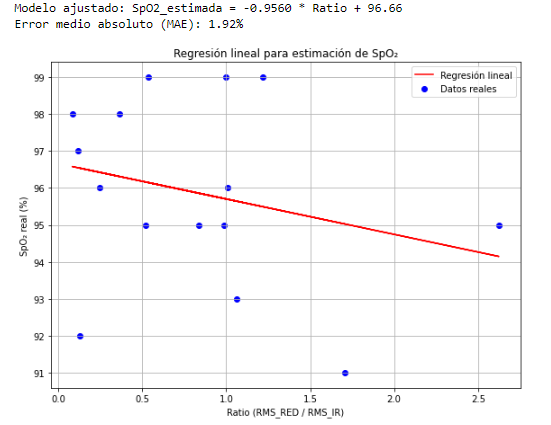
\includegraphics[width=0.75\linewidth]{img/modelo.png}
    \caption{Modelo de regresión obtenido con los datos propios para conseguir los valores \textit{a} y \textit{b} según el archivo \texttt{Paper\_CS.ipynb}. \textit{Elaboración propia.}}
    \label{fig:modelo}
\end{figure}

Este modelo fue validado con los datos disponibles, obteniendo un error medio absoluto (MAE) de 1.92 puntos porcentuales (figura \ref{fig:modelo}), lo que indica una buena capacidad de estimación promedio en las condiciones de adquisición empleadas.


Este método tiene la ventaja de estar ajustado directamente a las características reales del sistema, y permite una implementación sencilla en firmware (como una ecuación lineal). Además, ofrece una interpretación clara: a mayor ratio \( R \), menor saturación estimada, lo cual coincide con el comportamiento fisiológico esperado.

No obstante, es importante señalar que la calidad del ajuste depende fuertemente de la calidad y representatividad de los datos usados. En este caso, el modelo ha sido ajustado únicamente con señales limpias y valores de referencia de un único usuario, por lo que su generalización a otros pacientes o condiciones clínicas no ha sido evaluada.

\paragraph{Método 4: \texttt{uch\_spo2\_table.ipynb}: Generación personalizada de tabla LUT tipo firmware.}

Este método tiene como objetivo replicar el funcionamiento del algoritmo del firmware original, que utiliza una tabla de búsqueda (\texttt{uch\_spo2\_table}) para estimar el valor de SpO$_2$ a partir del ratio óptico \( R \). Sin embargo, en lugar de utilizar la tabla precalibrada incluida en el código fuente, en este caso se genera una LUT personalizada basada en los datos reales adquiridos durante el desarrollo del proyecto.

Este método se diferencia del anterior (basado en una LUT visual) en que, en lugar de almacenar valores de SpO$_2$ para cada índice, busca una expresión matemática directa que relacione el ratio óptico con la saturación.


El proceso seguido fue el siguiente:

\begin{itemize}
    \item Se recorrieron los archivos CSV con datos limpios, en los que el valor de SpO$_2$ real se extraía del nombre del archivo.
    \item Para cada archivo, se calcularon las señales corregidas (\texttt{IR} - \texttt{AMB\_IR} y \texttt{RED} - \texttt{AMB\_RED}), y se obtuvieron sus componentes AC y DC.
    \item Se calculó el ratio óptico como:
    \begin{equation}
    R = \frac{AC_{RED}/DC_{RED}}{AC_{IR}/DC_{IR}}, \quad \text{donde }
    \end{equation}
    \begin{equation}
    AC = \max(\text{señal}) - \min(\text{señal},) \quad DC = \overline{\text{señal}}
    \end{equation}
    \item El valor del ratio se multiplicó por 100 y se redondeó para usarlo como índice de acceso a la tabla LUT.
    \item Para cada índice (de 0 a 183), se almacenaron los valores de SpO$_2$ reales correspondientes, y se calculó su media.
    \item Los índices sin datos suficientes fueron rellenados mediante interpolación lineal, asegurando una tabla continua sin saltos muy grandes. El resultado fue una tabla de 184 posiciones que asigna un valor de SpO$_2$ a cada rango de ratio observado.

\end{itemize}

Esta tabla fue visualizada y validada gráficamente (figura \ref{fig:uch_spo2}), mostrando el comportamiento fisiológico esperado. El método permite estimar directamente el valor de SpO$_2$ de cualquier nuevo registro utilizando una única operación de acceso a tabla (más interpolación si se desea). No obstante, también hereda las limitaciones mencionadas en otros métodos.

\begin{figure}[H]
    \centering
    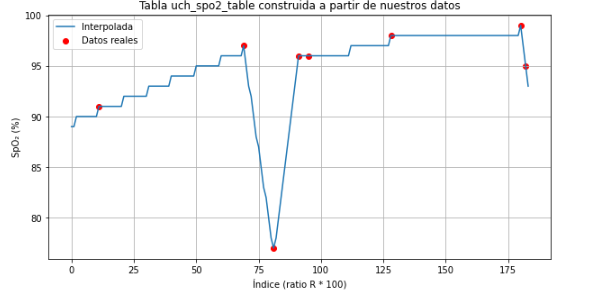
\includegraphics[width=0.85\linewidth]{img/uch_spo2.png}
    \caption{Gráfico de la tabla construida a partir de los datos propios a partir del archivo \texttt{uch\_spo2\_table.ipynb}. \textit{Elaboración propia}.}
    \label{fig:uch_spo2}
\end{figure}


\paragraph{Selección final:}

De entre los métodos evaluados, el que mostró mejor equilibrio entre precisión, estabilidad y viabilidad de implementación en firmware fue el \textbf{Método 4}, basado en una tabla de búsqueda discreta generada a partir de los datos reales adquiridos con el sistema. Este método permitió capturar la relación entre el ratio óptico \(R\) y la saturación de oxígeno SpO$_2$ directamente desde los experimentos realizados, evitando el uso de fórmulas genéricas o calibraciones externas.

Aunque otros enfoques como la fórmula cuadrática (Método 1) o la regresión lineal ajustada (Método 3) ofrecían ventajas en términos de continuidad o simplicidad matemática, el uso de una LUT precalculada resultó menos sensible frente a señales con ruido. Además, la implementación tipo firmware de esta tabla permite estimaciones rápidas y estables sin necesidad de cálculos complejos en tiempo real.

Por tanto, la versión final del firmware emplea este método LUT, lo que asegura una estimación de SpO$_2$ coherente con el comportamiento real del sensor y viable dentro de las limitaciones del sistema.

\vspace{0.4cm}
\noindent
\textbf{Resumen comparativo y criterios de selección}

Más allá de la precisión teórica, la elección del algoritmo final tuvo en cuenta factores como la estabilidad ante ruido y la viabilidad de implementación en sistemas embebidos. En la Tabla~\ref{tab:resumen_spo2} se sintetizan las principales características de cada enfoque probado.

\begin{table}[H]
\centering
\footnotesize
\renewcommand{\arraystretch}{1.2}
\begin{tabular}{|p{2.6cm}|p{4.4cm}|p{4.4cm}|}
\hline
\textbf{Método} & \textbf{Ventajas} & \textbf{Limitaciones} \\
\hline
\textbf{1. Fórmula cuadrática} & Continuo, simple de aplicar & Sensible al ruido, desviaciones fisiológicas \\
\hline
\textbf{2. LUT visual} & Ajustado a datos reales, interpretable & No implementable directamente, requiere muchos datos \\
\hline
\textbf{3. Regresión lineal} & Ecuación directa y calibrable & Dependiente del conjunto de entrenamiento, poco robusto \\
\hline
\rowcolor{gray!20}
\textbf{4. LUT tipo firmware} & Robusto, eficiente, fácil de integrar & Precisión limitada al conjunto de calibración inicial \\
\hline
\end{tabular}
\caption{Resumen de los métodos de estimación de SpO$_2$ evaluados. \textit{Elaboración propia.}}
\label{tab:resumen_spo2}
\end{table}


\subsection{Implementación en el firmware}

Una vez identificados los algoritmos más adecuados para la estimación de la frecuencia cardíaca y la saturación de oxígeno en entorno Python, se procedió a su adaptación al firmware del sistema embebido. Esta etapa supuso un reto técnico importante, ya que implicaba trasladar algoritmos previamente validados en un entorno conocido a un código escrito en un lenguaje poco trabajado durante el grado, y además hacerlo respetando la estructura existente del firmware, con múltiples archivos interdependientes y funciones ya implementadas.

El objetivo era lograr que el microcontrolador fuera capaz de procesar los datos en tiempo real y emitir directamente por puerto serie los valores de frecuencia cardíaca y SpO$_2$, eliminando la necesidad de postprocesamiento en PC. Para ello, fue necesario reestructurar parte del código original, optimizar las funciones de cálculo y rediseñar el flujo de adquisición y salida de datos.

La Figura~\ref{fig:flujo_firmware} muestra el esquema general del nuevo flujo de procesamiento de señal implementado dentro del firmware.


\begin{figure}[H]
    \centering
    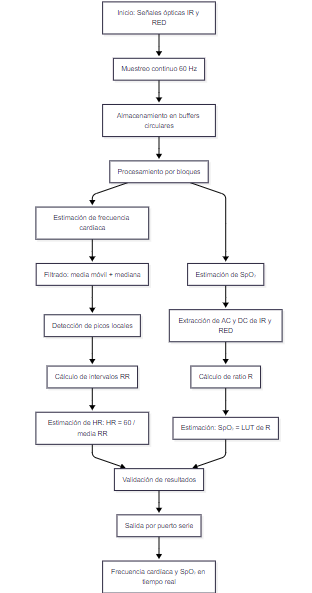
\includegraphics[width=0.6\linewidth]{img/flujo_firmware.png}
    \caption{Diagrama de flujo que representa el código implementado en el firmware. \textit{Elaboración propia.}}
    \label{fig:flujo_firmware}
\end{figure}

\newpage

\paragraph{Estimación de la frecuencia cardíaca.}

La estimación de la frecuencia cardíaca se implementa dentro de la función \texttt{estimate\_spo2()} del archivo \texttt{SPO2.cpp}, que procesa bloques de datos adquiridos por el sensor. El firmware trabaja sobre la señal IR, almacenada en un buffer circular \footnote{Un \textit{buffer circular} es una estructura de datos que almacena una cantidad fija de elementos y, cuando se llena, comienza a sobrescribir los datos más antiguos con los nuevos. Permite procesar continuamente señales, por eso, se suele utilizar en sistemas en tiempo real.}
de 128 posiciones, actualizado en tiempo real a una frecuencia de muestreo de 100 Hz. Esto permite mantener siempre una ventana de datos recientes sin necesidad de desplazar manualmente los elementos del buffer.

La señal IR se centra restando su media y se invierte, de modo que los valles fisiológicos (mínimos de absorción) se transforman en picos. Posteriormente, se suaviza con una media móvil de cuatro muestras, y sobre esa señal invertida se aplica un umbral adaptativo para detectar los picos correspondientes a los valles reales.

\begin{figure}[H]
    \centering
    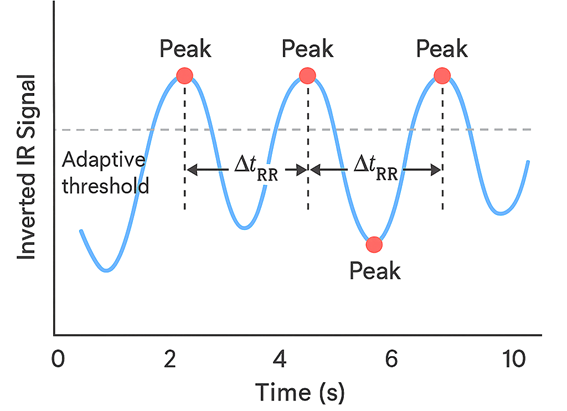
\includegraphics[width=0.5\linewidth]{img/fc_algo.png}
    \caption{Detección de picos locales en una señal pulsátil y cálculo de intervalos RR. \textit{Elaboración propia.}}
    \label{fig:enter-label}
\end{figure}

Si se detectan al menos dos valles válidos, se calcula la frecuencia cardíaca estimando el intervalo medio entre ellos ($\Delta t_{\text{RR}}$), y aplicando la fórmula:

\begin{equation}
\text{HR} = \frac{60}{\text{media}(\Delta t_{\text{RR}})}
\end{equation}

donde:

\begin{equation}
\Delta t_i = \frac{t_{i+1} - t_i}{f_m}
\end{equation}

y $f_m$ es la frecuencia de muestreo en Hz. El resultado final se valida para asegurar que se encuentra dentro del rango fisiológico razonable (entre 40 y 220 BPM). Si no cumple con esta condición, se descarta.


\paragraph{Estimación de la saturación de oxígeno.}

La estimación de SpO$_2$ se realiza en la misma función \texttt{estimate\_spo2()}, reutilizando los valles previamente detectados en la señal IR para dividir la señal en ciclos pulsátiles (es decir, segmentos entre dos latidos consecutivos). En cada ciclo se calcula la componente AC y la componente DC tanto de la señal RED como de la IR, aplicando las siguientes fórmulas:

\begin{equation}
AC = \max(x) - \min(x)\end{equation}\begin{equation} \qquad DC = \max(x)
\end{equation}

Con estos valores se calcula el \textit{ratio óptico} $R$, utilizando la siguiente expresión:

\begin{equation}
R = \frac{AC_{\text{RED}} \cdot DC_{\text{IR}} \cdot 100}{AC_{\text{IR}} \cdot DC_{\text{RED}}}
\end{equation}

Este cálculo se repite para un máximo de cinco ciclos válidos. Un ciclo se considera válido si las componentes AC y DC superan unos umbrales mínimos predefinidos, que garantizan que la señal no esté afectada por ruido o por un mal contacto del sensor.

Una vez obtenidos hasta cinco valores válidos de \(R\), estos se ordenan y se toma la mediana, ya que es menos sensible a valores atípicos provocados por artefactos de movimiento o interferencias.

El sistema emplea una tabla LUT con 184 posiciones. El valor de \(R\) se redondea al entero más próximo y se utiliza como índice para consultar el valor correspondiente de SpO\textsubscript{2} en dicha tabla:


\begin{equation}
\text{SpO}_2 = \text{LUT}[R]
\end{equation}

El valor estimado se valida asegurando que se encuentra dentro del rango fisiológico razonable (85\,\%–100\,\%); en caso contrario, se descarta.




\capitulo{5}{Resultados}

Este capítulo recoge los principales resultados obtenidos tras todo el proceso de desarrollo, pruebas y validación del sistema. Aunque desde el inicio no se aspiraba a desarrollar un sistema perfecto ni definitivo, el objetivo ha sido lograr una primera versión funcional que sirviera como base para futuras mejoras.

Implementar un pulsioxímetro real, que funcione sobre un sistema embebido, con señales reales, no ha sido una tarea sencilla. A lo largo del proyecto ha habido muchas dificultades, desde la adquisición de datos fiables hasta la adaptación de los algoritmos al firmware. Aun así, se ha conseguido desarrollar un sistema capaz de estimar en tiempo real tanto la frecuencia cardíaca como la saturación de oxígeno, y mostrar esos valores de forma continua con una frecuencia y precisión aceptables.

El sistema todavía tiene un gran margen de mejora, sobre todo en lo que respecta a la estimación de la SpO\textsubscript{2}, que ha resultado más sensible y compleja de ajustar. Sin embargo, el hecho de haber llegado a una implementación completa que funciona sobre el microcontrolador y ofrece resultados coherentes ya supone un avance importante.

A continuación, se presentan los resultados obtenidos en cada fase: primero en entorno Python, donde se probaron distintos algoritmos, y después en el firmware, donde se validó la funcionalidad final en tiempo real.

\subsection{Resumen de los resultados de la estimación de frecuencia cardiaca con Python}

En la Figura~\ref{fig:comparacion_fc_algoritmos} se presenta una comparativa visual de los resultados obtenidos al aplicar este procesamiento sobre los datos crudos del pulsioxímetro, donde se calculan los valores estimados de frecuencia cardíaca siguiendo la metodología previamente descrita:

\begin{figure}[H]
    \centering
    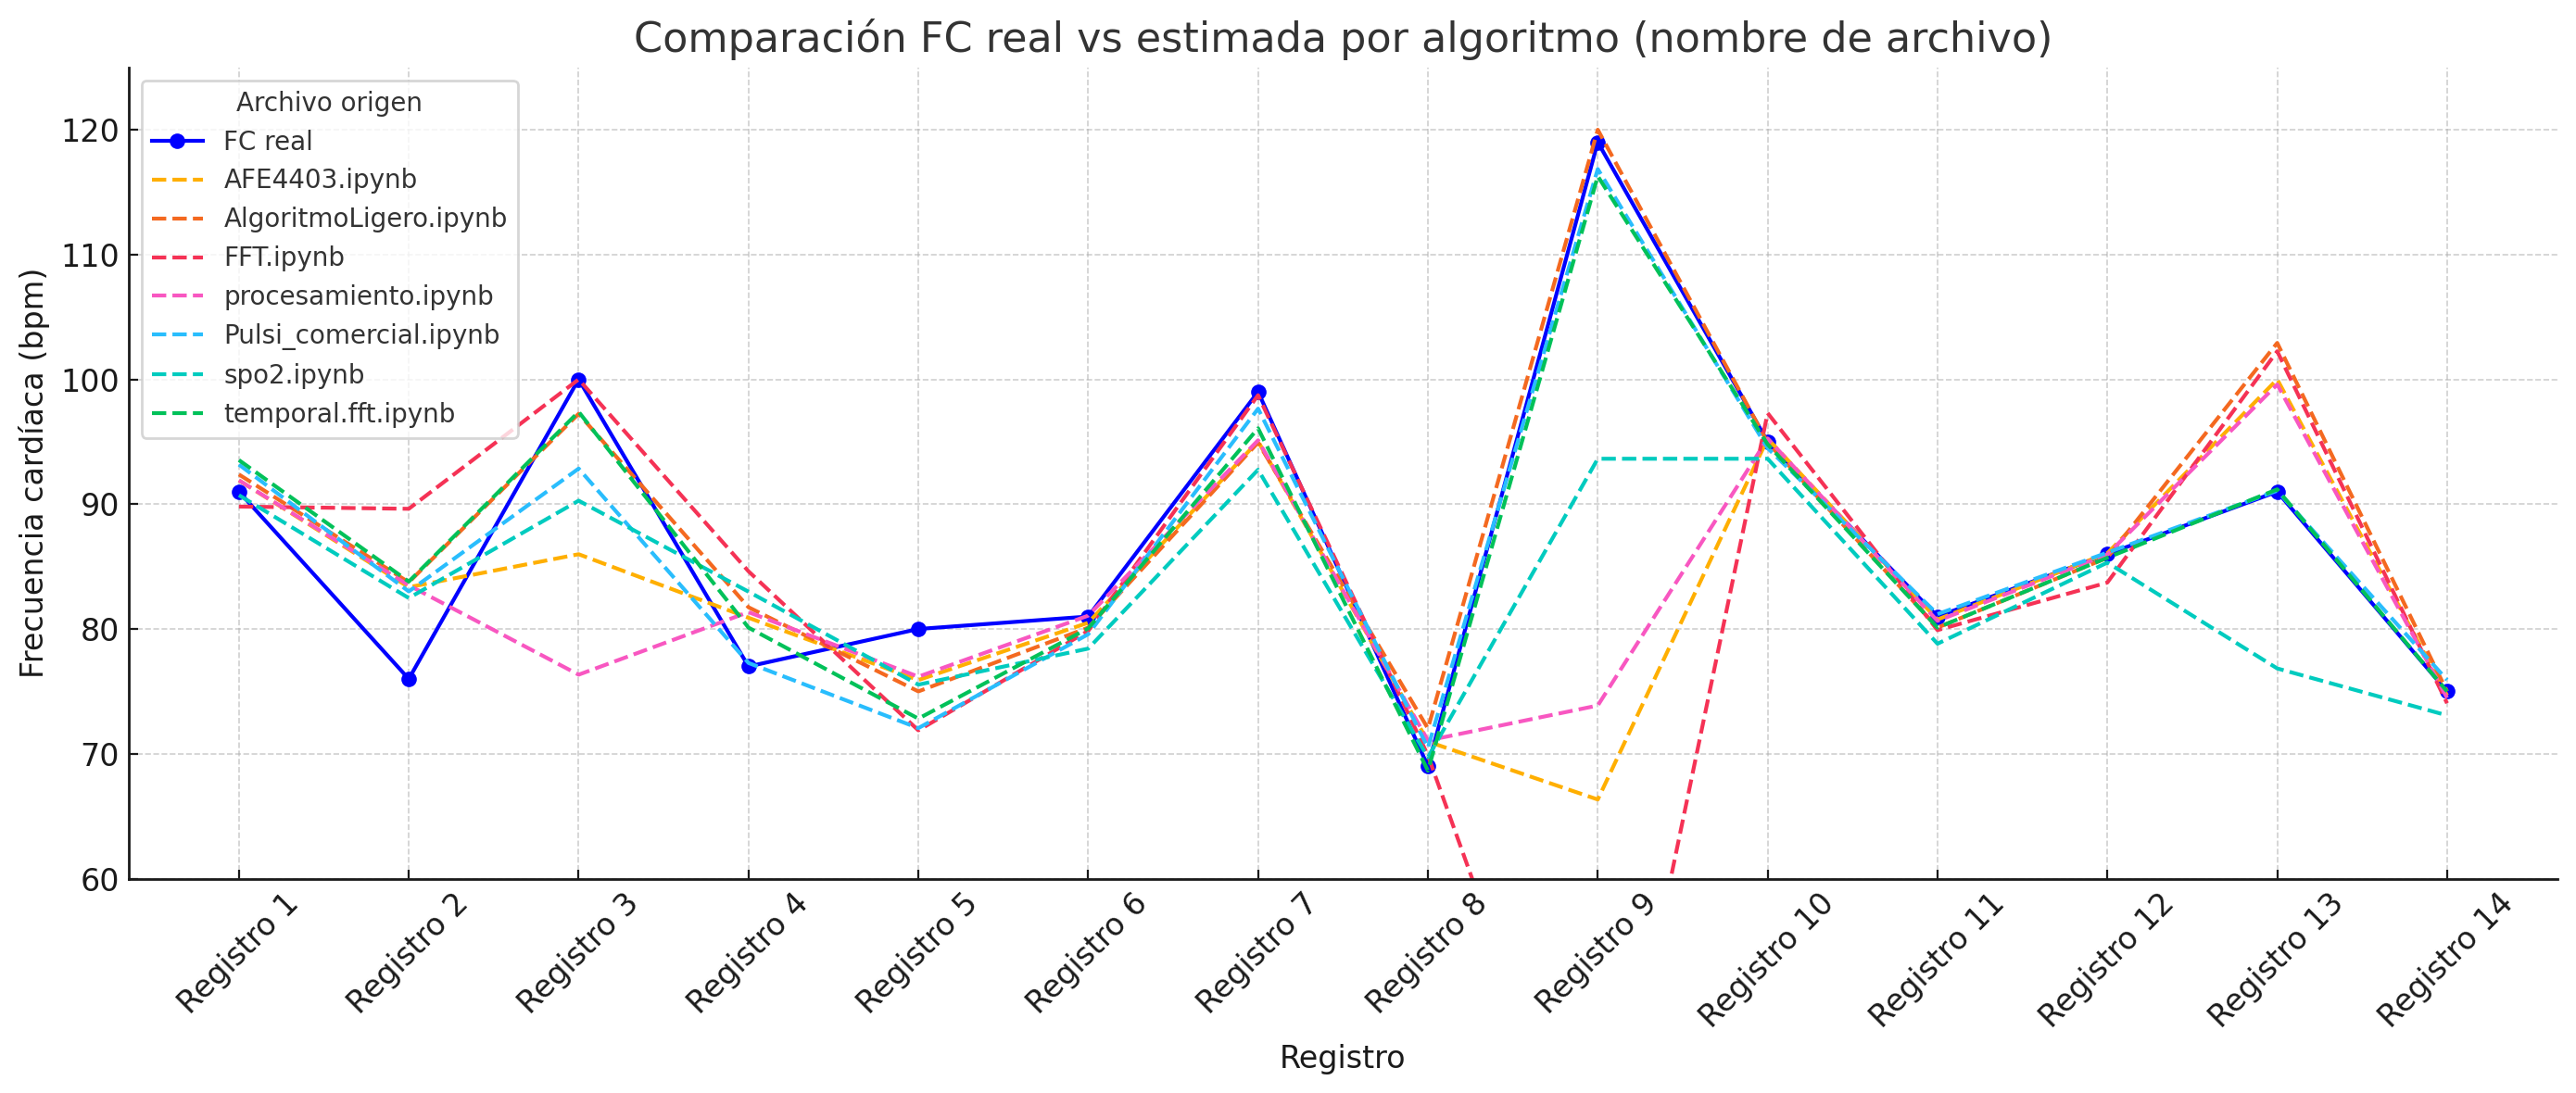
\includegraphics[width=1\linewidth]{img/calculo_fc.png}
    \caption{Gráfica comparativa entre entre la frecuencia cardíaca real y las frecuencias estimadas. \textit{Elaboración propia.}}
    \label{fig:comparacion_fc_algoritmos}
\end{figure}

A continuación se recogen los resultados detallados en forma tabular para cada uno de los métodos evaluados:


%\vspace{-1em} 

\begin{table}[H]
\centering
\begin{tabular}{|c|c|c|}
\hline
\textbf{FC esperada (bpm)} & \textbf{FC calculada (bpm)} & \textbf{Error relativo (\%)} \\
\hline
91 & 91.91 & 1.00 \\
\hline
76 & 83.35 & 9.67 \\
\hline
100 & 85.99 & 14.01 \\
\hline
77 & 80.90 & 5.06 \\
\hline
80 & 75.91 & 5.11 \\
\hline
81 & 80.50 & 0.62 \\
\hline
99 & 95.04 & 4.00 \\
\hline
106 & 77.17 & 27.20 \\
\hline
69 & 70.98 & 2.87 \\
\hline
119 & 66.34 & 44.25 \\
\hline
95 & 95.25 & 0.26 \\
\hline
81 & 80.76 & 0.30 \\
\hline
86 & 86.07 & 0.08 \\
\hline
91 & 100.00 & 9.89 \\
\hline
75 & 74.67 & 0.44 \\
\hline
91 & 82.55 & 9.29 \\
\hline
\end{tabular}
\caption{Error relativo (\%) entre FC esperada y calculada tras aplicar filtro Butterworth, correspondiente al archivo \texttt{AFE4403.ipynb.}}
\label{tabla:fc_afe4403_error_relativo}
\end{table}



\begin{table}[H]
\centering
\resizebox{\textwidth}{!}{%
\begin{tabular}{|c|c|c|c|c|}
\hline
\textbf{FC esperada (bpm)} & \textbf{HR IR (bpm)} & \textbf{HR RED (bpm)} & \textbf{Error IR (\%)} & \textbf{Error RED (\%)} \\
\hline
91 & 92.38 & 70.59 & 1.52 & 22.45 \\
\hline
76 & 83.74 & 82.87 & 10.18 & 9.04 \\
\hline
100 & 97.24 & 73.53 & 2.76 & 26.47 \\
\hline
77 & 81.74 & 80.11 & 6.16 & 4.04 \\
\hline
80 & 75.00 & 75.00 & 6.25 & 6.25 \\
\hline
81 & 80.11 & 80.11 & 1.10 & 1.10 \\
\hline
99 & 94.94 & 94.94 & 4.10 & 4.10 \\
\hline
106 & 100.08 & 94.94 & 5.59 & 10.53 \\
\hline
69 & 72.03 & 72.03 & 4.39 & 4.39 \\
\hline
119 & 120.00 & 120.24 & 0.84 & 1.04 \\
\hline
95 & 94.94 & 94.94 & 0.06 & 0.06 \\
\hline
81 & 80.11 & 80.11 & 1.10 & 1.10 \\
\hline
86 & 85.71 & 85.84 & 0.34 & 0.19 \\
\hline
91 & 102.92 & 102.92 & 13.09 & 13.09 \\
\hline
75 & 75.00 & 73.53 & 0.00 & 1.96 \\
\hline
91 & 81.86 & 66.67 & 10.06 & 26.75 \\
\hline
\end{tabular}%
}
\caption{Error relativo (\%) entre FC esperada y HR calculadas, correspondiente al archivo \texttt{AlgoritmoLigero.ipynb}.}
\label{tabla:fc_algoritmo_ligero_error_relativo}
\end{table}



\begin{table}[H]
\centering
\resizebox{\textwidth}{!}{%
\begin{tabular}{|c|c|c|}
\hline
\textbf{FC esperada (bpm)} & \textbf{FC estimada (bpm)} & \textbf{Error relativo (\%)} \\
\hline
91 & 89.81 & 1.31 \\
\hline
76 & 89.63 & 17.93 \\
\hline
100 & 100.00 & 0.00 \\
\hline
77 & 84.62 & 9.90 \\
\hline
80 & 71.88 & 10.15 \\
\hline
81 & 79.85 & 1.42 \\
\hline
99 & 98.73 & 0.27 \\
\hline
106 & 30.00 & 71.70 \\
\hline
69 & 69.87 & 1.26 \\
\hline
119 & 31.96 & 73.14 \\
\hline
95 & 97.30 & 2.42 \\
\hline
81 & 79.91 & 1.35 \\
\hline
86 & 83.72 & 2.65 \\
\hline
91 & 102.25 & 12.36 \\
\hline
75 & 74.05 & 1.27 \\
\hline
\end{tabular}%
}
\caption{Error relativo (\%) entre FC esperada y FC estimada tras representar la señal en forma FFT, correspondiente al archivo \texttt{FFT.ipynb.}}
\label{tabla:fc_fft_error_relativo}
\end{table}


\begin{table}[htbp]
\centering
\resizebox{\textwidth}{!}{%
\begin{tabular}{|c|c|c|}
\hline
\textbf{FC esperada (bpm)} & \textbf{FC estimada (bpm)} & \textbf{Error relativo (\%)} \\
\hline
91 & 91.91 & 1.00 \\
\hline
76 & 83.50 & 9.87 \\
\hline
100 & 76.34 & 23.66 \\
\hline
77 & 81.35 & 5.65 \\
\hline
80 & 76.18 & 4.77 \\
\hline
81 & 81.07 & 0.09 \\
\hline
99 & 95.12 & 3.92 \\
\hline
106 & 66.77 & 37.01 \\
\hline
69 & 71.07 & 3.00 \\
\hline
119 & 73.87 & 37.92 \\
\hline
95 & 95.25 & 0.26 \\
\hline
81 & 80.65 & 0.43 \\
\hline
86 & 85.97 & 0.03 \\
\hline
91 & 99.59 & 9.44 \\
\hline
75 & 74.48 & 0.69 \\
\hline
91 & 82.05 & 9.84 \\
\hline
\end{tabular}%
}
\caption{Error relativo (\%) entre FC esperada y FC estimada tras aplicar filtro Butterworth paso bajo y FFT, correspondiente al archivo \texttt{procesamiento.ipynb}.}
\label{tabla:fc_procesamiento_error_relativo}
\end{table}


\begin{table}[htbp]
\centering
\resizebox{\textwidth}{!}{%
\begin{tabular}{|c|c|c|}
\hline
\textbf{FC esperada (bpm)} & \textbf{FC estimada (bpm)} & \textbf{Error relativo (\%)} \\
\hline
91 & 93.17 & 2.38 \\
\hline
76 & 83.01 & 9.22 \\
\hline
100 & 92.85 & 7.15 \\
\hline
77 & 77.28 & 0.36 \\
\hline
80 & 72.06 & 9.92 \\
\hline
81 & 79.58 & 1.75 \\
\hline
99 & 97.65 & 1.36 \\
\hline
106 & 105.98 & 0.02 \\
\hline
69 & 70.49 & 2.16 \\
\hline
119 & 116.85 & 1.81 \\
\hline
95 & 94.49 & 0.54 \\
\hline
81 & 81.19 & 0.23 \\
\hline
86 & 86.12 & 0.14 \\
\hline
91 & 91.08 & 0.09 \\
\hline
75 & 75.92 & 1.23 \\
\hline
91 & 82.82 & 8.99 \\
\hline
\end{tabular}%
}
\caption{Error relativo (\%) entre FC esperada y FC estimada tras aplicar filtro Butterworth pasa-banda, correspondiente al archivo \texttt{Pulsi\_comercial.ipynb}}
\label{tabla:fc_pulsioximetro_comercial_error_relativo}
\end{table}


\begin{table}[H]
\centering
\resizebox{\textwidth}{!}{%
\begin{tabular}{|c|c|c|}
\hline
\textbf{FC esperada (bpm)} & \textbf{FC estimada (bpm)} & \textbf{Error relativo (\%)} \\
\hline
91 & 90.72 & 0.31 \\
\hline
76 & 82.48 & 8.53 \\
\hline
100 & 90.28 & 9.72 \\
\hline
77 & 82.99 & 7.78 \\
\hline
80 & 75.54 & 5.57 \\
\hline
81 & 78.43 & 3.17 \\
\hline
99 & 92.76 & 6.30 \\
\hline
69 & 69.72 & 1.04 \\
\hline
95 & 93.64 & 1.43 \\
\hline
81 & 78.82 & 2.69 \\
\hline
86 & 85.32 & 0.79 \\
\hline
75 & 73.08 & 2.56 \\
\hline
91 & 76.84 & 15.56 \\
\hline
\end{tabular}%
}
\caption{Error relativo (\%) entre FC esperada y FC estimada tras aplicar filtro de media y mediana, correspondiente al archivo \texttt{spo2.ipynb}.}
\label{tabla:fc_media_mediana_error_relativo}
\end{table}



\begin{table}[H]
\centering
\resizebox{\textwidth}{!}{%
\begin{tabular}{|c|c|c|}
\hline
\textbf{FC esperada (bpm)} & \textbf{FC estimada (bpm)} & \textbf{Error relativo (\%)} \\
\hline
91 & 93.53 & 2.78 \\
\hline
76 & 83.80 & 10.26 \\
\hline
100 & 97.40 & 2.60 \\
\hline
77 & 80.11 & 4.04 \\
\hline
80 & 72.82 & 8.98 \\
\hline
81 & 80.05 & 1.17 \\
\hline
99 & 96.08 & 2.95 \\
\hline
106 & 103.09 & 2.75 \\
\hline
69 & 68.65 & 0.51 \\
\hline
119 & 116.28 & 2.29 \\
\hline
95 & 94.79 & 0.22 \\
\hline
81 & 80.11 & 1.10 \\
\hline
86 & 85.71 & 0.34 \\
\hline
91 & 91.19 & 0.21 \\
\hline
75 & 75.00 & 0.00 \\
\hline
91 & 80.11 & 11.97 \\
\hline
\end{tabular}%
}
\caption{Estimación de frecuencia cardíaca con error relativo corregido, correspondiente al archivo \texttt{temporal\_fft.ipynb.}}
\label{tabla:fc_temporal_fft_error}
\end{table}



La frecuencia cardíaca estimada por los algoritmos aplicados tiene un error medio absoluto inferior a 5 BPM en la mayoría de los casos, lo que indica un comportamiento fiable.

Como se ha explicado en la metodología, el método que resultó más viable para ser implementado en el firmware fue el doble filtro de media móvil + mediana, por su optimización y simplicidad, además de ser uno de los procedimientos que mejores resultados obtiene.

\subsection{Resumen resultados de la estimación de la SpO$_2$ con Python}

A diferencia de la frecuencia cardíaca, la estimación de la SpO\textsubscript{2} ha resultado más complicada. Esto se debe a que su rango es más pequeño (normalmente entre 90 y 100\,\%) y cualquier pequeño error en las señales afecta mucho más al resultado final. Además, es un parámetro que depende de la relación entre dos señales (IR y RED), lo que lo hace más sensible a ruido o diferencias de amplitud.

Aunque en Python se han podido probar distintas fórmulas y enfoques, los resultados no han sido tan cercanos al valor real como los que se obtuvieron para la estimación de la frecuencia cardíaca (en la mayoría de los casos). Por este motivo, se trabajó directamente esta parte en el firmware, adaptando el algoritmo a las limitaciones reales del sistema, con el objetivo de asegurar una estimación fiable en tiempo real.

En las siguientes tablas se presentan los resultados obtenidos al aplicar diferentes métodos de estimación de la SpO\textsubscript{2} a los archivos de señal registrados durante el proyecto. Para cada uno de ellos se compara el valor estimado con el valor de referencia extraído del nombre del archivo.

Las estimaciones se han realizado utilizando los enfoques explicados en la sección \ref{cap: Metodología}: desde fórmulas empíricas, hasta métodos más simples como la regresión lineal o el uso de tablas LUT. También se ha incluido un cálculo del error asociado, cuando ha sido posible. Además, se ha intentado que quede más claro con gráficas que enfrentan los valores reales frente a los estimados por cada algoritmo.


\begin{table}[H]
\centering
\begin{tabular}{|c|c|c|}
\hline
\textbf{SpO\textsubscript{2} real (\%)} & \textbf{SpO\textsubscript{2} estimada (\%)} & \textbf{Error (\%)} \\
\hline
91 & 95 & 4 \\
\hline
92 & 95 & 3 \\
\hline
93 & 96 & 3 \\
\hline
95 & 97 & 2 \\
\hline
95 & 99 & 4 \\
\hline
95 & 98 & 3 \\
\hline
95 & 98 & 3 \\
\hline
96 & 96 & 0 \\
\hline
96 & 99 & 3 \\
\hline
97 & 0 & 97 \\
\hline
98 & 96 & 2 \\
\hline
98 & 90 & 8 \\
\hline
99 & 95 & 4 \\
\hline
99 & 97 & 2 \\
\hline
99 & 95 & 4 \\
\hline
\end{tabular}
\caption{Comparativa entre la SpO\textsubscript{2} esperada y estimada a partir de los archivos de señal. Archivo de referencia: \texttt{spo\_algo\_v4.ipynb.}}
\label{tabla:spo2_validacion_maxim}
\end{table}

\begin{figure}[H]
    \centering
    
\includegraphics[width=0.95\linewidth]{img/grafico_spo_algo_v4.png}
    \caption{Saturación esperada vs Saturación calculada. Archivo de referencia: \texttt{spo\_algo\_v4.ipynb.}}
    \label{fig:grafico_spo_algo_v4}
\end{figure}


\begin{table}[H]
\centering
\begin{tabular}{|c|c|c|}
\hline
\textbf{SpO\textsubscript{2} real (\%)} & \textbf{Ratio R} & \textbf{SpO\textsubscript{2} estimada (\%)} \\
\hline
91 & 0.000000 & 95.20 \\
\hline
92 & 8.099103 & 88.32 \\
\hline
93 & 0.000000 & 95.20 \\
\hline
95 & 2.484700 & 94.79 \\
\hline
95 & 2.403625 & 93.16 \\
\hline
95 & 0.561102 & 94.72 \\
\hline
95 & 1.543552 & 93.89 \\
\hline
96 & 0.745609 & 94.57 \\
\hline
96 & 1.046738 & 94.31 \\
\hline
97 & 0.617578 & 94.68 \\
\hline
97 & 13.812844 & 83.46 \\
\hline
98 & 2.875030 & 92.75 \\
\hline
98 & 12.062808 & 84.94 \\
\hline
98 & 1.424948 & 94.00 \\
\hline
99 & 2.470356 & 93.10 \\
\hline
99 & 0.000000 & 95.20 \\
\hline
\end{tabular}
\caption{Estimación de SpO\textsubscript{2} mediante fórmula lineal (95.20 - 0.85 · R).\\
Archivo de referencia: \texttt{tabla\_LUT.ipynb.}}

\label{tabla:spo2_formula_lineal}
\end{table}

\begin{figure}[H]
    \centering
    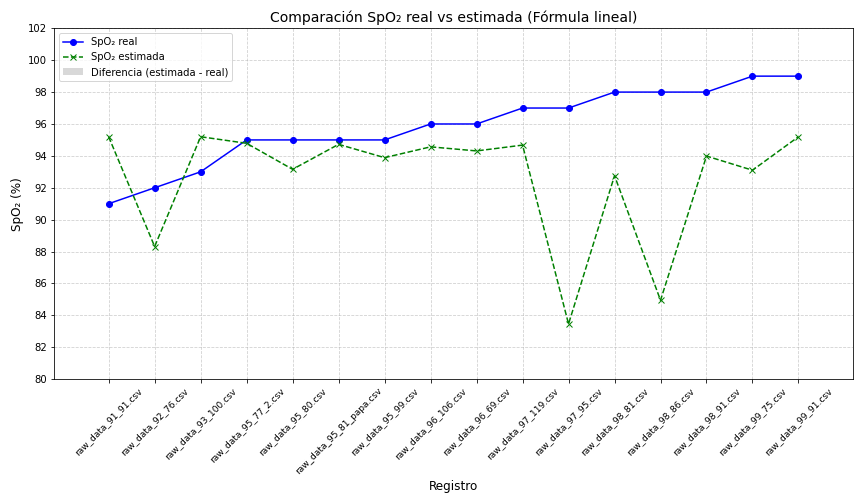
\includegraphics[width=0.95\linewidth]{img/grafico_tabla_LUT.png}
    \caption{Saturación esperada vs Saturación calculada. Archivo de referencia: Archivo de referencia: \texttt{tabla\_LUT.ipynb.}}
    \label{fig:grafico_spo2_lut}
\end{figure}


\begin{table}[H]
\centering
\begin{tabular}{|c|c|c|c|}
\hline
\textbf{SpO\textsubscript{2} real (\%)} & \textbf{SpO\textsubscript{2} estimado medio (\%)} & \textbf{Error (\%)} \\
\hline
91.0 & 95.26 & 4.26 \\
\hline
 92.0 & 96.74 & 4.74 \\
 \hline
93.0 & 96.72 & 3.72 \\
\hline
95.0 & 95.92 & 0.92 \\
\hline
95.0 & 96.36 & 1.36 \\
\hline
95.0 & 94.35 & 0.65 \\
\hline
 95.0 & 96.06 & 1.06 \\
 \hline
 96.0 & 95.97 & 0.03 \\
 \hline
96.0 & 95.89 & 0.11 \\
\hline
97.0 & 95.81 & 1.19 \\
\hline
97.0 & 96.79 & 0.21 \\
\hline
98.0 & 96.52 & 1.48 \\
\hline
98.0 & 96.78 & 1.22 \\
\hline
98.0 & 96.24 & 1.76 \\
\hline
99.0 & 95.35 & 2.65 \\
\hline
99.0 & 95.54 & 3.46 \\
\hline
\end{tabular}
\caption{Comparativa de SpO\textsubscript{2} real, estimación media y error medio. Archivo de referencia: \texttt{Paper\_CS.ipynb}}
\label{tabla:spo2_error_medio}
\end{table}

\begin{figure}[H]
    \centering
    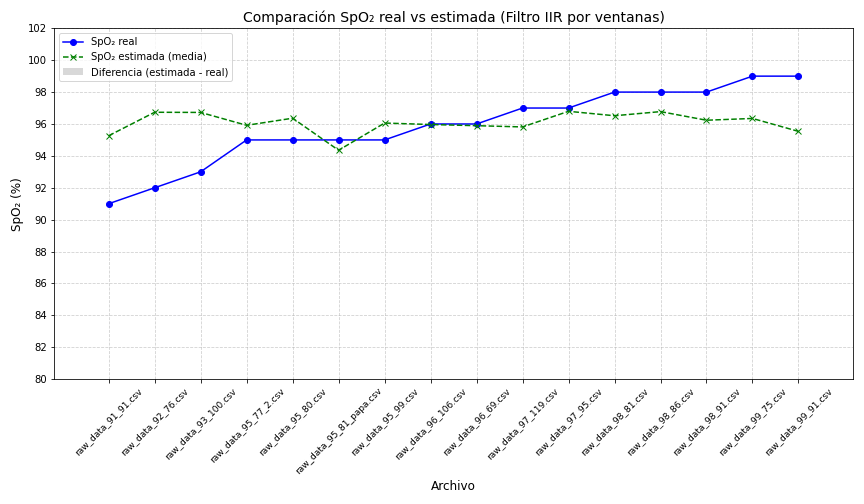
\includegraphics[width=0.95\linewidth]{img/grafico_Paper_CS.png}
    \caption{Saturación esperada vs Saturación calculada. Archivo de referencia: Archivo de referencia: \texttt{Paper\_CS.ipynb.}}
    \label{fig:grafico_Paper_CS}
\end{figure}


\begin{table}[H]
\centering
\begin{tabular}{|l|c|c|c|c|}
\hline
\textbf{SpO\textsubscript{2} real (\%)} & \textbf{Ratio R} & \textbf{SpO\textsubscript{2} estimada (\%)} & \textbf{Error (\%)} \\
\hline
91 & 0.117 & 91 & 0 \\
\hline
92 & 11.906 & 93 & 1 \\
\hline
95 & 0.816 & 77 & 18 \\
\hline
95 & 2.604 & 93 & 2 \\
\hline
95 & 0.538 & 95 & 0 \\
\hline
95 & 1.826 & 95 & 0 \\
\hline
96 & 0.957 & 93 & 3 \\
\hline
96 & 0.912 & 96 & 0 \\
\hline
97 & 0.695 & 97 & 0 \\
\hline
97 & 16.143 & 93 & 4 \\
\hline
98 & 4.252 & 93 & 5 \\
\hline
98 & 1.287 & 98 & 0 \\
\hline
99 & 2.312 & 93 & 6 \\
\hline
99 & 1.805 & 99 & 0 \\
\hline
\end{tabular}
\caption{Estimación de SpO\textsubscript{2} a partir del ratio R, extraída de los archivos de registro. Archivo de referencia: \texttt{uch\_spo2\_table.ipynb.}}
\label{tabla:spo2_ratio_r}
\end{table}

\begin{figure}[H]
    \centering
    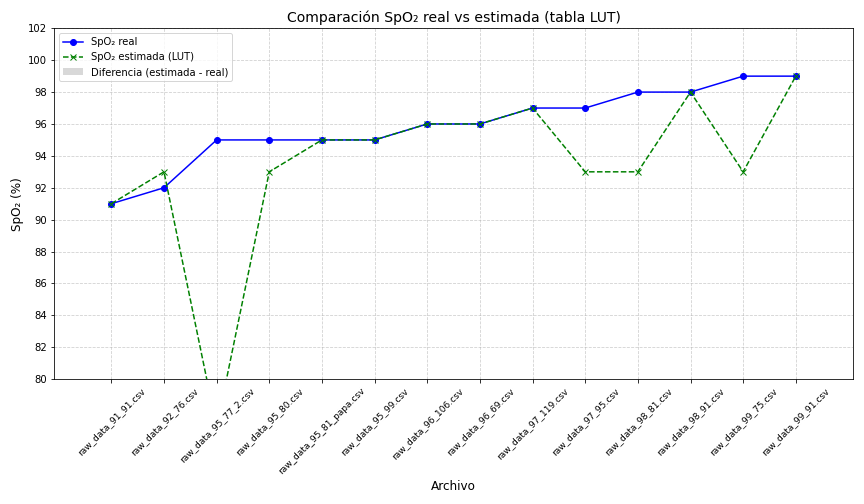
\includegraphics[width=0.95\linewidth]{img/grafico_spo2_lut.png}
    \caption{Saturación esperada vs Saturación calculada. Archivo de referencia: Archivo de referencia: \texttt{uch\_spo2\_tableipynb.}}
    \label{fig:grafico_spo2_lut}
\end{figure}

En el firmware se ha implementado un único algoritmo de estimación de SpO\textsubscript{2}, basado en el método del \textit{Ratio of Ratios} y el uso de una tabla LUT predefinida, que coincide con el implementado en el archivo \texttt{uch\_spo2\_table.ipynb}. Este enfoque fue seleccionado por su simplicidad computacional, bajo coste de recursos y facilidad de adaptación al entorno embebido.



\subsection{Resumen de los resultado de los algoritmos seleccionados en el firmware}

Integrados los algoritmos seleccionados en el firmware, el siguiente paso fue comprobar si realmente funcionaban como se esperaba al ejecutarse directamente sobre el microcontrolador\footnote{A diferencia de la metodología y resultados explicados en el entorno Python, que partían de los datos crudos en formato csv, el firmware recoge los datos que registra el sensor en tiempo real.}. En esta fase, el objetivo ya no es explicar cómo se ha hecho la adaptación (algo que ya se detalla en la metodología), sino observar el comportamiento del sistema en tiempo real y validar que los resultados obtenidos sean coherentes con los que se habían obtenido previamente en las pruebas realizadas en Python.

Para ello, se ejecutó el sistema completo en la placa y se observó la salida por consola, verificando que tanto la frecuencia cardíaca como la SpO\textsubscript{2} se estimaban de forma continua, sin bloqueos y con valores lo más parecidos posible a los mostrados por un pulsioxímetro de referencia con el que se mide al mismo tiempo. 

En la figura \ref{fig:firmware_resultados} se muestran ejemplos reales de la salida del sistema en funcionamiento. En cada línea se informa de la frecuencia cardíaca detectada y del valor de SpO\textsubscript{2} estimado. Como se puede apreciar, los valores se mantienen dentro de un rango fisiológicamente válido, y en muchos casos coinciden con los valores medidos manualmente mediante el sistema de referencia.

\begin{figure}[H]
\centering
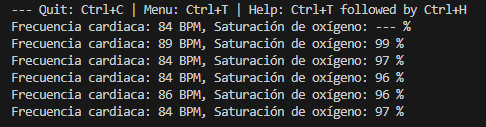
\includegraphics[width=0.8\textwidth]{img/Captura_firmware.png}
\caption{Salida por consola del firmware con los valores estimados de frecuencia cardíaca y SpO\textsubscript{2}. En ese momento se marcaba en el pulsioxímetro comercial un valor de 86 BPM y 98\% de SpO$_2$.}
\label{fig:firmware_resultados}
\end{figure}

En algunos casos puntuales se obtiene un valor de SpO\textsubscript{2} indicado como ``---'', lo cual se debe a que la señal en ese momento no cumplía con los criterios de validación definidos para evitar estimaciones erróneas. El sistema es muy sensible a la luz y al movimiento, como ya se ha mencionado a lo largo de la memoria; por ello, obtener mediciones válidas es complicado. También hay que tener en cuenta que en la mayoría de los casos, los valores indicados como ``---''se deben a que el sistema todavía tiene que estabilizarse.


Además de la captura mostrada, se ha grabado un breve vídeo \footnote{Disponible en el repositorio del proyecto, en el directorio de \texttt{Demostraciones.}} donde se puede ver en tiempo real cómo funciona el sistema al estar conectado a la placa. En él se muestra cómo, tras unos segundos de estabilización, el pulsioxímetro comienza a mostrar valores actualizados de frecuencia cardíaca y SpO \textsubscript{2} por la terminal de VSCode. Este vídeo tiene como objetivo ilustrar visualmente el funcionamiento final del sistema y demostrar que la estimación se realiza de forma continua, en tiempo real, y con una salida estable que responde a los datos recogidos por el sensor.

En conjunto, estos resultados indican que el sistema es capaz de estimar en tiempo real los parámetros fisiológicos de interés, y que los algoritmos seleccionados funcionan de forma coherente en el entorno embebido, respetando las limitaciones de recursos del microcontrolador y manteniéndose dentro de un margen razonable de precisión.


\section{Discusión.}

El resultado final del sistema es una salida en tiempo real que muestra por consola los valores estimados de frecuencia cardíaca y saturación de oxígeno. Como se puede ver en la figura \ref{fig:firmware_resultados}, el sistema es capaz de ofrecer estos datos de manera continua y estable, con valores que entran dentro de los rangos fisiológicamente esperados y que, en la mayoría de los casos, se aproximan bastante a los mostrados por un pulsioxímetro comercial usado como referencia.

Este comportamiento confirma que el sistema no solo es capaz de adquirir y procesar señales reales fsin necesidad de recurrir a procesamiento posterior en un ordenador. A nivel práctico, esto implica que el pulsioxímetro se podría usar directamente en la incubadora, sin depender de equipamiento adicional.

En los entornos hospitalarios avanzados, las incubadoras no suelen integrar el pulsioxímetro como parte del sistema base. Lo habitual es que se conecte un monitor multiparamétrico externo, que incluye otros sensores además del de SpO\textsubscript{2}, y que se coloca al neonato mediante una pinza o parche adhesivo. En cambio, la solución desarrollada en este proyecto está pensada para estar integrada físicamente en la incubadora \textit{In$^3$ator}, y mostrar sus valores de forma conjunta con otros parámetros que ya se controlaban anteriormente, como la temperatura o la humedad. 

Respecto a la comparación con sistemas existentes, es evidente que el prototipo desarrollado no puede competir con la precisión ni la estabilidad de pulsioxímetros comerciales o sistemas que actualmente se emplean en entornos para los que está pensado el trabajo. Sin embargo, eso no quita que se puedan sacar conclusiones interesantes sobre su rendimiento, sobre todo si lo comparamos con otros prototipos más parecidos en objetivos y contexto.

La mayoría de los proyectos mencionados en la sección de conceptos teóricos se centran en fases previas al uso embebido: analizan señales offline, simulan el comportamiento de los sensores o muestran gráficas en Matlab o Python. Por ejemplo, el trabajo de Olga Jiménez\cite{jimenez2019pulsioximetro} desarrolla una interfaz gráfica para la monitorización de constantes, pero el procesado no se integra en un sistema físico. De forma parecida, en el proyecto de Francisco González Romero\cite{gonzalez2019pulsioximetro}, en el que se trabaja con adquisición de señales reales y análisis en entorno PC, pero no se llega a integrar el sistema completo en firmware.

En el caso del trabajo de Jorge Alarcó, de la Universidad Politécnica de Madrid \cite{Alarco2015} sí se llega a validar un sistema real, pero su objetivo está más centrado en la comparación de exactitud frente a modelos certificados, y no en la integración funcional en un entorno concreto como una incubadora.

En cambio, este proyecto ha apostado por una solución pensada para incorporarse desde el diseño al producto final. Esto implica tener en cuenta no solo el rendimiento técnico del algoritmo, sino también la facilidad de fabricación, consumo de recursos y fiabilidad del funcionamiento. El hecho de que los valores de frecuencia cardíaca y SpO\textsubscript{2} se puedan calcular, filtrar y mostrar directamente en pantalla, usando únicamente el microcontrolador y un sensor óptico, supone un paso importante hacia una solución más autónoma y accesible.



\capitulo{6}{Conclusiones}

Desde que comencé este proyecto, he tenido muy presente que se trataba de una oportunidad real para contribuir, aunque fuera en una pequeña parte, a mejorar la calidad asistencial de recién nacidos prematuros en contextos vulnerables. El objetivo inicial era ambicioso: dotar a una incubadora de bajo coste de un sistema funcional de pulsioximetría, capaz de estimar en tiempo real la frecuencia cardíaca y la saturación de oxígeno. Sin embargo, con el paso de las semanas, ese objetivo se fue transformando en un reto que ha abarcado desde la fisiología neonatal y el procesamiento de señales biomédicas, hasta la programación embebida y la validación práctica sobre datos reales.

En este trabajo se ha investigado a fondo el funcionamiento interno de la pulsioximetría y su aplicabilidad al sistema que se planteaba. Se han analizado diferentes técnicas de filtrado y estimación de parámetros fisiológicos, implementándolas en Python y posteriormente adaptándolas al software original de la incubadora. También se ha tenido en cuenta la eficiencia computacional, la estabilidad de las señales y la necesidad de garantizar resultados estables a pesar del ruido que este tipo de sensores ocasiona. El diseño del sistema ha seguido una filosofía de código abierto y bajo coste, sin renunciar a la precisión de los resultados.

Como resultado, se ha conseguido una primera versión funcional del sistema, capaz de registrar y procesar señales PPG en tiempo real, generar una estimación de la frecuencia cardíaca y la SpO$_2$ que, si bien aún presentan limitaciones, sienta un punto de partida sobre el que seguir mejorando. 

Se ha desarrollado una técnica para almacenar y filtrar registros; se ha documentado todo el proceso de desarrollo en un repositorio y se ha validado experimentalmente la viabilidad del enfoque propuesto.

A lo largo de este proceso, también he tomado conciencia de la enorme diferencia que puede suponer una implementación bien pensada en un contexto de bajos recursos. Si algo me llevo de este trabajo, más allá del conocimiento técnico, es la convicción de que la ingeniería aplicada a la salud debe estar al servicio de las personas, especialmente cuando los medios son limitados. Porque diseñar un dispositivo para este tipo de contextos implica centrarse en lo esencial: que funcione, pueda reproducirse y responda a su finalidad.

\section{Aspectos relevantes.}

En líneas generales, se han podido cumplir los objetivos propuestos. Se
han conseguido crear los algoritmos capaces de traducir las señales PPG crudas de un sensor a valores fisiológicos legibles e interpretables por un humano. Sin embargo, a lo largo del desarrollo de este proyecto, han surgido múltiples decisiones técnicas, dificultades prácticas y aprendizajes que han influido directamente en el resultado final. 

Este apartado pretende recoger de los hitos más importantes, justificando los caminos tomados y resaltando aquellos aspectos que podrían resultar útiles para futuros desarrollos similares.

\begin{itemize}
\item \textbf{Inicio del proyecto y contextualización:} El punto de partida fue entender la realidad clínica y social que motiva el proyecto: mejorar el cuidado neonatal en países en vías de desarrollo mediante tecnologías de bajo coste. Esta necesidad guió todas las decisiones posteriores, tanto a nivel de hardware como de software, reforzando el enfoque práctico del sistema.
\item \textbf{Comprensión del entorno de desarrollo:} Uno de los primeros retos fue entender el funcionamiento del sistema de adquisición de señales, así como su configuración. Tanto el lenguaje de programación C++, como el uso de herramientas específicas como PlatformIO, Visual Studio Code o el uso de un programador que transfiriera los datos desde la PCB, eran prácticamente nuevos para mí. Esto supuso una fase inicial de adaptación, en la que fue necesario invertir tiempo en entender cómo funcionaba la arquitectura del sistema, cómo compilar el código y dónde modificar el código base para conseguir el objetivo final, sin apenas referencias previas.

Además, hay que destacar que, aunque el TFG se centra en el desarrollo del sistema de pulsioximetría, este componente está integrado dentro del sistema completo de la incubadora neonatal. Esto conllevó tener que comprender y trabajar sobre una base de código grande, cuyas modificaciones suponen un coste y tiempo computacional considerables, lo que añadió un nivel adicional de complejidad a cada cambio realizado. 

Igualmente, la primera adquisición y visualización de datos tardó más de la cuenta en suceder porque se dieron una serie de problemas técnicos que tenían que ser resueltos en un laboratorio con la ayuda del tutor. En cuanto al hardware, hubo que soldar los pines con los que el programador se conecta con la placa, ya que recibimos el material sin este ajuste realizado. Asimismo, fue necesario probar la ejecución del firmware con varios cables micro-USB porque los que disponíamos no eran reconocidos por el ordenador, y por último, la clavija del programador tuvo que ser apretada para que hiciera buen contacto. En cuanto al software, se tuvo que volver a desplegar el proyecto entero una segunda vez porque al ser tan grande, desde la ruta donde se había alojado inicialmente no se podía ejecutar.

Todos los detalles sobre la puesta en marcha del sistema completo, y las adaptaciones que se realizaron, serán detalladas en el \textit{anexo G}, en el \textit{Cuaderno de Trabajo}.

\item \textbf{Desarrollo del sistema de adquisición y almacenamiento de datos:} Al comienzo, no se sabía lo que el sistema iba a devolver, y al lograr visualizarlo, se observó que iba a ser complicado trabajar directamente en el entorno del firmware y que era necesario exportar estos datos para poder trabajar con ellos de manera independiente. 

Como ya se ha explicado, los datos consistían en la intensidad de las señales IR y RED de los LED del sensor, que si se graficaban frente al tiempo, dan como resultado una señal PPG. El primer inconveniente fue la falta de una referencia temporal de cada registro, y la frecuencia era demasiado elevada, lo que hacía imposible poder trabajar con los datos directamente. Se identificó la función específica del firmware responsable del envío de datos a la terminal con el formato observado y se diseñó un sistema que permitiera capturar datos crudos durante un periodo de 30 segundos, guardarlos en formato CSV e incluir una cabecera que aportara información sobre las señales registradas. 

Esta parte del proyecto facilitó el tratamiento de los datos sin necesidad de realizar modificaciones constantes en el firmware ni de mantener la placa conectada de forma continua.

\item \textbf{Validación experimental:} Se llevaron a cabo sesiones de adquisición de señales con los valores fisiológicos propios de la autora del proyecto en distintas situaciones. Una parte importante del trabajo fue clasificar registros válidos e inválidos, cortar tramos ruidosos y aplicar transformadas de Fourier para estudiar la componente espectral de las señales. Estos análisis permitieron afinar mejor los parámetros de los filtros y del algoritmo de estimación.

Cabe destacar que no se ha podido validar el sistema con recién nacidos prematuros ni en situaciones clínicas reales, por lo que se desconoce si el rendimiento observado en adultos sanos se mantendría en estos pacientes. La frecuencia cardíaca de los recién nacidos prematuros es significativamente más alta que la de un adulto, y en las sesiones de prueba no se pudo elevar la frecuencia cardíaca lo suficiente como para simular este escenario. Además, el sensor empleado es especialmente sensible al movimiento, lo que podría suponer un inconveniente en pacientes tan inestables.

\item \textbf{Análisis y filtrado de señales:} Durante el análisis de las señales PPG, se optó por intentar estimar por separado la frecuencia cardíaca y la saturación de oxígeno, ya que, tras haber revisado la documentación técnica y científica relacionada, estos cálculos eran muy distintos entre sí y se consideró necesario estudiarlos de manera individual. La mayoría de las veces, el método de trabajo era el mismo; se probaban los filtros y posteriores algoritmos sobre un único registro y, cuando se llegaba a un resultado fiable, se aplicaba a todos los demás para comprobar que no fuera azar.

\item \textbf{Estimación de HR y SpO$_2$:} Para la frecuencia cardíaca, como ha sido discutido en la metodología y posteriormente mostrado en los resultados, se probaron gran variedad de combinaciones de filtros y algoritmos, pero se optó por implementar un algoritmo basado en la detección de picos con filtros suaves de media+mediana, optimizado posteriormente para ejecución embebida. En el caso de SpO$_2$, no hubo tanta variedad de métodos porque todo se basa en una misma filosofía, pero se implementó el método \textit{Ratio of Ratios}, observando que sus resultados eran sensibles al ruido y a las variaciones de la señal. Se estudiaron alternativas como la regresión lineal, aunque no se integraron finalmente en el sistema.

\item \textbf{Despliegue embebido y documentación:} Se adaptaron todos los algoritmos al microcontrolador ESP32, cuidando el uso de memoria y el tiempo de ejecución. El proyecto se documentó completamente en un repositorio GitHub, incluyendo scripts de análisis, logs de prueba, y los anexos, donde se incluyen las instrucciones de instalación y manuales de usuario y programador. Esta documentación permite que el proyecto pueda ser replicado o ampliado en el futuro por otros desarrolladores o investigadores.

\item \textbf{Consideraciones sobre la diversidad de la población objetivo:} La incubadora \textit{In$^3$ator} está pensada para ser distribuida en países en vías de desarrollo, como algunos del sur de África o de Sudamérica. En estos lugares, la coloración de la piel de los recién nacidos puede afectar la absorción de luz por los tejidos y, por tanto, la fiabilidad del cálculo de SpO$_2$. Aunque el principio de funcionamiento de la pulsioximetría tiene en cuenta estas variaciones mediante el cálculo relativo de señales IR y RED, diversos estudios han demostrado que los dispositivos comerciales pueden infraestimar la saturación de oxígeno en personas con tonos de piel más oscuros.

\end{itemize}

En conjunto, este proyecto ha sido una experiencia formativa, que ha enriquecido mucho mi aprendizaje y mi experiencia como ingeniera en el ámbito de la salud. No solo se ha conseguido implementar un sistema de pulsioximetría medianamente funcional, sino que se han superado obstáculos técnicos relevantes que en el inicio no se consideraban y se ha creado una base sólida para su mejora futura.


\capitulo{7}{Lineas de trabajo futuras}

A continuación, se proponen las principales líneas de trabajo recomendadas para continuar y mejorar el presente proyecto:

\textbf{1. Estabilización de las estimaciones en tiempo real}

Actualmente, las estimaciones de SpO$_2$ y frecuencia cardíaca presentan variaciones  entre ciclos, especialmente en condiciones de baja perfusión o movimientos mínimos. La principal mejora que podría realizarse sería investigar e implementar algoritmos de post-procesado menos sensibles, que estabilicen las lecturas sin comprometer la capacidad de detectar cambios clínicamente relevantes.

\textbf{2. Visualización en tiempo real y exportación de datos}

Actualmente, el sistema cuenta con una pantalla TFT ya configurada, capaz de mostrar información en tiempo real. Sin embargo, no ha sido posible integrar la visualización de los valores calculados de saturación de oxígeno y frecuencia cardíaca que calcula el pulsioxímetro. Como línea de trabajo adicional, se recomienda:

\begin{itemize}
\item Implementar la transmisión de estos valores procesados a la pantalla TFT utilizando funciones gráficas compatibles con la biblioteca actual.
\item Añadir una rutina que actualice los valores en pantalla cada cierto tiempo, controlando bien el formato (por ejemplo, el número de cifras o la posición del texto) para que los datos se vean claros y no se solapen entre sí.
\item Estudiar posibles conflictos de interrupciones, sincronización o gestión de buffers que puedan estar impidiendo el envío correcto de datos desde el algoritmo de cálculo a la función que imprime los datos por pantalla.
\end{itemize}

\textbf{3. Optimización frente a artefactos de movimiento y luz}

La sensibilidad del sensor a la luz ambiente y al movimiento del neonato prematuro limita su precisión y funcionalidad, especialmente en entornos clínicos reales. Sería recomendable:

\begin{itemize}
\item Revisar e implementar correctamente el sistema de cancelación de luz ambiente, asegurando que el software descuenta la señal medida con los LEDs apagados para eliminar interferencias externas (como la luz ambiental de la sala).
\item El sistema de la incubadora ya dispone de un conector DB9 hembra que se utiliza actualmente para conectar el sensor óptico principal. Aunque este conector no fue desarrollado dentro de este proyecto, abre la posibilidad de incorporar otros sensores en versiones futuras del sistema.

Por ejemplo, se podría estudiar la inclusión de un acelerómetro (como el ADXL362 o el MPU6050) que permita detectar movimiento del neonato y corregir artefactos en las señales PPG. También se podría explorar la posibilidad de usar un sensor de presión para verificar si hay buen contacto del sensor con la piel.

Estas modificaciones requerirían adaptar el firmware, pero permitirían mejorar la precisión y sensibilidad del sistema de pulsioximetría en situaciones reales de uso.

\end{itemize}

\textbf{4. Validación en población objetivo}

Hasta el momento, las pruebas se han realizado exclusivamente en adultos sanos. En el caso de que se alcanzara una precisión y frecuencia lo suficientemente estables, además de poder imprimir los datos por el monitor del sistema, sería recomendable la realización de ensayos clínicos controlados en neonatos reales con diferentes fenotipos (tono de piel, peso, edad gestacional)\footnote{para no comprometer su diagnóstico clínico podrían ser neonatos de varias semanas de edad o incluso meses.}. Esto permitiría:

\begin{itemize}
\item Evaluar la precisión real del algoritmo.
\item Determinar la necesidad de ajustar los coeficientes de los algoritmos para mejorar la exactitud en la población pediátrica
\end{itemize}


\textbf{5. Mejora de la eficiencia computacional}

Los algoritmos actuales han sido seleccionados por su sencillez y por haber comprobado ser eficientes previamente, pero siguen consumiendo recursos. Una línea futura de trabajo será optimizar aún más el código, asegurando que el sistema sea viable dado los materiales de los que se disponen.

\textbf{6. Soporte para nuevos sensores o longitudes de onda}

En un futuro, se podría explorar el uso de sensores multicanal (con más de dos longitudes de onda) que permitan detectar la presencia de carboxihemoglobina o metahemoglobina, o mejorar la precisión en tonos de piel oscuros, como ya ocurre en dispositivos avanzados. También podría considerarse la integración con sensores de respiración (frecuencia respiratoria, índice de perfusión), creando un sistema multiparámetro compacto.

\textbf{7. Inclusión en la plataforma centralizada de monitorización de la ONG}

La ONG que impulsa el sistema \textit{In$^3$ator} dispone de una plataforma de monitorización que integra distintos parámetros fisiológicos de los neonatos. Este sistema reconoce los datos a partir de las tarjetas SIM que las incubadoras llevan integradas. Una mejora importante sería permitir que las variables estimadas por este sistema de pulsioximetría se integren también en dicha plataforma, mediante exportación de datos por UART, USB o Wi-Fi si estuviera disponible. Esto permitiría un seguimiento remoto más completo por parte del personal médico.


\bibliographystyle{apalike}
\bibliography{bibliografia}

\end{document}
